%%\paragraph{}
A statistical uncertainty on the value of \muqcd for the $4b$ ($3b$, $2bs$) Signal Region was determined from the fitting procedure described in Section~\ref{sec:ttbarnorm}. 
%where \muqcd = $0.00084\pm 0.000072$ (stat) in the 4 $b$-tag region, \muqcd = $0.00838 \pm 0.00017$ (stat) in the 3 $b$-tag region, and \muqcd = $0.036 \pm 0.00037$ (stat) in the 2 $b$s-tag region.

%%\paragraph{}
The statistical uncertainty of the \ttbar\ normalization is accounted for through the uncertainties on \alphatt from the fit to data, as described in Section~\ref{sec:ttbarnorm}. The statistical uncertainty of 69\% on \alphatt are 79\% anti-correlated to the value of \muqcd found in the fitting procedure in the 4 $b$-tag region, the uncertainties of 9\% on \alphatt are 76\% anti-correlated to the value of \muqcd found in the fitting procedure in the 3 $b$-tag region, and the uncertainties of 2.6\% on \alphatt are 75\% anti-correlated to the value of \muqcd found in the fitting procedure in the $2bs$-tag region.

%%\paragraph{}
The background systematic uncertainties in the signal region are divided into the following components:
\begin{itemize}
 \item Non-closure uncertainty on \muqcd found by comparing the value derived from the sideband to the control region normalization.
 \item Effects on the QCD prediction from variations of the SideBand and Control Region Definitions
 \item The impact of the shape uncertainty of the \ttbar\ distribution in the $4b$ signal region.
 \item The impact of the shape uncertainty of the 1/$2b$ QCD distribution derived in the control region.
 \item The impact of the smoothing function fit range and function choice on the QCD prediction
\end{itemize}

%%\paragraph{}
The \ttbar\ normalization uncertainty on \alphatt is derived in the fit to data as described in Section~\ref{sec:ttbarnorm}. This has a negligible impact on the signal sensitivity, but is still propagated as the uncertainty in the \ttbar\ normalization in the signal region.

%However, the \ttbar\ background estimation can impact the value of $\mu_{QCD}$ used to determine the QCD normalization in the signal region, where a 53\% (60\%) correlation was found in the fitting procedure between \muqcd and \alphatt in the 4 (3) $b$-tag region This and the other background uncertainty components will be discussed in this section. 

\subsubsection{Non-closure uncertainty on \muqcd determined in the control region}
\label{sec:non-closure-mu-qcd}

%%\paragraph{}
A further uncertainty is derived by comparing the value of \muqcd to the overall difference between predicted to observed events in the control region. While the total predicted background (showing stat error only) of $4b$: 76.7 $\pm$ 5.4 vs obs 81.0, $3b$: 1565.6 $\pm$ 18.1 vs obs 1553.0, $2bs$: 8332.4 $\pm$ 38.8 vs obs 8486.0, the number events agrees with the total data in the control region within statistical error, we consider an added systematic on the background prediction normalization, taken a as the maximum between either the difference between the central value of the prediction to the observed number of events (4.3 events, or 5\%, for $4b$.  13 events, or 1\%, for $3b$; 154 events, or 2\%, for $2bs$) or the statistical uncertainty of the observed 4b (3b) data in the CR (11.1\% for $4b$; 2.5\% for $3b$; and 1.1\% for $2bs$). For the detailed numbers, please refer to section ~\ref{sec:yields}. 

%%\paragraph{}
Although we have derived our non-closure uncertainty on $\mu_{QCD}$ from comparison between data and prediction in the control region, we need to test how this number is sensitive to our choice of control region (CR) and sideband region (SB). In addition, we also want to check how our background prediction in signal region is sensitive to the choice of control region and sideband region. All these tests are done on the control/sideband regions after the full reweighting procedure as described in \ref{sec:boosted-reweight}, while applying the nominal reweighting values.

%%\paragraph{}
Besides the nominal control region as described above, we design three additional control regions, as illustrated in Figure \ref{CRSB:CR_High}, \ref{CRSB:CR_Low}, \ref{CRSB:CR_Small}, \ref{CRSB:SB_High}, \ref{CRSB:SB_Low}, \ref{CRSB:SB_Large}, \ref{CRSB:SB_Small}:
\begin{itemize}
	\item Low-mass CR: the center position of the circle that defines nominal CR is moved down by 3 GeV, in both leading and sub-leading large-jet mass.
	\item High-mass CR: the center position of the circle that defines nominal CR is moved up by 3 GeV, in both leading and sub-leading large-R jet mass.
	\item Signal-depletion (Small) CR: the $X_{hh}$ cut that defines signal region is increased to $2.0$ from $1.6$. This variation only affect CR, while SR remains unchanged (i.e. signal region is still defined by $X_{hh}<1.6$, while CR is defined as $X_{hh}>2.0$ and $R_{hh}<33$).
	\item High-mass SB: The signal region and control region remain unchanged, the center position of the circle that defines nominal SB is moved up by 3 GeV in both leading and sub-leading large-R jet mass.
	\item Low-mass SB: The signal region and control region remain unchanged, the center position of the circle that defines nominal SB is moved up by 3 GeV in both leading and sub-leading large-R jet mass.
	\item Large SB: The signal region and control region remain unchanged, while the SB is $33 < R_{hh}$ and $ R_{hh}^{\text{high}} < 61$. $\mu_{QCD}$ will change.
	\item Small SB: The signal region and control region remain unchanged, while the SB is $33 < R_{hh}$ and $ R_{hh}^{\text{high}} < 55$. $\mu_{QCD}$ will change.
\end{itemize}

%%\paragraph{}
%To ensure that these value cover the QCD normalization uncertainty, further checks on the effect of adjusting the Control and Sideband definitions were done. 
The results are summarized in Table \ref{CRSB:Tab_4b_CR_Variations}, \ref{CRSB:Tab_3b_CR_Variations} and \ref{CRSB:Tab_2bs_CR_Variations}, while the details are presented in the Appendix~\ref{app:boosted-syst-CRSB_Definition_Variation}. Based on all the variations, a 2.8\% normalization uncertainty is assigned to $2bs$ region, 4.2\% to $3b$ region (which is the statistical uncertainty), and a 12.2\% normalization uncertainty is assigned to $4b$ region.

\begin{table}[htbp!]
\begin{center}
\begin{footnotesize} 
\begin{tabular}{c|c|c|c} 
CR Varations FourTag & Data & Prediction & (Predict - Data)/Data \\ 
\hline\hline 
& & & \\ 
Nominal & 81.0 $\pm$ 9.0 & 76.77 $\pm$ 5.43 & -5.22 $\%$  $\pm$ 17.23 $\%$ \\ 
\hline 
CR High & 76.0 $\pm$ 8.72 & 71.12 $\pm$ 5.41 & -6.43 $\%$  $\pm$ 17.85 $\%$ \\ 
\hline 
CR Low & 91.0 $\pm$ 9.54 & 79.87 $\pm$ 5.45 & -12.2 $\%$  $\pm$ 15.19 $\%$ \\ 
\hline 
CR Small & 58.0 $\pm$ 7.62 & 55.96 $\pm$ 5.35 & -3.52 $\%$  $\pm$ 21.89 $\%$ \\ 
\hline 
SB Large & 81.0 $\pm$ 9.0 & 74.71 $\pm$ 5.4 & -7.76 $\%$  $\pm$ 16.91 $\%$ \\ 
\hline 
SB Small & 81.0 $\pm$ 9.0 & 74.15 $\pm$ 5.38 & -8.45 $\%$  $\pm$ 16.81 $\%$ \\ 
\hline 
SB High & 81.0 $\pm$ 9.0 & 78.72 $\pm$ 5.46 & -2.82 $\%$  $\pm$ 17.54 $\%$ \\ 
\hline 
SB Low & 81.0 $\pm$ 9.0 & 76.51 $\pm$ 5.38 & -5.54 $\%$  $\pm$ 17.14 $\%$ \\ 
& & & \\ 
\hline\hline 
\end{tabular} 
\end{footnotesize} 
\newline 

\end{center}
\caption{Agreement between data and prediction in 4b tag CR. Showing stat uncertainty only.}
\label{CRSB:Tab_4b_CR_Variations}
\end{table}

\begin{table}[htbp!]
\begin{center}
\begin{footnotesize} 
\begin{tabular}{c|c|c|c} 
CR Varations ThreeTag & Data & Prediction & (Predict - Data)/Data \\ 
\hline\hline 
Nominal & 1553.0 $\pm$ 39.41 & 1587.04 $\pm$ 21.4 & 2.19 $\%$  $\pm$ 3.97 $\%$ \\ 
\hline 
CR High & 1461.0 $\pm$ 38.22 & 1473.89 $\pm$ 20.77 & 0.88 $\%$  $\pm$ 4.06 $\%$ \\ 
\hline 
CR Low & 1628.0 $\pm$ 40.35 & 1697.38 $\pm$ 21.75 & 4.26 $\%$  $\pm$ 3.92 $\%$ \\ 
\hline 
CR Small & 1134.0 $\pm$ 33.67 & 1127.34 $\pm$ 17.66 & -0.59 $\%$  $\pm$ 4.51 $\%$ \\ 
\hline 
SB Large & 1553.0 $\pm$ 39.41 & 1574.23 $\pm$ 21.47 & 1.37 $\%$  $\pm$ 3.95 $\%$ \\ 
\hline 
SB Small & 1553.0 $\pm$ 39.41 & 1601.44 $\pm$ 21.64 & 3.12 $\%$  $\pm$ 4.01 $\%$ \\ 
\hline 
SB High & 1553.0 $\pm$ 39.41 & 1602.74 $\pm$ 21.48 & 3.2 $\%$  $\pm$ 4.0 $\%$ \\ 
\hline 
SB Low & 1553.0 $\pm$ 39.41 & 1576.56 $\pm$ 21.5 & 1.52 $\%$  $\pm$ 3.96 $\%$ \\ 
\hline\hline 
\end{tabular} 
\end{footnotesize} 
\newline 

\end{center}
\caption{Agreement between data and prediction in 3b tag CR. Showing stat uncertainty only.}
\label{CRSB:Tab_3b_CR_Variations}
\end{table}
\begin{table}[htbp!]
\begin{center}
\begin{footnotesize} 
\begin{tabular}{c|c|c|c} 
CR Varations TwoTag split & Data & Prediction & (Predict - Data)/Data \\ 
\hline\hline 
& & & \\ 
Nominal & 8486.0 $\pm$ 92.12 & 8332.97 $\pm$ 38.84 & -1.8 $\%$  $\pm$ 1.52 $\%$ \\ 
\hline 
CR High & 8174.0 $\pm$ 90.41 & 7937.59 $\pm$ 39.61 & -2.89 $\%$  $\pm$ 1.56 $\%$ \\ 
\hline 
CR Low & 8907.0 $\pm$ 94.38 & 8800.86 $\pm$ 39.51 & -1.19 $\%$  $\pm$ 1.49 $\%$ \\ 
\hline 
CR Small & 5999.0 $\pm$ 77.45 & 5873.52 $\pm$ 32.31 & -2.09 $\%$  $\pm$ 1.8 $\%$ \\ 
\hline 
SB Large & 8486.0 $\pm$ 92.12 & 8341.7 $\pm$ 38.44 & -1.7 $\%$  $\pm$ 1.52 $\%$ \\ 
\hline 
SB Small & 8486.0 $\pm$ 92.12 & 8333.25 $\pm$ 39.12 & -1.8 $\%$  $\pm$ 1.53 $\%$ \\ 
\hline 
SB High & 8486.0 $\pm$ 92.12 & 8378.14 $\pm$ 38.45 & -1.27 $\%$  $\pm$ 1.52 $\%$ \\ 
\hline 
SB Low & 8486.0 $\pm$ 92.12 & 8356.86 $\pm$ 39.06 & -1.52 $\%$  $\pm$ 1.53 $\%$ \\ 
& & & \\ 
\hline\hline 
\end{tabular} 
\end{footnotesize} 
\newline 

\end{center}
\caption{Agreement between data and prediction in 2bs tag CR. Showing stat uncertainty only.}
\label{CRSB:Tab_2bs_CR_Variations}
\end{table}





%\clearpage
%\subsubsection{Effects on QCD normalization prediction from variations of the Sideband and Control Region Definitions}
%\label{sec:boosted-CR-SB-Definition-Variation}
%\input{Sections/sec-systematics-CRSB_Definition_Variation}

\clearpage
\subsubsection{Validation of background estimation from low mass and high mass signal region}
\label{sec:boosted-ZZ-Rehearsal}
%%\paragraph{}
Another check is the the so-called "low mass signal region rehearsal" (or ZZ region) and "high mass signal region rehearsal" (or TT region). Instead of a signal region around di-Higgs mass region on leading-subleading large-R jet mass 2D plane, we redefine a separate lower mass (ZZ) and higher mass (TT) signal region: 
\begin{equation}
X_{ZZ} = \sqrt{\left(\frac{m(J_1) - \text{103 GeV}}{0.1 m(J_1)}\right)^2 + \left(\frac{m(J_2) - \text{96 GeV}}{0.1 m(J_2)}\right)^2} < 1.6 
\label{eq:boosted_Xzz}
\end{equation}
\begin{equation}
X_{TT} = \sqrt{\left(\frac{m(J_1) - \text{164 GeV}}{0.1 m(J_1)}\right)^2 + \left(\frac{m(J_2) - \text{155 GeV}}{0.1 m(J_2)}\right)^2} < 1.6
\label{eq:boosted_Xtt}
\end{equation}
which is also illustrated in Figure \ref{CRSB:ZZIllustration}. The analysis is repeated, using the same definition of Sideband and Control region as nominal (but with events contained in ZZ signal region excluded) for normalization fit. Then the low mass signal region is unblinded. This helps to validate the background estimation strategy, and the stability for other similar analysis.

\begin{figure}[htbp!]
\begin{center}
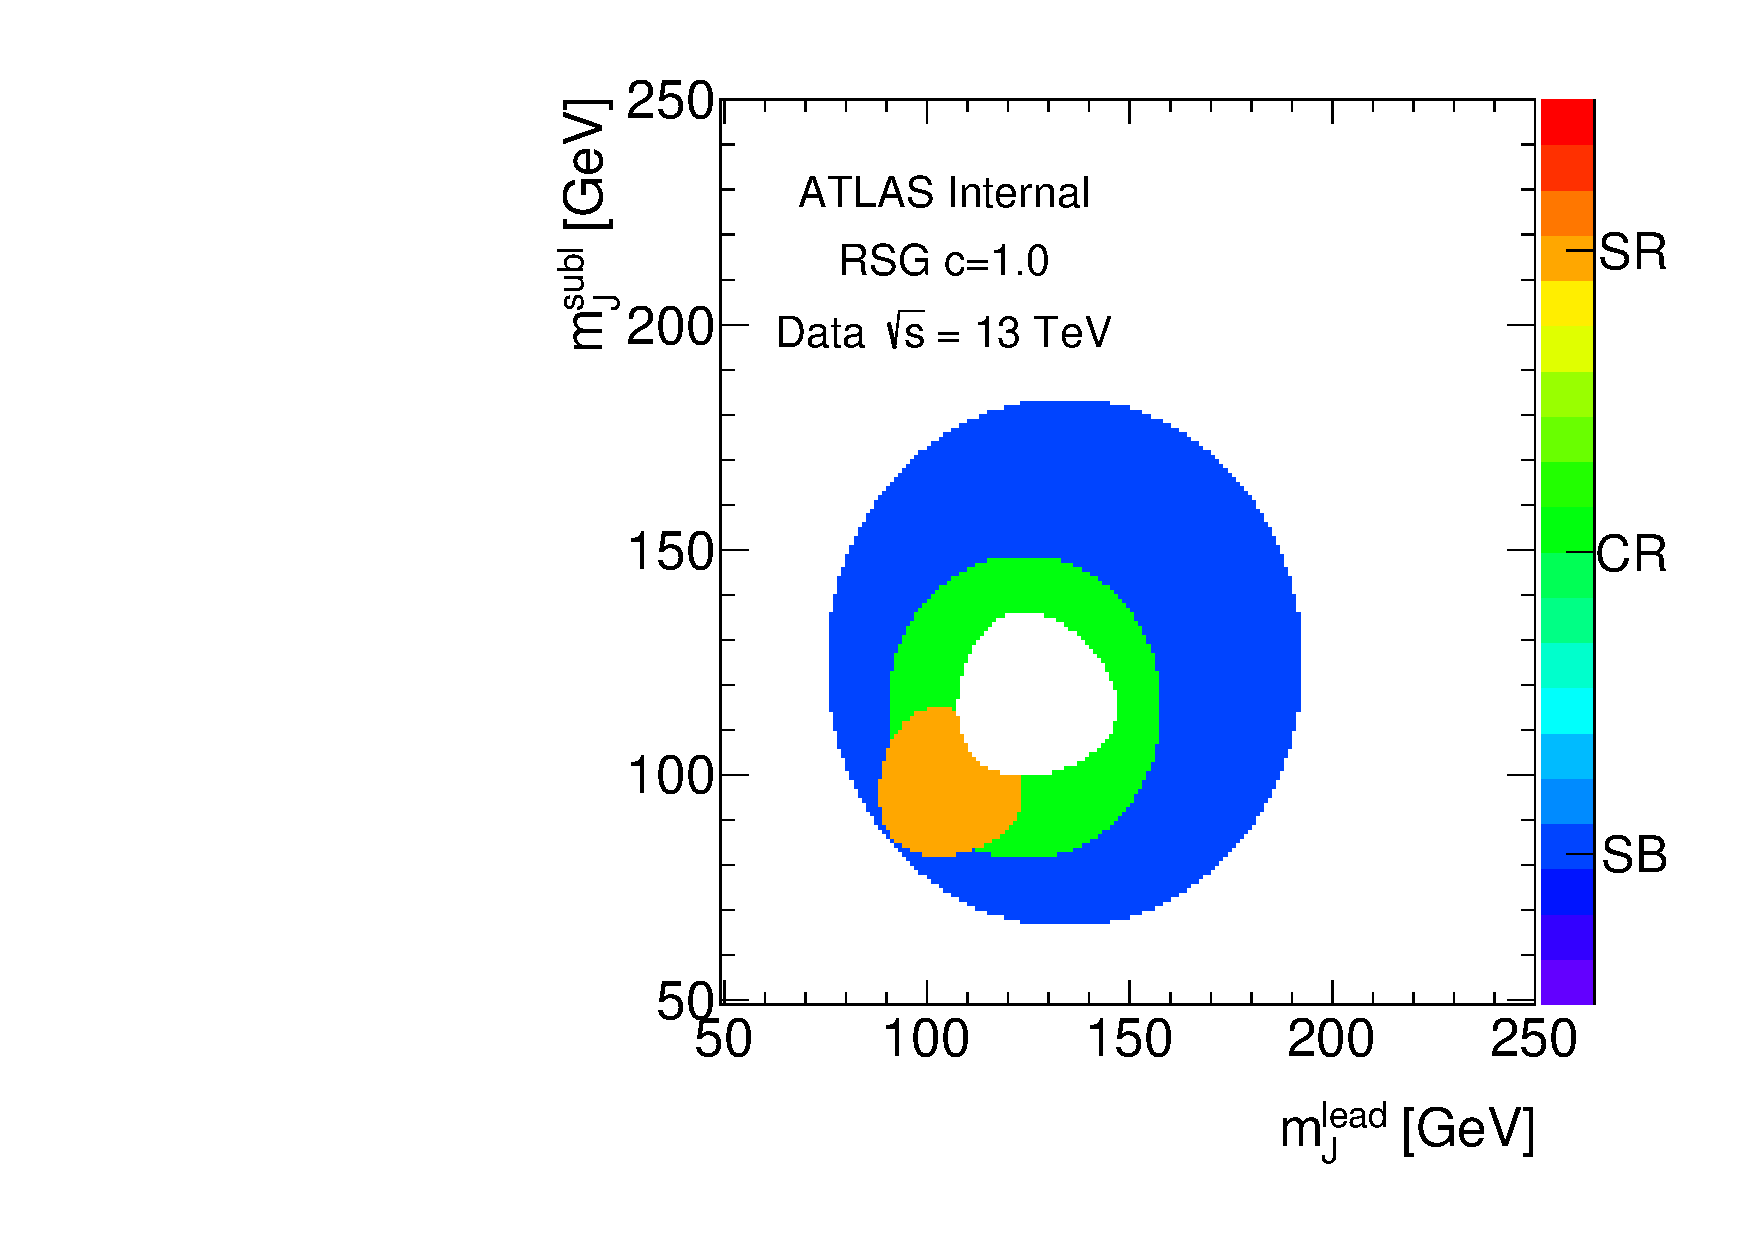
\includegraphics[width=0.4\textwidth,angle=-90]{figures/boosted/ZZ/Compare_NoTag_mH0H1.pdf}
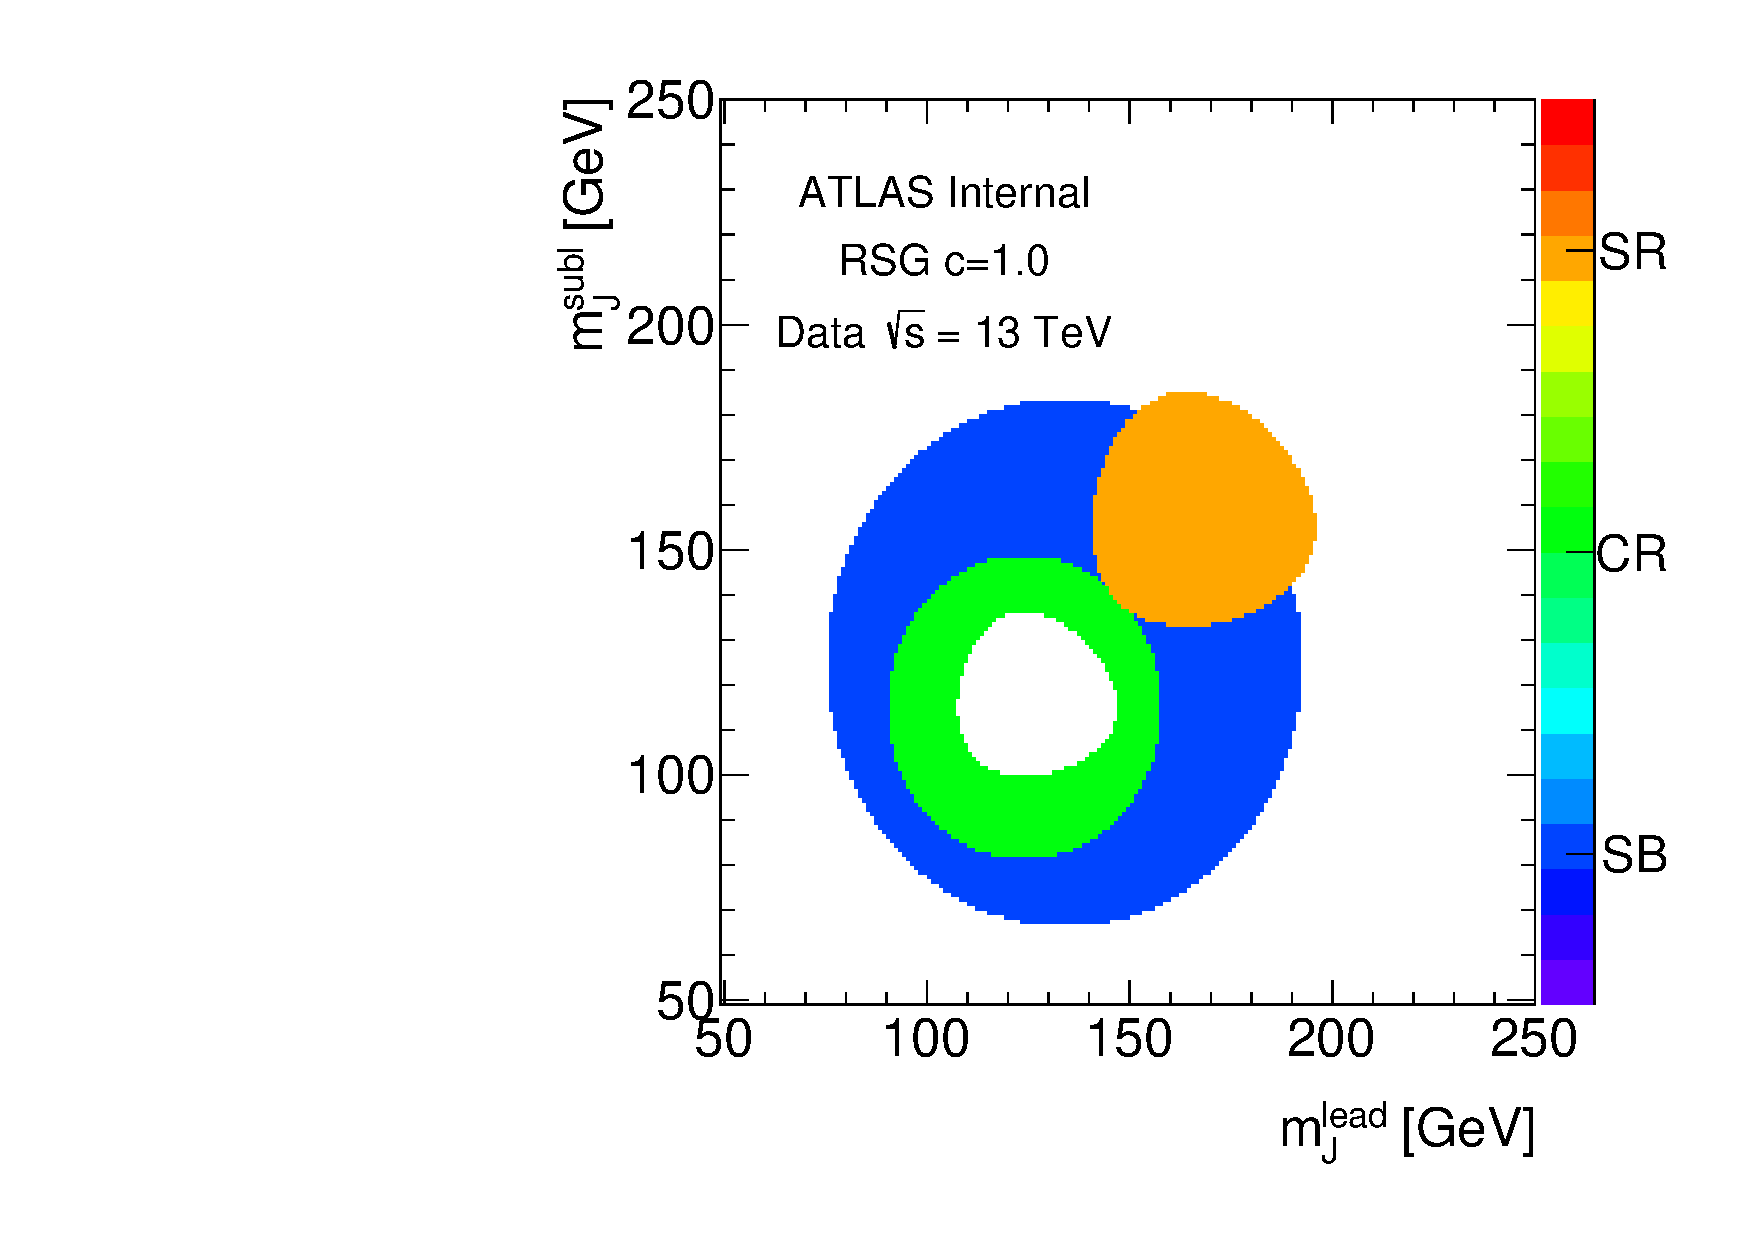
\includegraphics[width=0.4\textwidth,angle=-90]{figures/boosted/TT/Compare_NoTag_mH0H1.pdf}
\end{center}
\caption{Illustration of ZZ (left) and TT (right) signal region as shown in the orange shaded region. Control region shown in green, and Sideband region in blue. The white circle in the midde is the real Signal region, and it is blinded.}
\label{CRSB:ZZIllustration}
\end{figure}

%%\paragraph{}
The summary of background estimation for ZZ signal region can be found in Table \ref{CRSB:SummaryTable_ZZ_4b}, ~\ref{CRSB:SummaryTable_ZZ_3b} and ~\ref{CRSB:SummaryTable_ZZ_2b}. The difference between data and prediction in ZZ signal region is summarized in Table \ref{CRSB:DataPred_ZZSR} for all the regions. The discrepancy between data and prediction is either covered by statistical uncertainty of data or comparable with data statistical uncertainty in $4b$, $3b$ and $2bs$ ZZ SR respectively. We further check the kinematic distribution between data and prediction in ZZ SR, as shown in Figure \ref{CRSB:ZZSR_Distribution}. The data agrees with prediction well in general, though a few bins might not agree perfectly. The difference from $4b$ CR region test is 17$\%$, which is smaller than the $4b$ ZZ region difference. But the statistical uncertainty in ZZ region (yield 37) is much higher compared with our CR regions (min yield 76), hence the CR region with more statistical power is still used for the non-closure uncertainty.

%%\paragraph{}
The summary of background estimation for TT signal region can be found in Table \ref{CRSB:SummaryTable_TT_4b}, ~\ref{CRSB:SummaryTable_TT_3b} and ~\ref{CRSB:SummaryTable_TT_2b}. The difference between data and prediction in TT signal region is summarized in Table \ref{CRSB:DataPred_TTSR} for all the regions. The discrepancy between data and prediction is either covered by statistical uncertainty of data or comparable with data statistical uncertainty in $4b$, $3b$ and $2bs$ TT SR respectively. We further check the kinematic distribution between data and prediction in TT SR, as shown in Figure \ref{CRSB:TTSR_Distribution}. The data agrees with prediction well in general, though a few bins might not agree perfectly. 

%%\paragraph{}
Based on all the variation tests done above, we think there is no need to introduce extra uncertainty on non-closure systematics since most of the data/prediction disagreements are well covered by the data statistical uncertainty.

\begin{table}[htbp!]
\begin{center}
\begin{footnotesize} 
\begin{tabular}{c|c|c|c} 
FourTag & Sideband & Control & Signal \\ 
\hline\hline 
QCD Est & 166.65 $\pm$ 2.88 & 45.83 $\pm$ 1.51 & 27.37 $\pm$ 1.16\\ 
$t\bar{t}$ Est.  & 27.52 $\pm$ 0.25 & 6.31 $\pm$ 0.14 & 0 $\pm$ 0\\ 
$Z+jets$ & 0 $\pm$ 0 & 6.18 $\pm$ 5.12 & 0 $\pm$ 0\\ 
Total Bkg Est & 194.17 $\pm$ 2.89 & 58.32 $\pm$ 5.34 & 27.37 $\pm$ 1.16\\ 
Data & 194.0 $\pm$ 13.93 & 54.0 $\pm$ 7.35 & 37.0 $\pm$ 6.08\\ 
$c=1.0$,$m=1.0TeV$ & 2.45 $\pm$ 0.098 & 4.47 $\pm$ 0.13 & 0.99 $\pm$ 0.063\\ 
$c=1.0$,$m=2.0TeV$ & 0.032 $\pm$ 0.0015 & 0.075 $\pm$ 0.0022 & 0.028 $\pm$ 0.0014\\ 
$c=1.0$,$m=3.0TeV$ & 0.00029 $\pm$ 3.5e-05 & 0.00064 $\pm$ 5e-05 & 0.0002 $\pm$ 2.7e-05\\ 
\hline\hline 
\end{tabular} 
\end{footnotesize} 
\newline 

\end{center}
\caption{Background prediction in SR/CR/SB for ZZ SR in $4b$-tag region. Uncertainties are stat only.}
\label{CRSB:SummaryTable_ZZ_4b}
\end{table}

\begin{table}[htbp!]
\begin{center}
\begin{footnotesize} 
\begin{tabular}{c|c|c|c} 
ThreeTag & Sideband & Control & Signal \\ 
\hline\hline 
& & & \\ 
QCD Est & 3344.46 $\pm$ 26.85 & 998.41 $\pm$ 14.63 & 637.78 $\pm$ 11.87\\ 
$t\bar{t}$ Est.  & 826.66 $\pm$ 25.11 & 136.58 $\pm$ 10.23 & 30.07 $\pm$ 1.24\\ 
$Z+jets$ & 32.49 $\pm$ 11.34 & 8.22 $\pm$ 5.29 & 3.3 $\pm$ 2.0\\ 
Total Bkg Est & 4203.61 $\pm$ 38.47 & 1143.2 $\pm$ 18.62 & 671.15 $\pm$ 12.11\\ 
Data & 4203.0 $\pm$ 64.83 & 1108.0 $\pm$ 33.29 & 645.0 $\pm$ 25.4\\ 
$c=1.0$,$m=1.0TeV$ & 7.56 $\pm$ 0.18 & 9.84 $\pm$ 0.2 & 3.05 $\pm$ 0.11\\ 
$c=1.0$,$m=2.0TeV$ & 0.15 $\pm$ 0.0033 & 0.27 $\pm$ 0.0046 & 0.12 $\pm$ 0.003\\ 
$c=1.0$,$m=3.0TeV$ & 0.0034 $\pm$ 0.00012 & 0.0056 $\pm$ 0.00016 & 0.0021 $\pm$ 9.5e-05\\ 
& & & \\ 
\hline\hline 
\end{tabular} 
\end{footnotesize} 
\newline 

\end{center}
\caption{Background prediction in SR/CR/SB for ZZ SR in $3b$-tag region. Uncertainties are stat only.}
\label{CRSB:SummaryTable_ZZ_3b}
\end{table}

\begin{table}[htbp!]
\begin{center}
\begin{footnotesize} 
\begin{tabular}{c|c|c|c} 
TwoTag split & Sideband & Control & Signal \\ 
\hline\hline 
QCD Est & 16387.44 $\pm$ 37.6 & 4827.76 $\pm$ 19.86 & 3026.83 $\pm$ 15.61\\ 
$t\bar{t}$ Est.  & 7671.95 $\pm$ 69.14 & 1229.96 $\pm$ 26.54 & 332.29 $\pm$ 13.66\\ 
$Z+jets$ & 44.37 $\pm$ 13.23 & 13.34 $\pm$ 6.6 & 36.47 $\pm$ 12.88\\ 
Total Bkg Est & 24103.77 $\pm$ 79.8 & 6071.07 $\pm$ 33.8 & 3395.59 $\pm$ 24.42\\ 
Data & 24104.0 $\pm$ 155.25 & 6261.0 $\pm$ 79.13 & 3258.0 $\pm$ 57.08\\ 
$c=1.0$,$m=1.0TeV$ & 4.57 $\pm$ 0.14 & 4.65 $\pm$ 0.14 & 1.91 $\pm$ 0.089\\ 
$c=1.0$,$m=2.0TeV$ & 0.16 $\pm$ 0.0038 & 0.26 $\pm$ 0.0047 & 0.12 $\pm$ 0.0032\\ 
$c=1.0$,$m=3.0TeV$ & 0.012 $\pm$ 0.00024 & 0.019 $\pm$ 0.00029 & 0.0085 $\pm$ 0.00019\\ 
\hline\hline 
\end{tabular} 
\end{footnotesize} 
\newline 

\end{center}
\caption{Background prediction in SR/CR/SB for ZZ SR in $2bs$-tag region. Uncertainties are stat only.}
\label{CRSB:SummaryTable_ZZ_2b}
\end{table}

\begin{table}[htbp!]
\begin{center}
\begin{footnotesize} 
\begin{tabular}{c|c|c|c} 
ZZ Signal Region & Data & Prediction & (Predict - Data)/Data \\ 
\hline\hline 
FourTag & 37.0 $\pm$ 6.08 & 27.37 $\pm$ 1.16 & -26.0 $\%$  $\pm$ 15.3 $\%$ \\ 
\hline 
ThreeTag & 645.0 $\pm$ 25.4 & 671.15 $\pm$ 12.11 & 4.05 $\%$  $\pm$ 5.97 $\%$ \\ 
\hline 
TwoTag split & 3258.0 $\pm$ 57.08 & 3395.59 $\pm$ 24.42 & 4.22 $\%$  $\pm$ 2.58 $\%$ \\ 
\hline\hline 
\end{tabular} 
\end{footnotesize} 
\newline 

\end{center}
\caption{Agreement between data and prediction in ZZ SR in $4b$, $3b$ and $2bs$ regions.}
\label{CRSB:DataPred_ZZSR}
\end{table}

\begin{figure}[htbp!]
\begin{center}
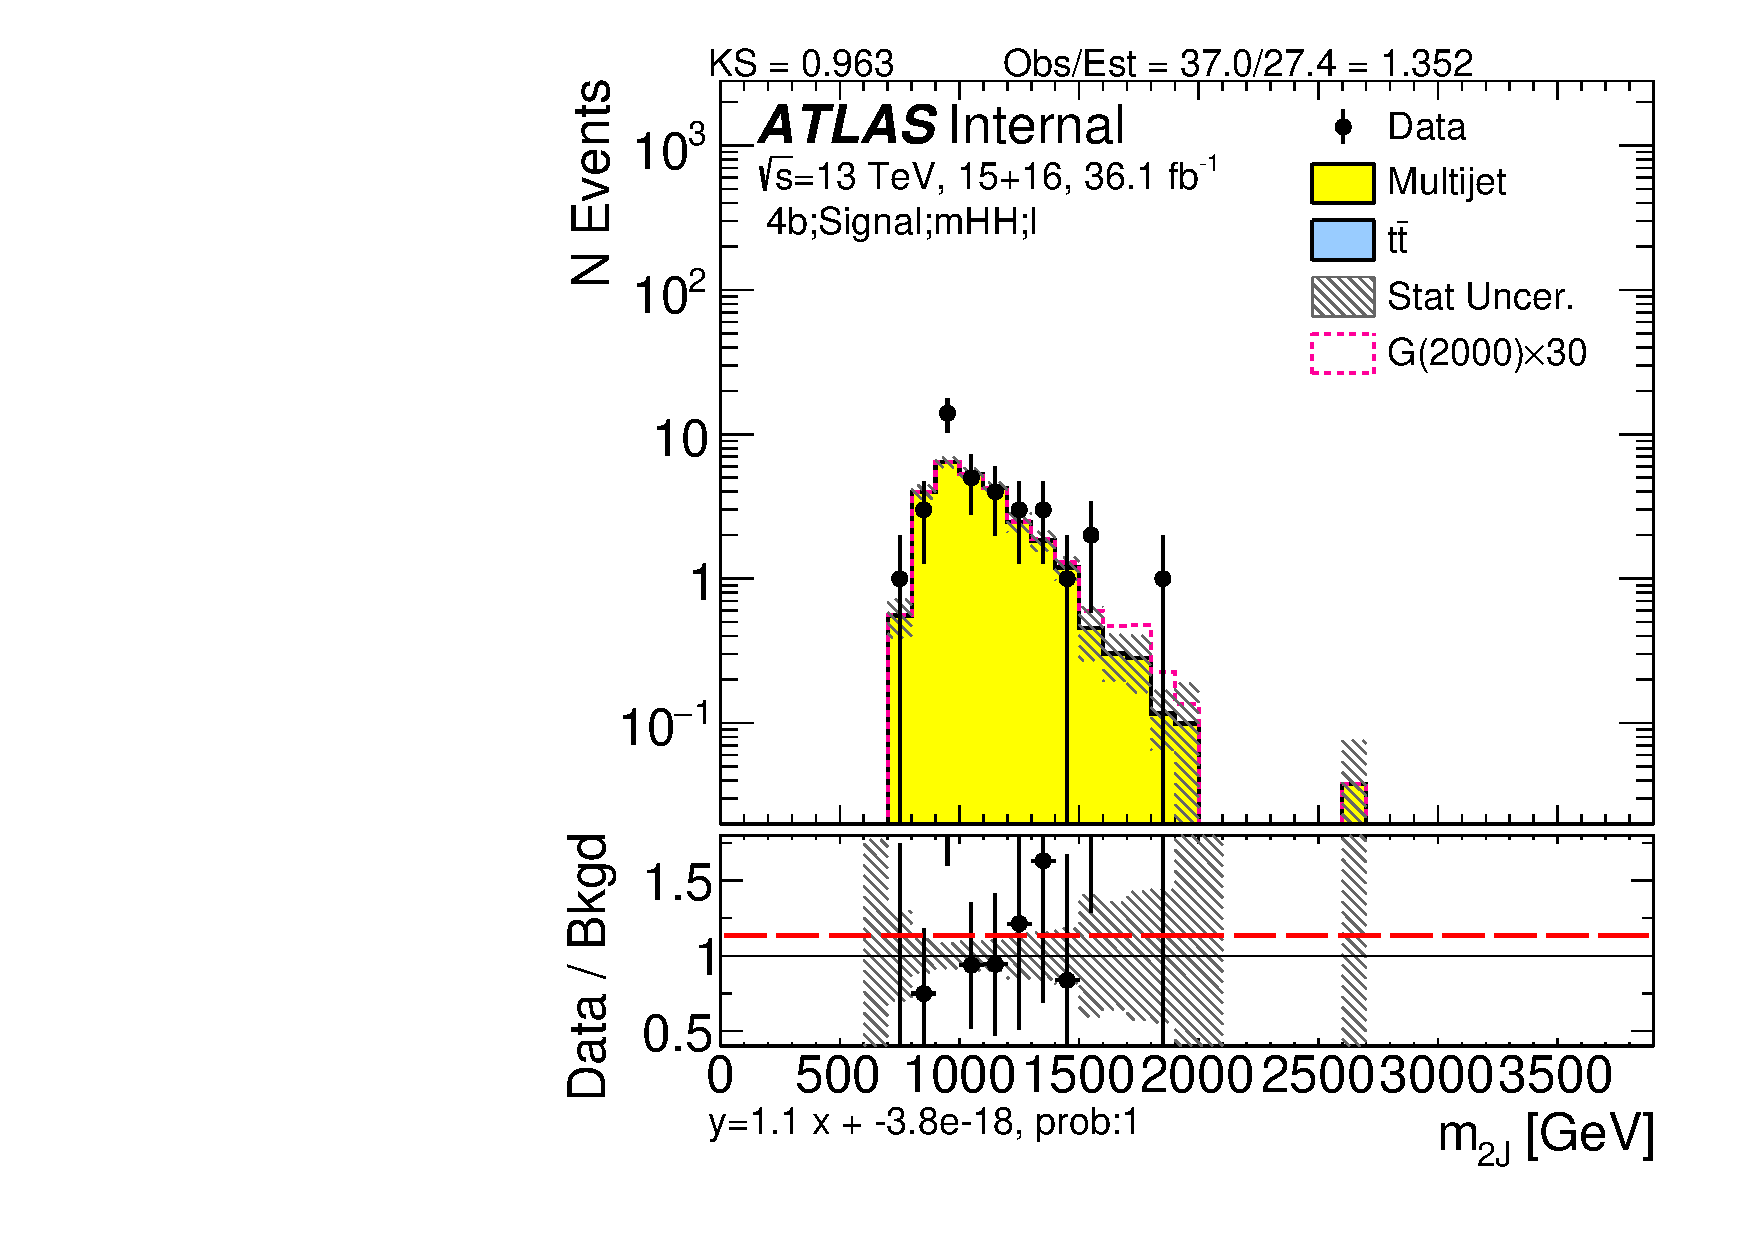
\includegraphics[width=0.45\textwidth,angle=-90]{figures/boosted/ZZ/Moriond_ZZ_FourTag_Signal_mHH_l_1.pdf}
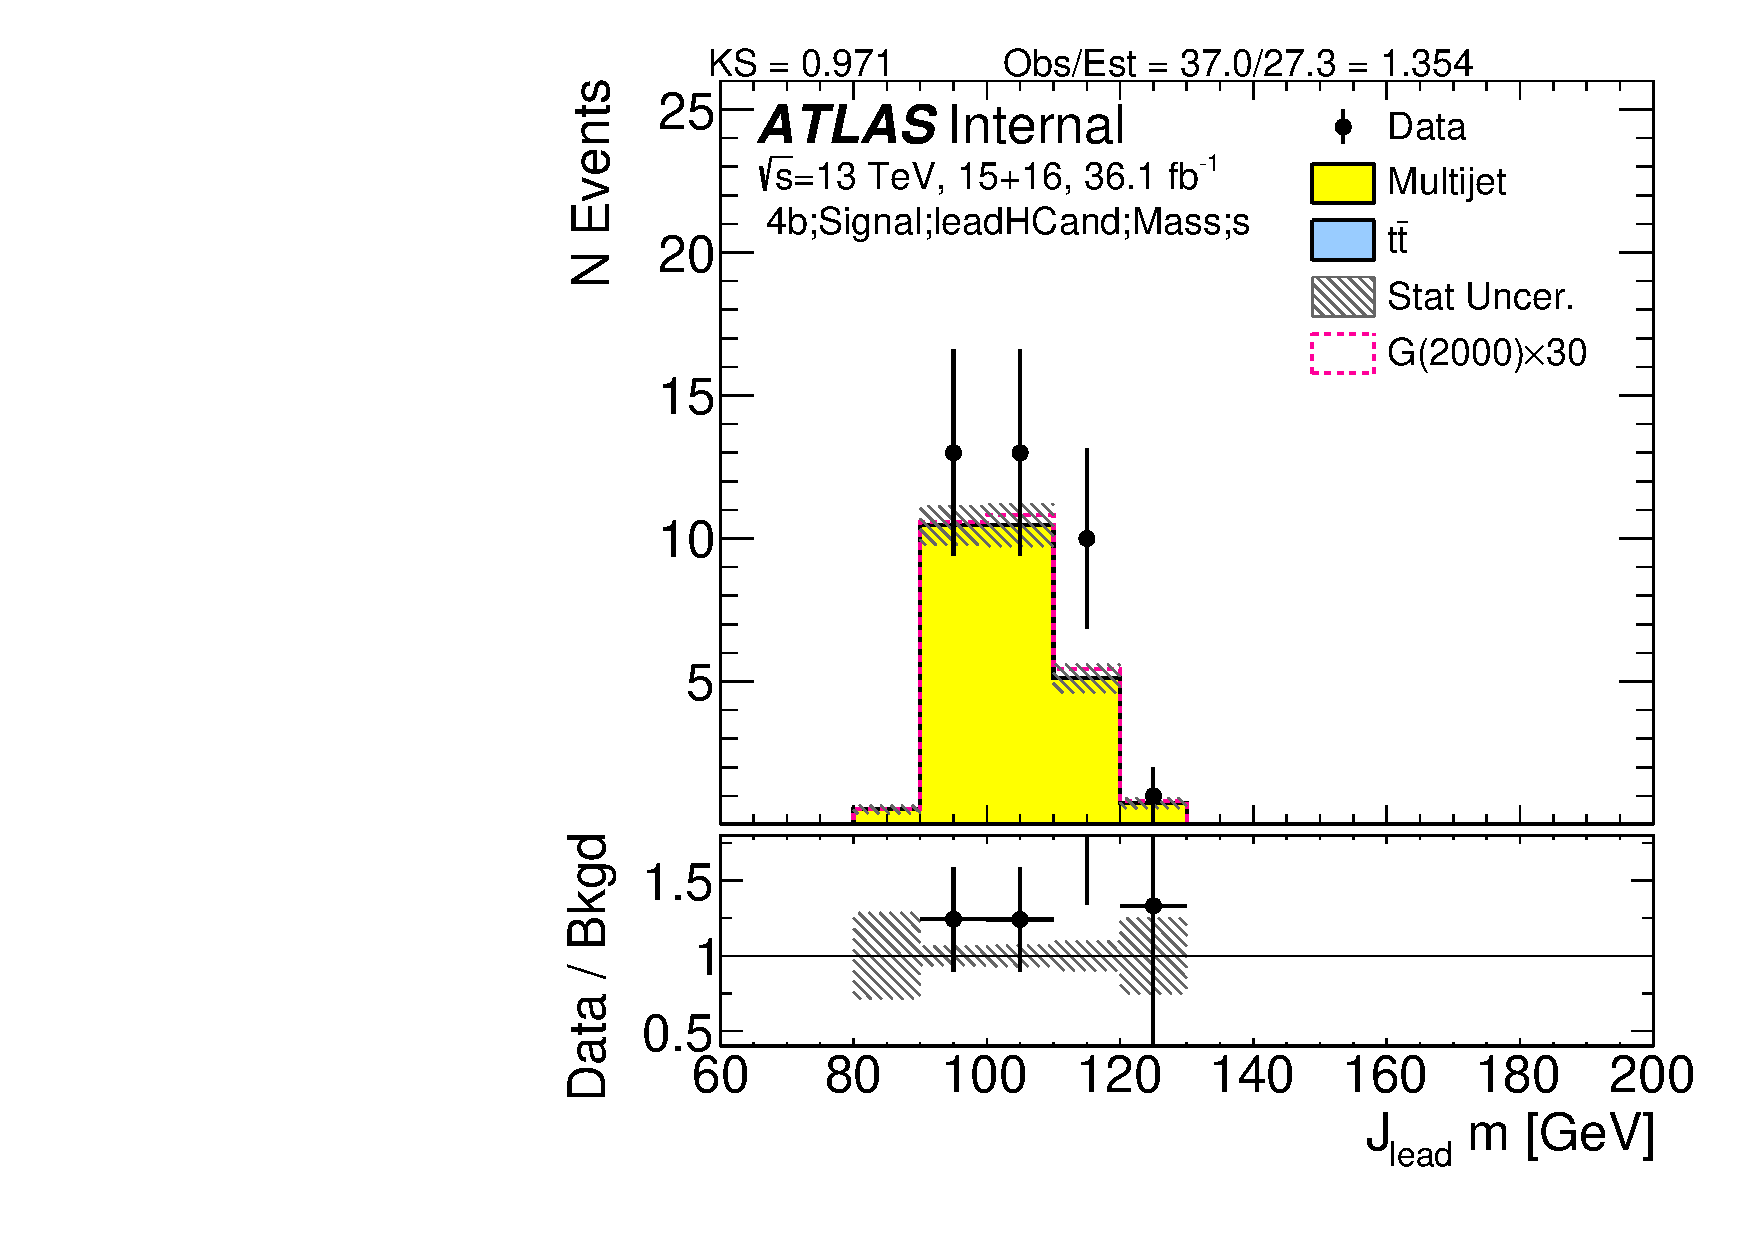
\includegraphics[width=0.45\textwidth,angle=-90]{figures/boosted/ZZ/Moriond_ZZ_FourTag_Signal_leadHCand_Mass_s.pdf}\\
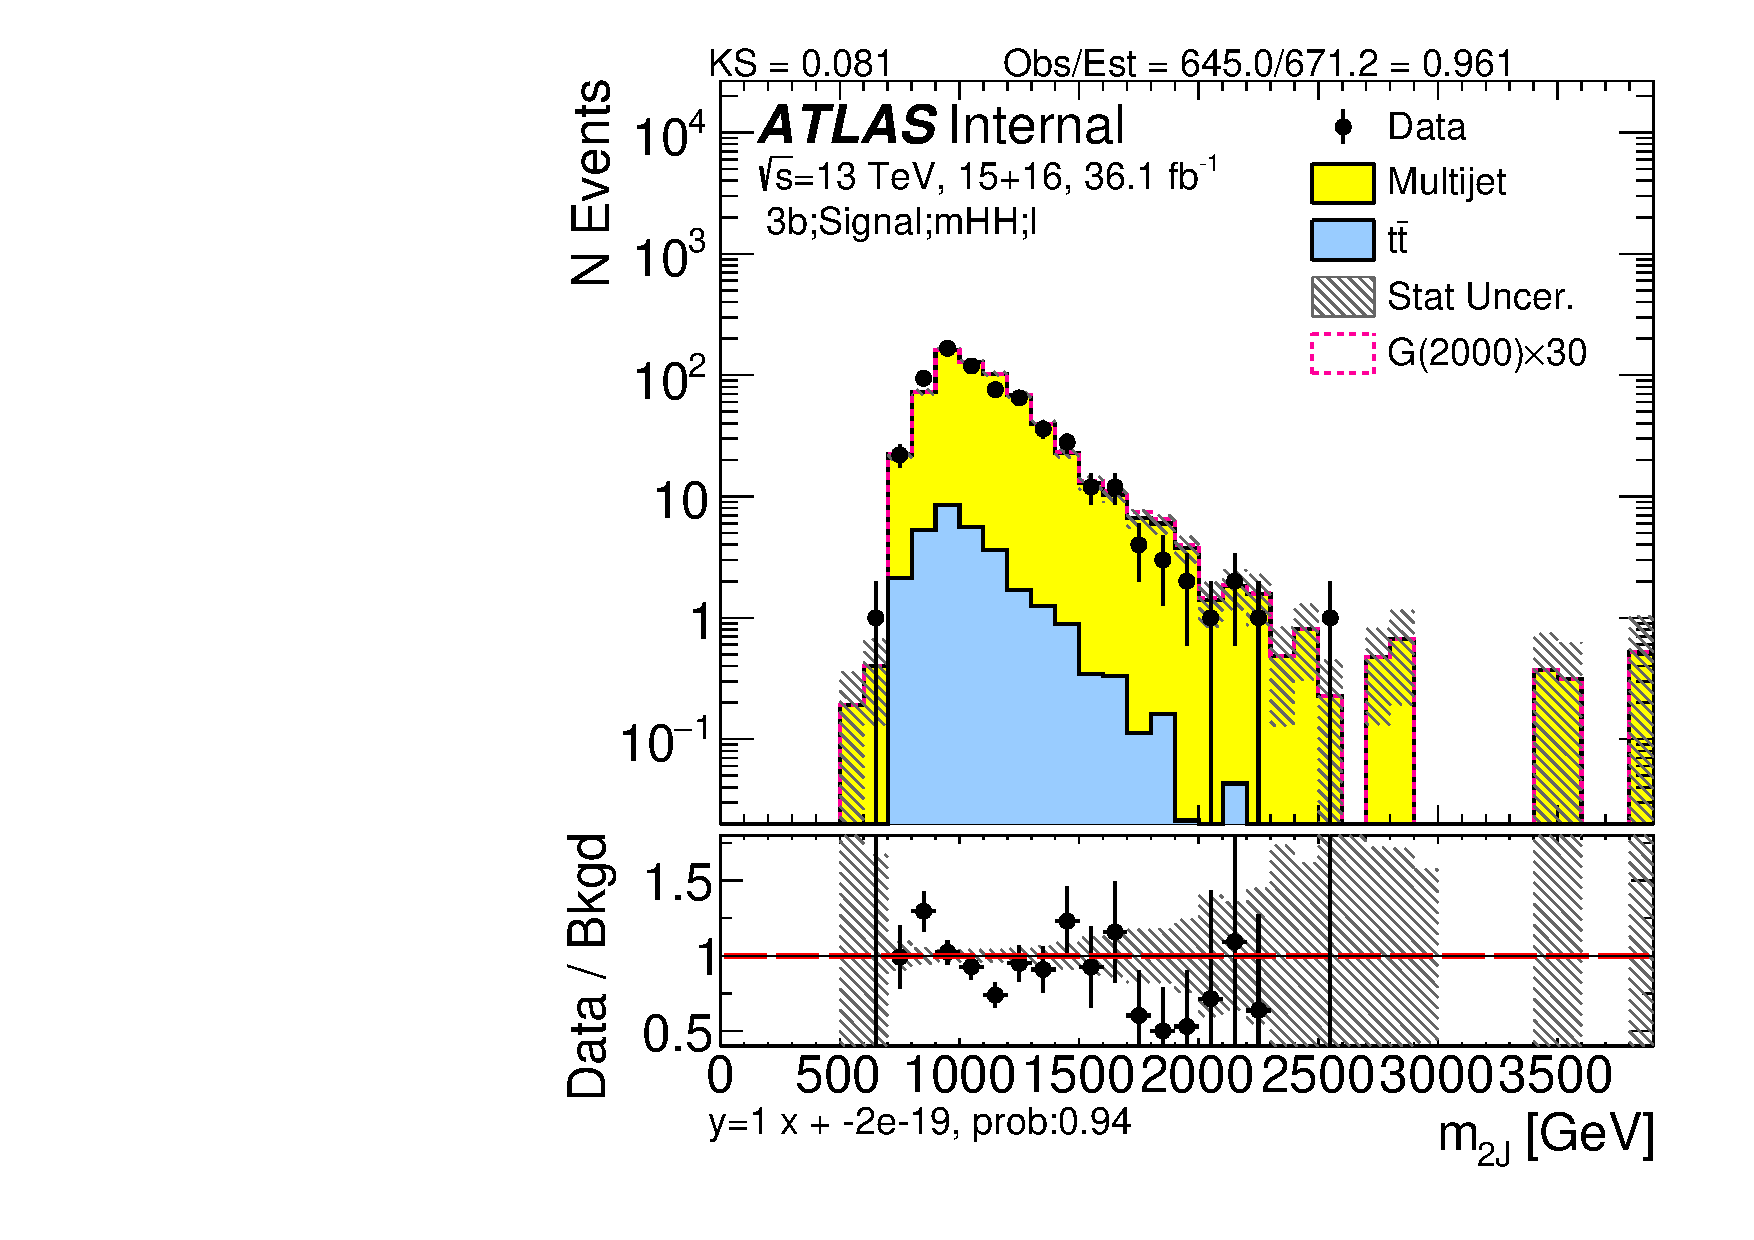
\includegraphics[width=0.45\textwidth,angle=-90]{figures/boosted/ZZ/Moriond_ZZ_ThreeTag_Signal_mHH_l_1.pdf}
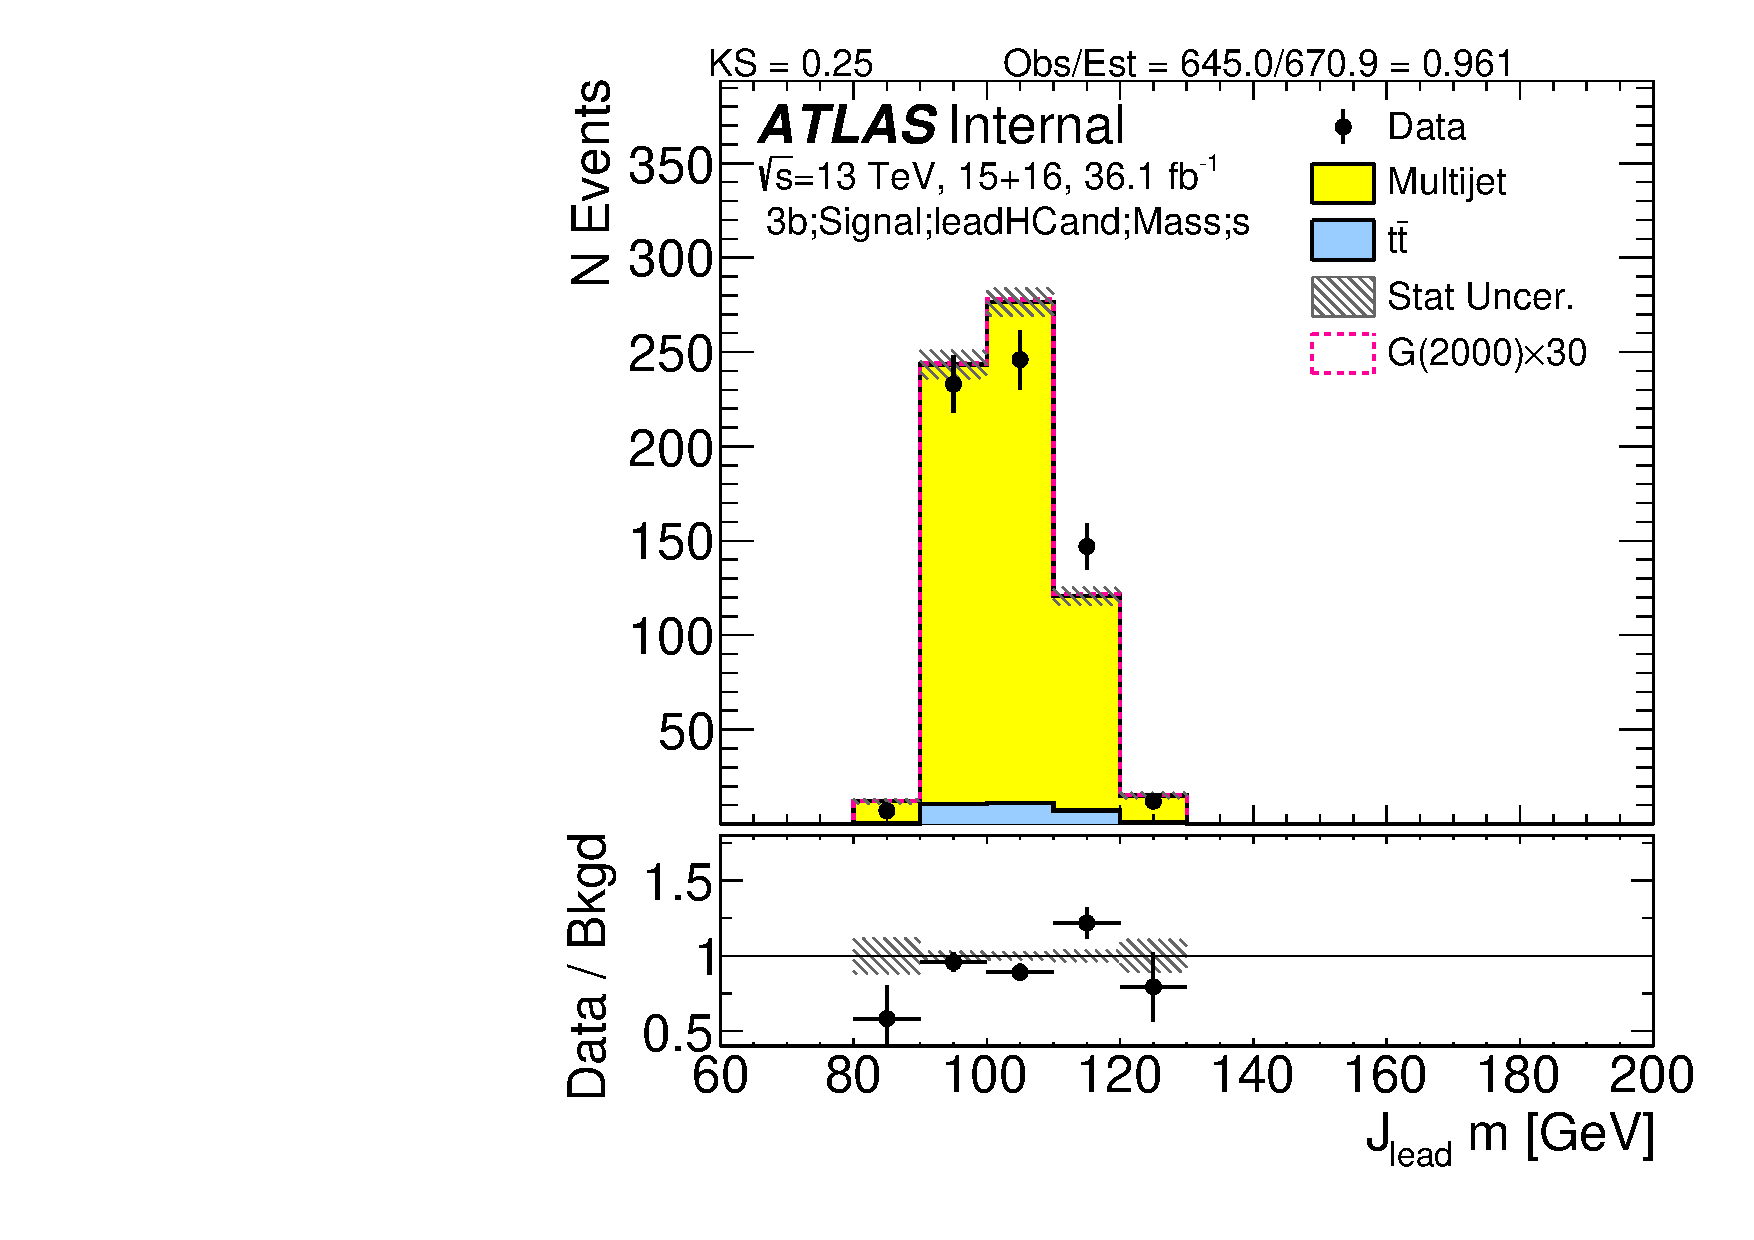
\includegraphics[width=0.45\textwidth,angle=-90]{figures/boosted/ZZ/Moriond_ZZ_ThreeTag_Signal_leadHCand_Mass_s.pdf}\\
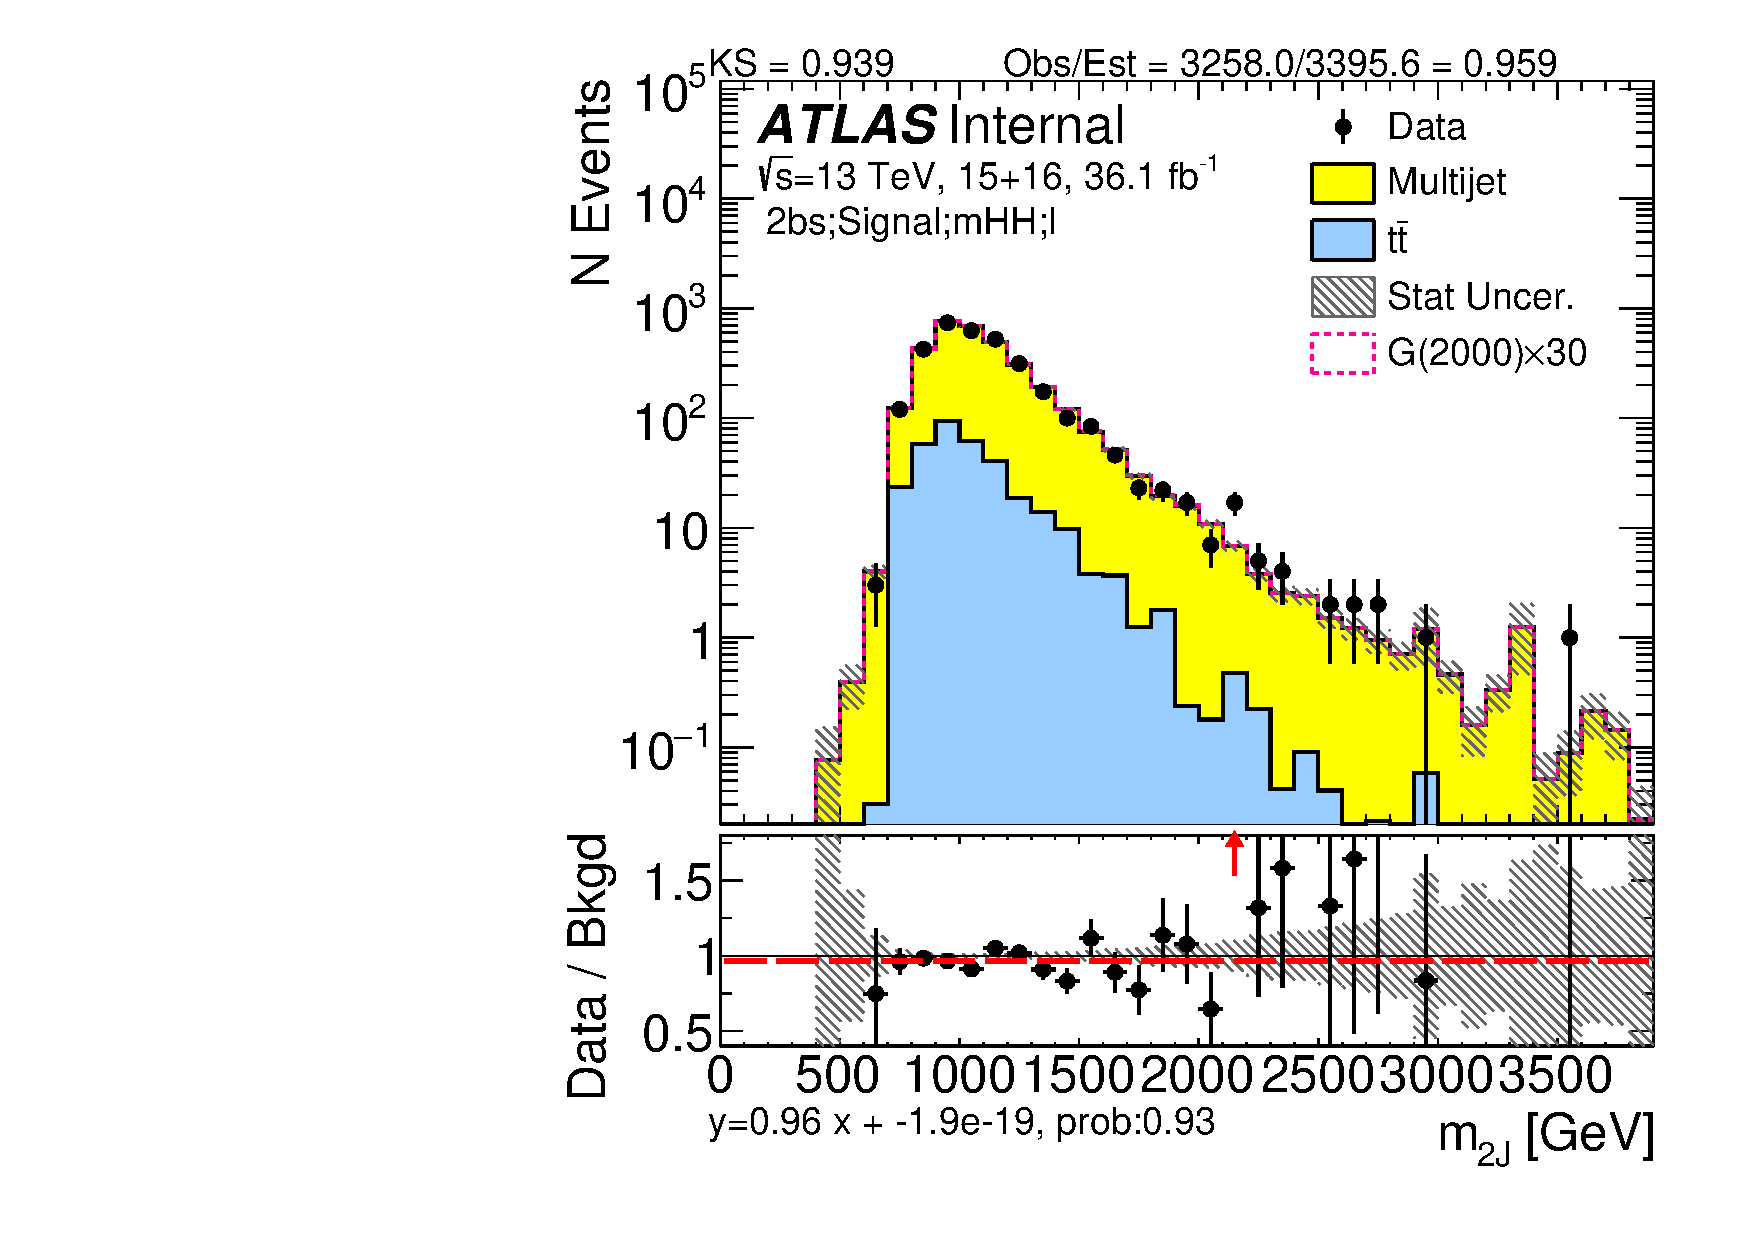
\includegraphics[width=0.45\textwidth,angle=-90]{figures/boosted/ZZ/Moriond_ZZ_TwoTag_split_Signal_mHH_l_1.pdf}
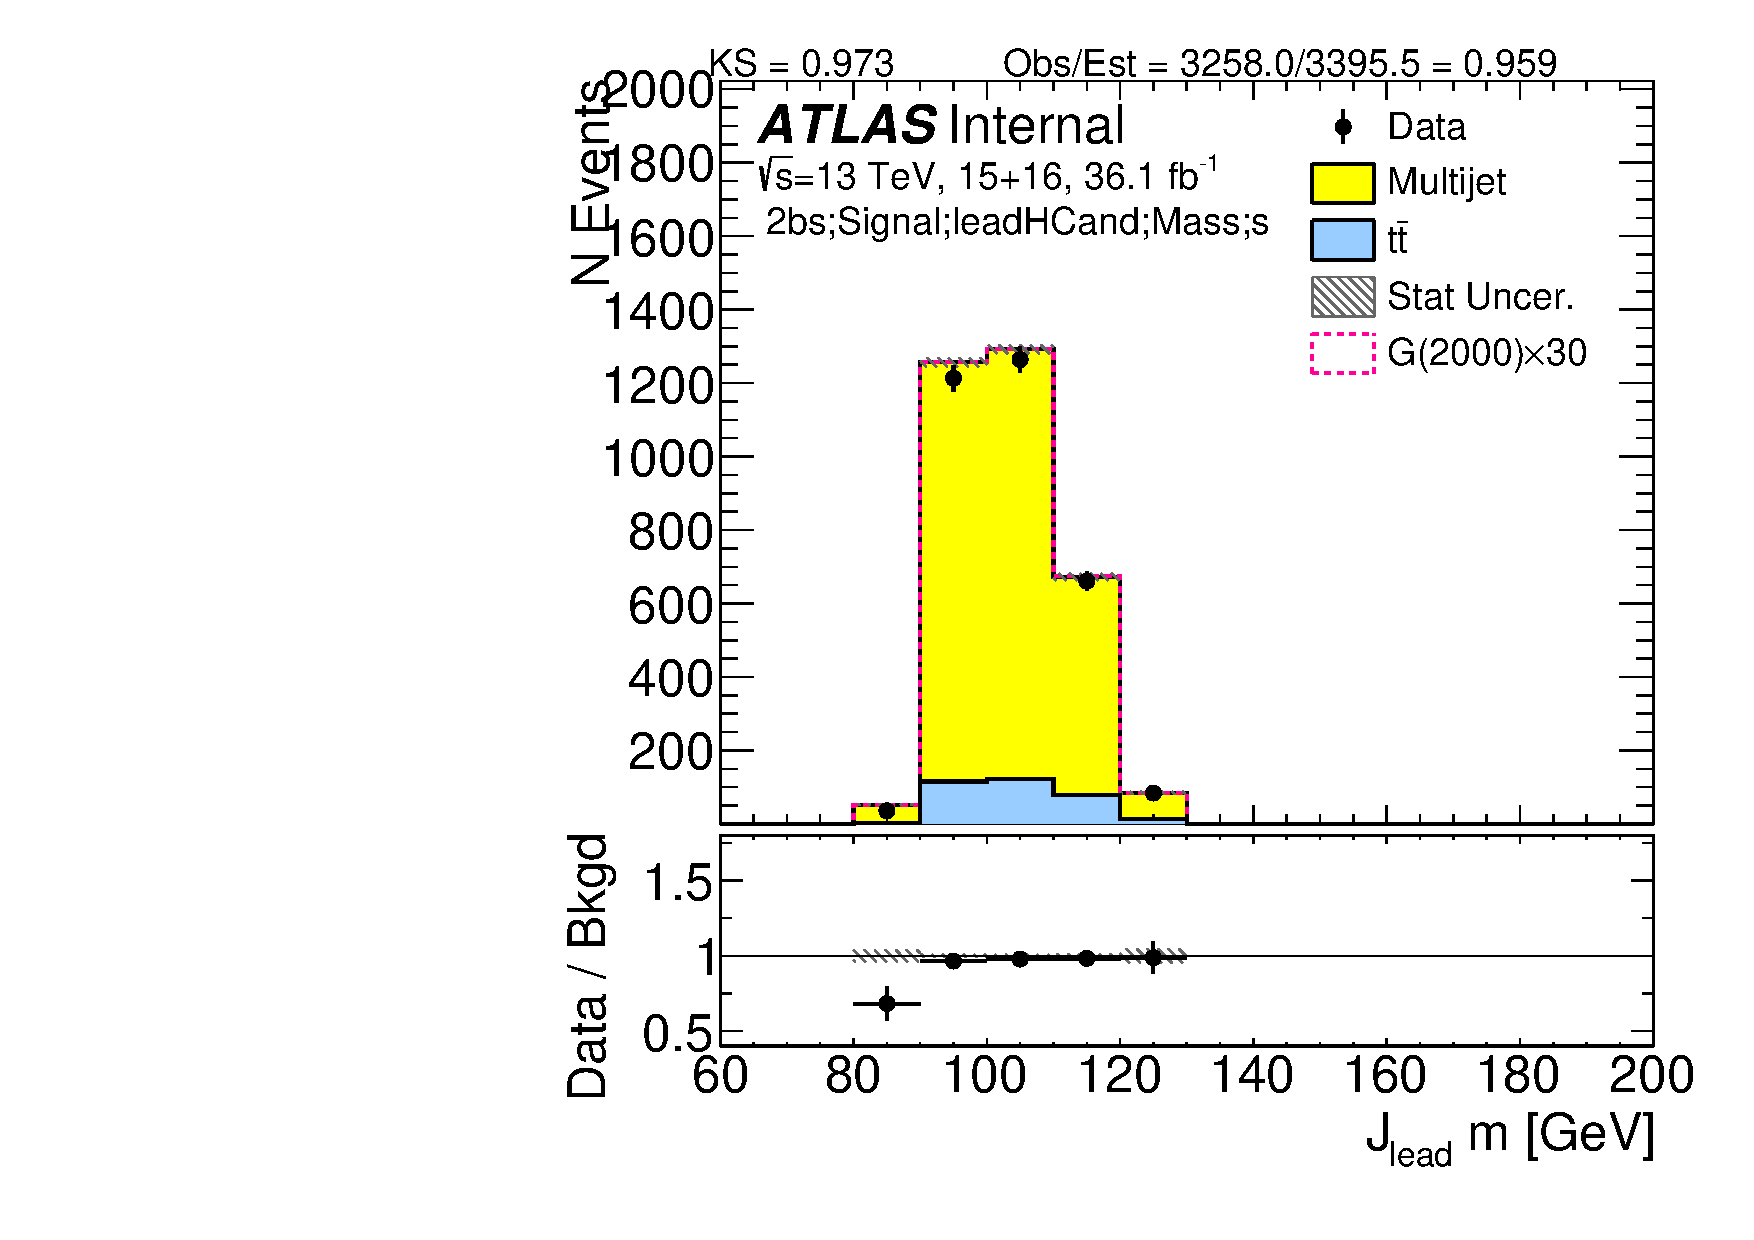
\includegraphics[width=0.45\textwidth,angle=-90]{figures/boosted/ZZ/Moriond_ZZ_TwoTag_split_Signal_leadHCand_Mass_s.pdf}\\
\end{center}
\caption{ZZ signal region distribution of di-jet mass (left column) and leading large-R jet mass (right column) in low mass signal, for $4b$ (top row), $3b$(middle row) and $2b$ split (bottom row). The plots are with only statistical uncertainty.}
\label{CRSB:ZZSR_Distribution}
\end{figure}

\begin{table}[htbp!]
\begin{center}
\begin{footnotesize} 
\begin{tabular}{c|c|c|c} 
FourTag & Sideband & Control & Signal \\ 
\hline\hline 
& & & \\ 
QCD Est & 152.28 $\pm$ 2.72 & 63.47 $\pm$ 1.77 & 28.6 $\pm$ 1.21\\ 
$t\bar{t}$ Est.  & 19.86 $\pm$ 0.22 & 7.45 $\pm$ 0.15 & 15.02 $\pm$ 0.2\\ 
$Z+jets$ & 0 $\pm$ 0 & 6.18 $\pm$ 5.12 & 0 $\pm$ 0\\ 
Total Bkg Est & 172.14 $\pm$ 2.73 & 77.1 $\pm$ 5.42 & 43.62 $\pm$ 1.23\\ 
Data & 172.0 $\pm$ 13.11 & 81.0 $\pm$ 9.0 & 46.0 $\pm$ 6.78\\ 
$c=1.0$,$m=1.0TeV$ & 2.38 $\pm$ 0.097 & 5.4 $\pm$ 0.15 & 0.15 $\pm$ 0.024\\ 
$c=1.0$,$m=2.0TeV$ & 0.033 $\pm$ 0.0015 & 0.1 $\pm$ 0.0026 & 0.0011 $\pm$ 0.00027\\ 
$c=1.0$,$m=3.0TeV$ & 0.00031 $\pm$ 3.6e-05 & 0.0008 $\pm$ 5.6e-05 & 1.5e-05 $\pm$ 7.7e-06\\ 
& & & \\ 
\hline\hline 
\end{tabular} 
\end{footnotesize} 
\newline 

\end{center}
\caption{Background prediction in SR/CR/SB for TT SR in $4b$-tag region. Uncertainties are stat only.}
\label{CRSB:SummaryTable_TT_4b}
\end{table}

\begin{table}[htbp!]
\begin{center}
\begin{footnotesize} 
\begin{tabular}{c|c|c|c} 
ThreeTag & Sideband & Control & Signal \\ 
\hline\hline 
QCD Est & 3106.11 $\pm$ 25.79 & 1427.41 $\pm$ 17.53 & 570.01 $\pm$ 11.6\\ 
$t\bar{t}$ Est.  & 495.21 $\pm$ 18.75 & 148.55 $\pm$ 10.21 & 406.57 $\pm$ 5.42\\ 
$Z+jets$ & 32.5 $\pm$ 11.34 & 11.21 $\pm$ 5.65 & 0.3 $\pm$ 0.3\\ 
Total Bkg Est & 3633.82 $\pm$ 33.85 & 1587.17 $\pm$ 21.05 & 976.88 $\pm$ 12.81\\ 
Data & 3633.0 $\pm$ 60.27 & 1553.0 $\pm$ 39.41 & 1017.0 $\pm$ 31.89\\ 
$c=1.0$,$m=1.0TeV$ & 7.57 $\pm$ 0.18 & 12.58 $\pm$ 0.23 & 0.32 $\pm$ 0.037\\ 
$c=1.0$,$m=2.0TeV$ & 0.15 $\pm$ 0.0034 & 0.38 $\pm$ 0.0054 & 0.0047 $\pm$ 0.0006\\ 
$c=1.0$,$m=3.0TeV$ & 0.0034 $\pm$ 0.00012 & 0.0075 $\pm$ 0.00018 & 0.00023 $\pm$ 3.3e-05\\ 
\hline\hline 
\end{tabular} 
\end{footnotesize} 
\newline 

\end{center}
\caption{Background prediction in SR/CR/SB for TT SR in $3b$-tag region. Uncertainties are stat only.}
\label{CRSB:SummaryTable_TT_3b}
\end{table}

\begin{table}[htbp!]
\begin{center}
\begin{footnotesize} 
\begin{tabular}{c|c|c|c} 
TwoTag split & Sideband & Control & Signal \\ 
\hline\hline 
QCD Est & 14980.05 $\pm$ 35.33 & 6803.06 $\pm$ 23.41 & 2817.92 $\pm$ 16.54\\ 
$t\bar{t}$ Est.  & 5170.92 $\pm$ 56.22 & 1468.85 $\pm$ 28.93 & 3628.91 $\pm$ 48.42\\ 
$Z+jets$ & 61.34 $\pm$ 16.04 & 26.44 $\pm$ 10.08 & 6.4 $\pm$ 5.05\\ 
Total Bkg Est & 20212.31 $\pm$ 68.31 & 8298.34 $\pm$ 38.56 & 6453.23 $\pm$ 51.41\\ 
Data & 20212.0 $\pm$ 142.17 & 8486.0 $\pm$ 92.12 & 6446.0 $\pm$ 80.29\\ 
$c=1.0$,$m=1.0TeV$ & 4.59 $\pm$ 0.14 & 6.33 $\pm$ 0.16 & 0.24 $\pm$ 0.033\\ 
$c=1.0$,$m=2.0TeV$ & 0.17 $\pm$ 0.0039 & 0.36 $\pm$ 0.0056 & 0.0066 $\pm$ 0.00077\\ 
$c=1.0$,$m=3.0TeV$ & 0.012 $\pm$ 0.00024 & 0.027 $\pm$ 0.00034 & 0.00089 $\pm$ 6.7e-05\\ 
\hline\hline 
\end{tabular} 
\end{footnotesize} 
\newline 

\end{center}
\caption{Background prediction in SR/CR/SB for TT SR in $2bs$-tag region. Uncertainties are stat only.}
\label{CRSB:SummaryTable_TT_2b}
\end{table}

\begin{table}[htbp!]
\begin{center}
\begin{footnotesize} 
\begin{tabular}{c|c|c|c} 
TT Signal Region & Data & Prediction & (Predict - Data)/Data \\ 
\hline\hline 
FourTag & 46.0 $\pm$ 6.78 & 43.62 $\pm$ 1.23 & -5.18 $\%$  $\pm$ 16.66 $\%$ \\ 
\hline 
ThreeTag & 1017.0 $\pm$ 31.89 & 976.88 $\pm$ 12.81 & -3.95 $\%$  $\pm$ 4.27 $\%$ \\ 
\hline 
TwoTag split & 6446.0 $\pm$ 80.29 & 6453.23 $\pm$ 51.41 & 0.11 $\%$  $\pm$ 2.04 $\%$ \\ 
\hline\hline 
\end{tabular} 
\end{footnotesize} 
\newline 

\end{center}
\caption{Agreement between data and prediction in TT SR in $4b$, $3b$ and $2bs$ regions.}
\label{CRSB:DataPred_TTSR}
\end{table}


\begin{figure}[htbp!]
\begin{center}
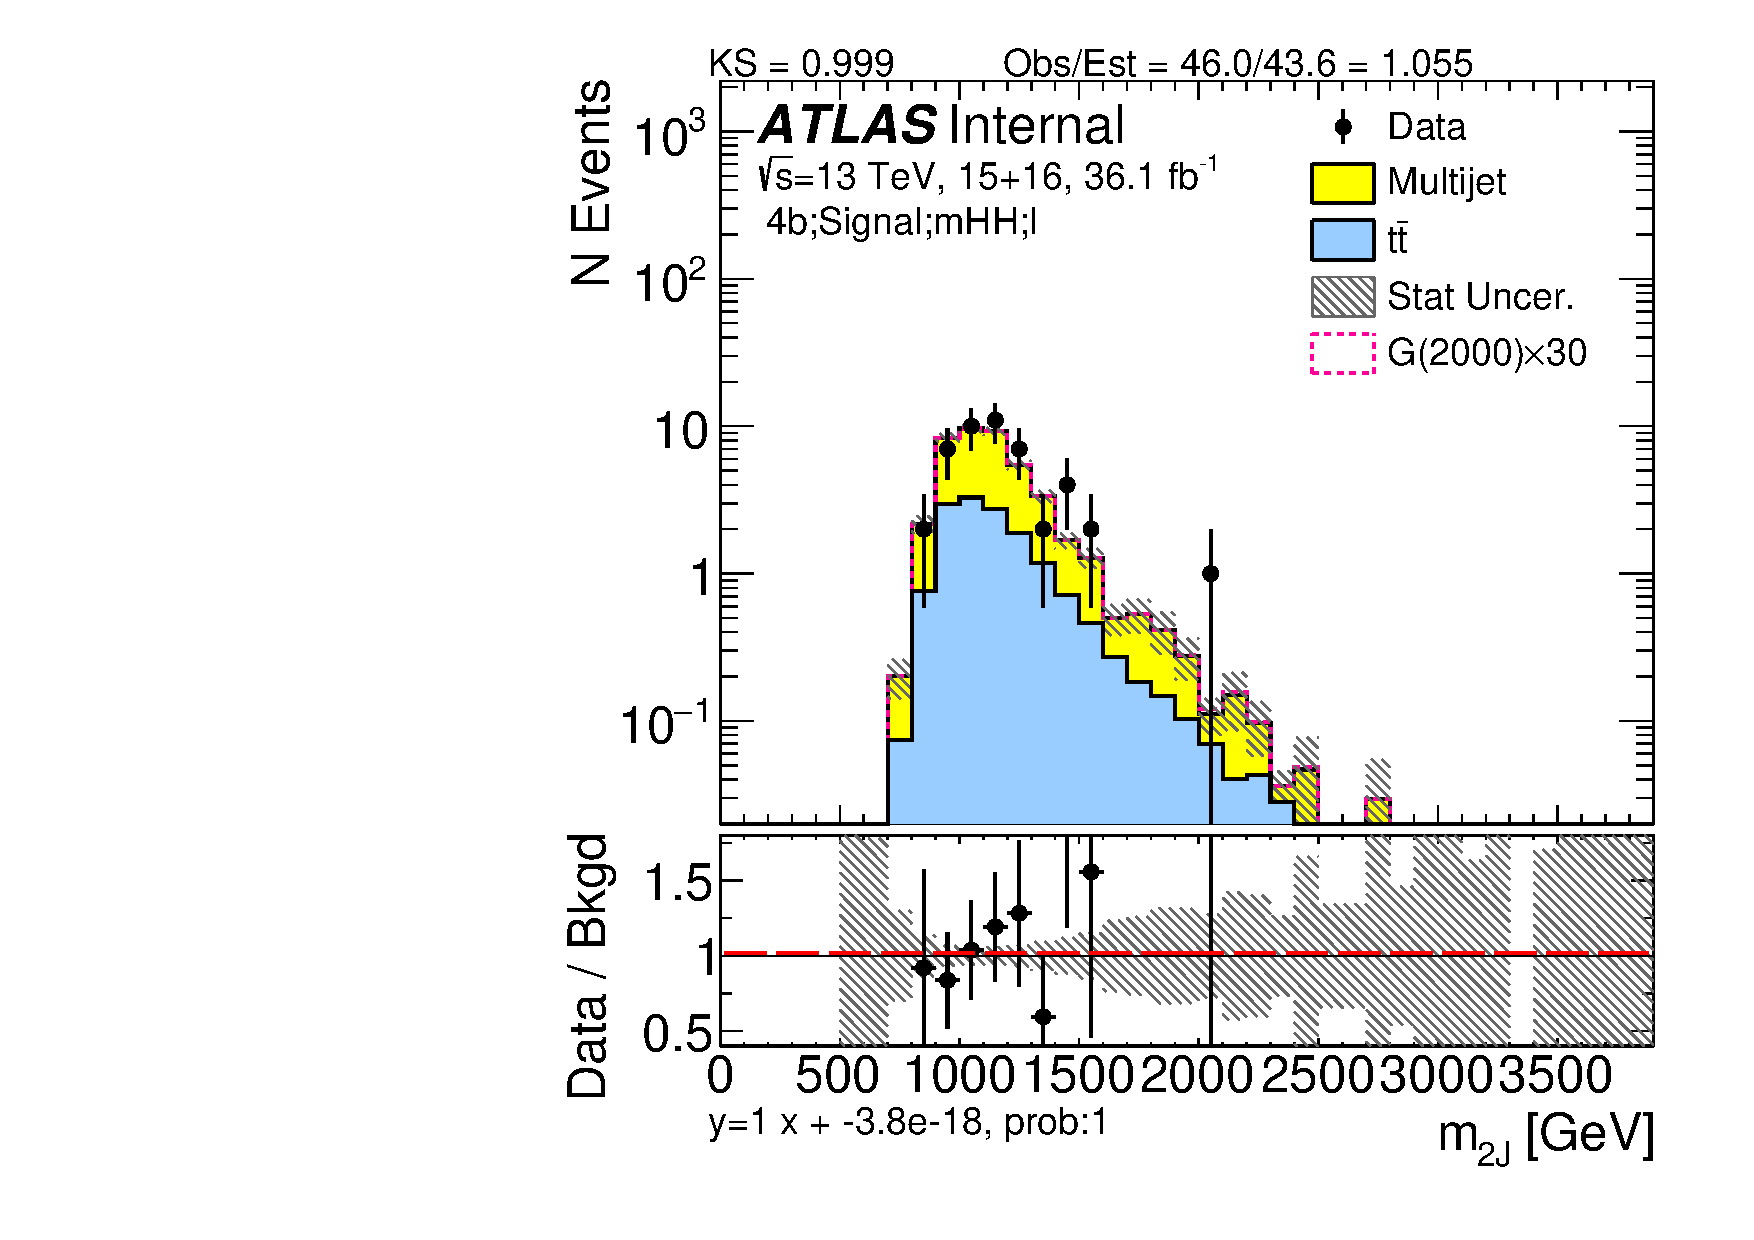
\includegraphics[width=0.45\textwidth,angle=-90]{figures/boosted/TT/Moriond_TT_FourTag_Signal_mHH_l_1.pdf}
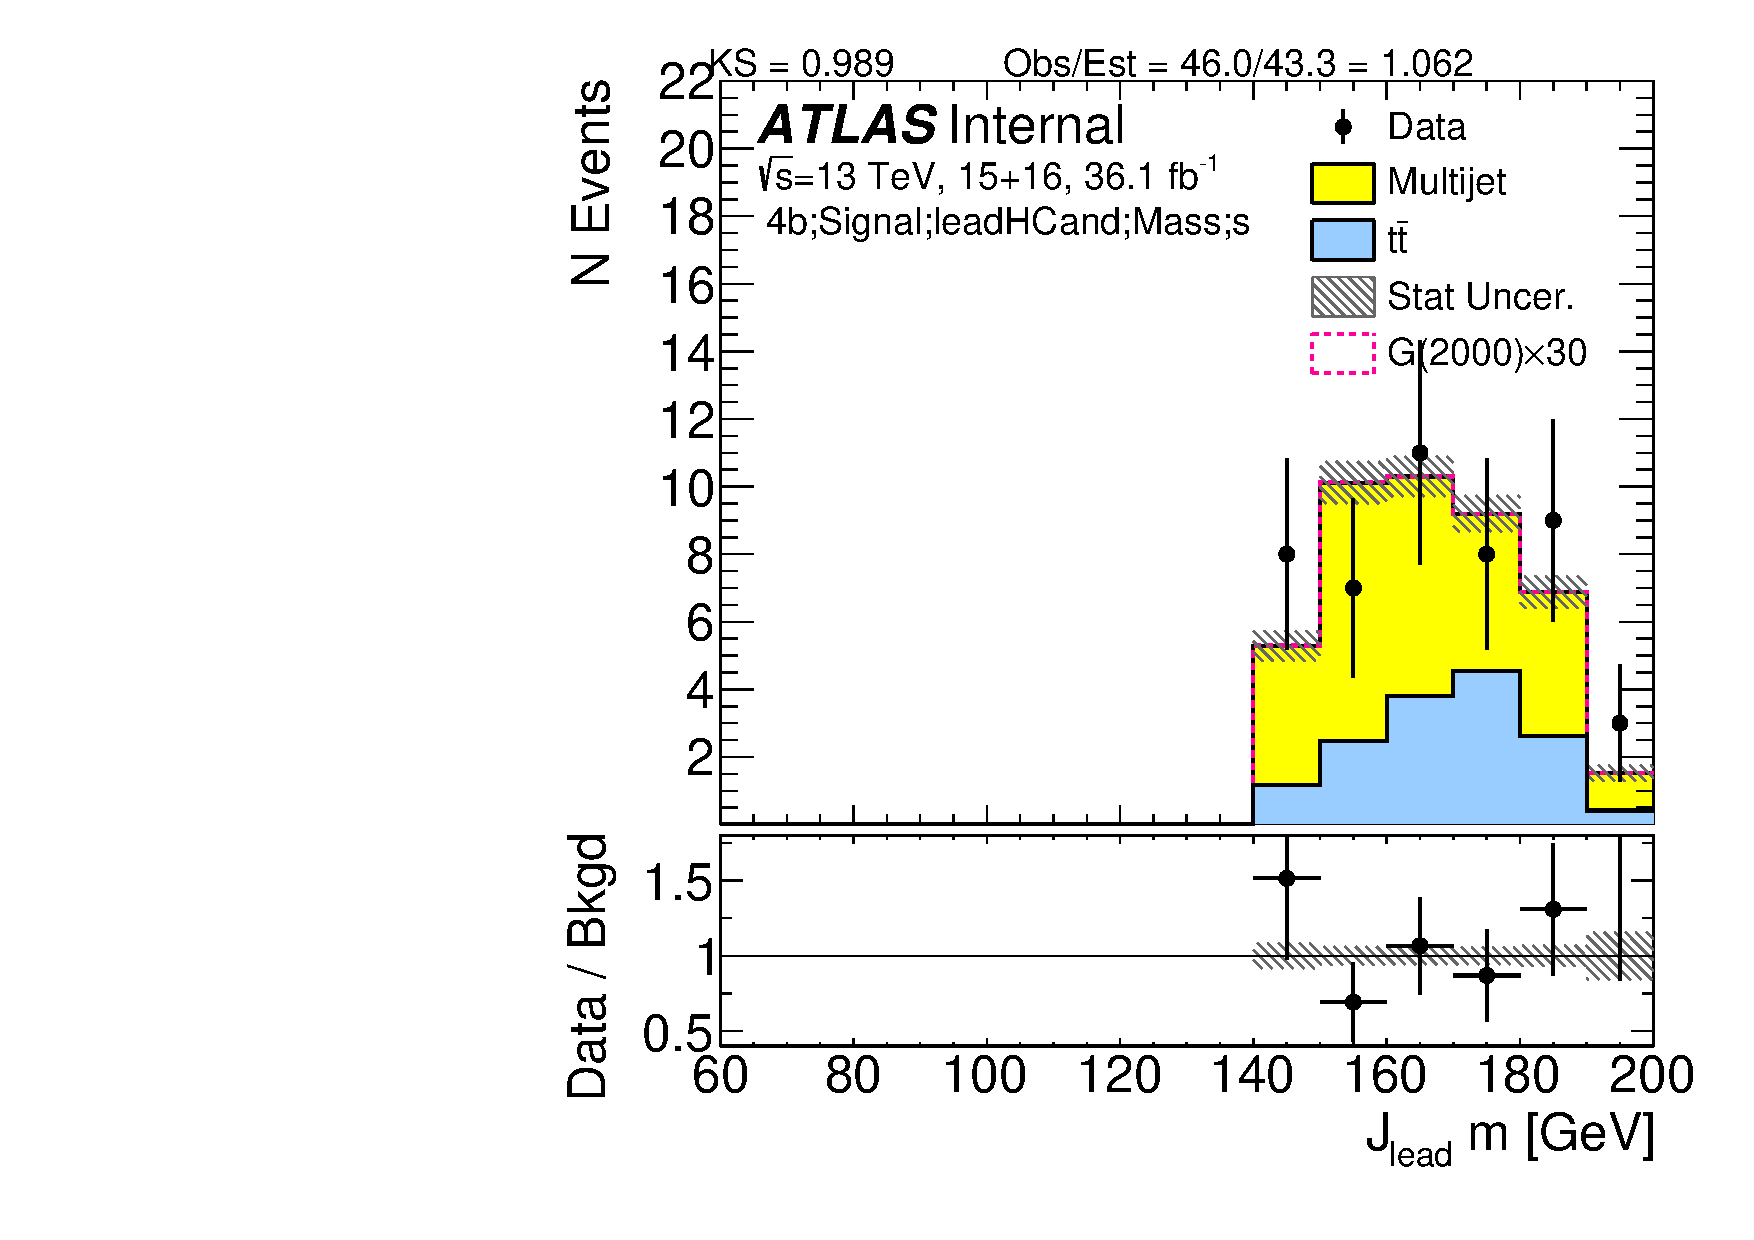
\includegraphics[width=0.45\textwidth,angle=-90]{figures/boosted/TT/Moriond_TT_FourTag_Signal_leadHCand_Mass_s.pdf}\\
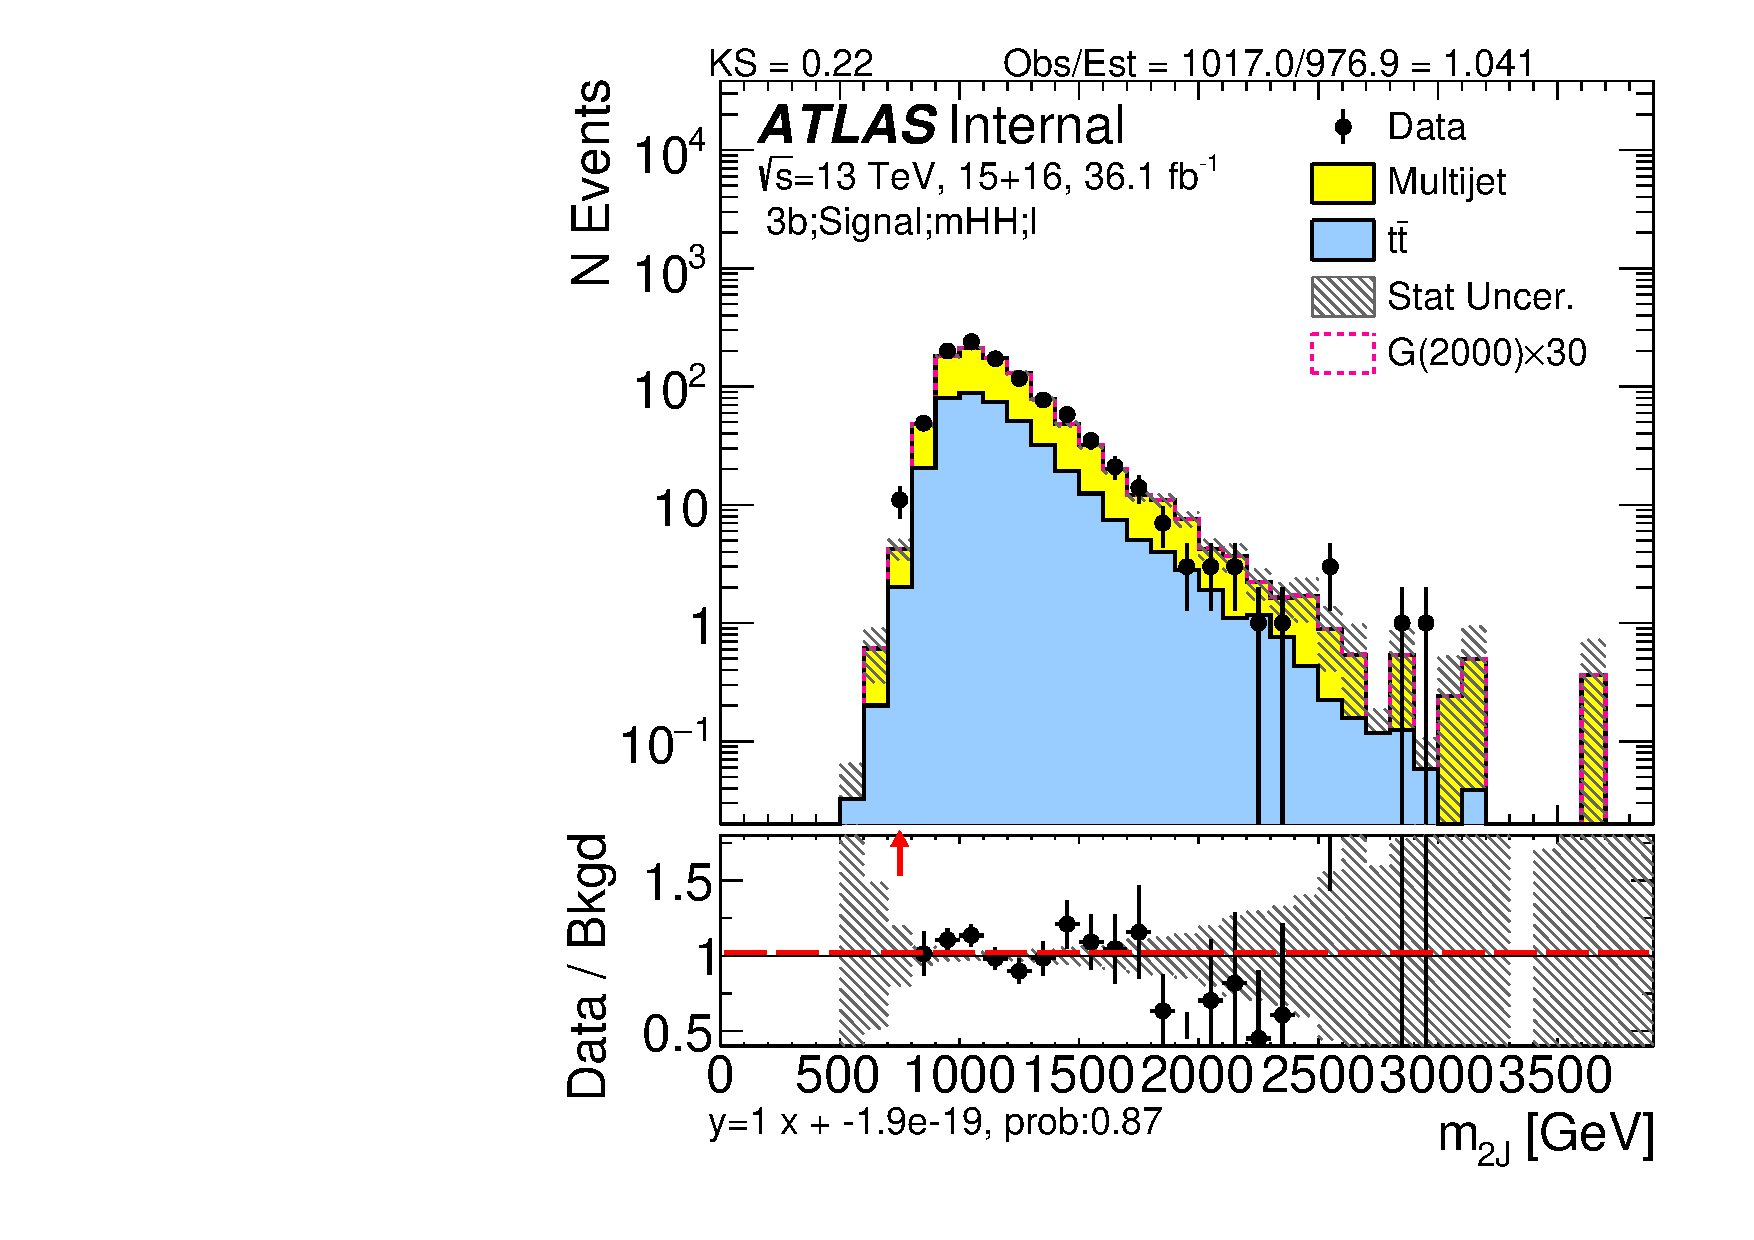
\includegraphics[width=0.45\textwidth,angle=-90]{figures/boosted/TT/Moriond_TT_ThreeTag_Signal_mHH_l_1.pdf}
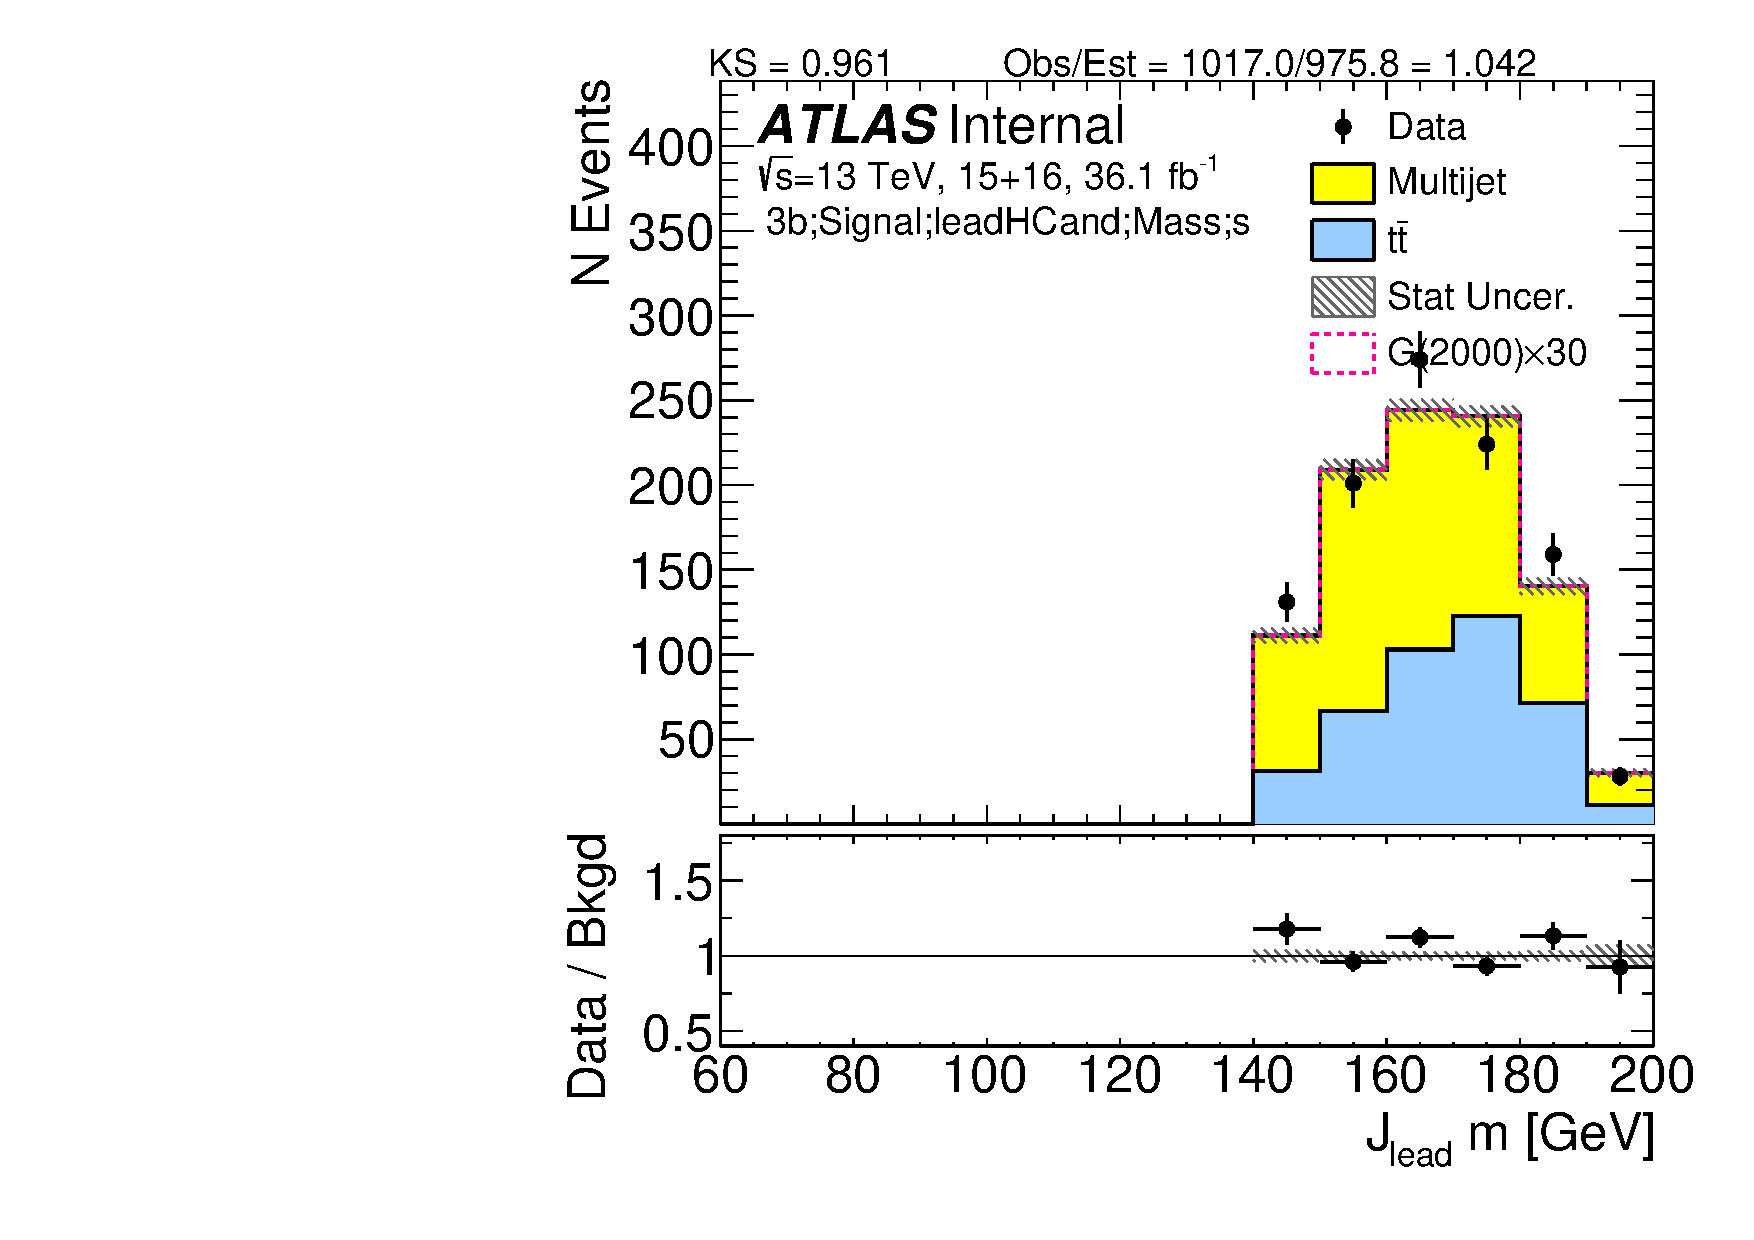
\includegraphics[width=0.45\textwidth,angle=-90]{figures/boosted/TT/Moriond_TT_ThreeTag_Signal_leadHCand_Mass_s.pdf}\\
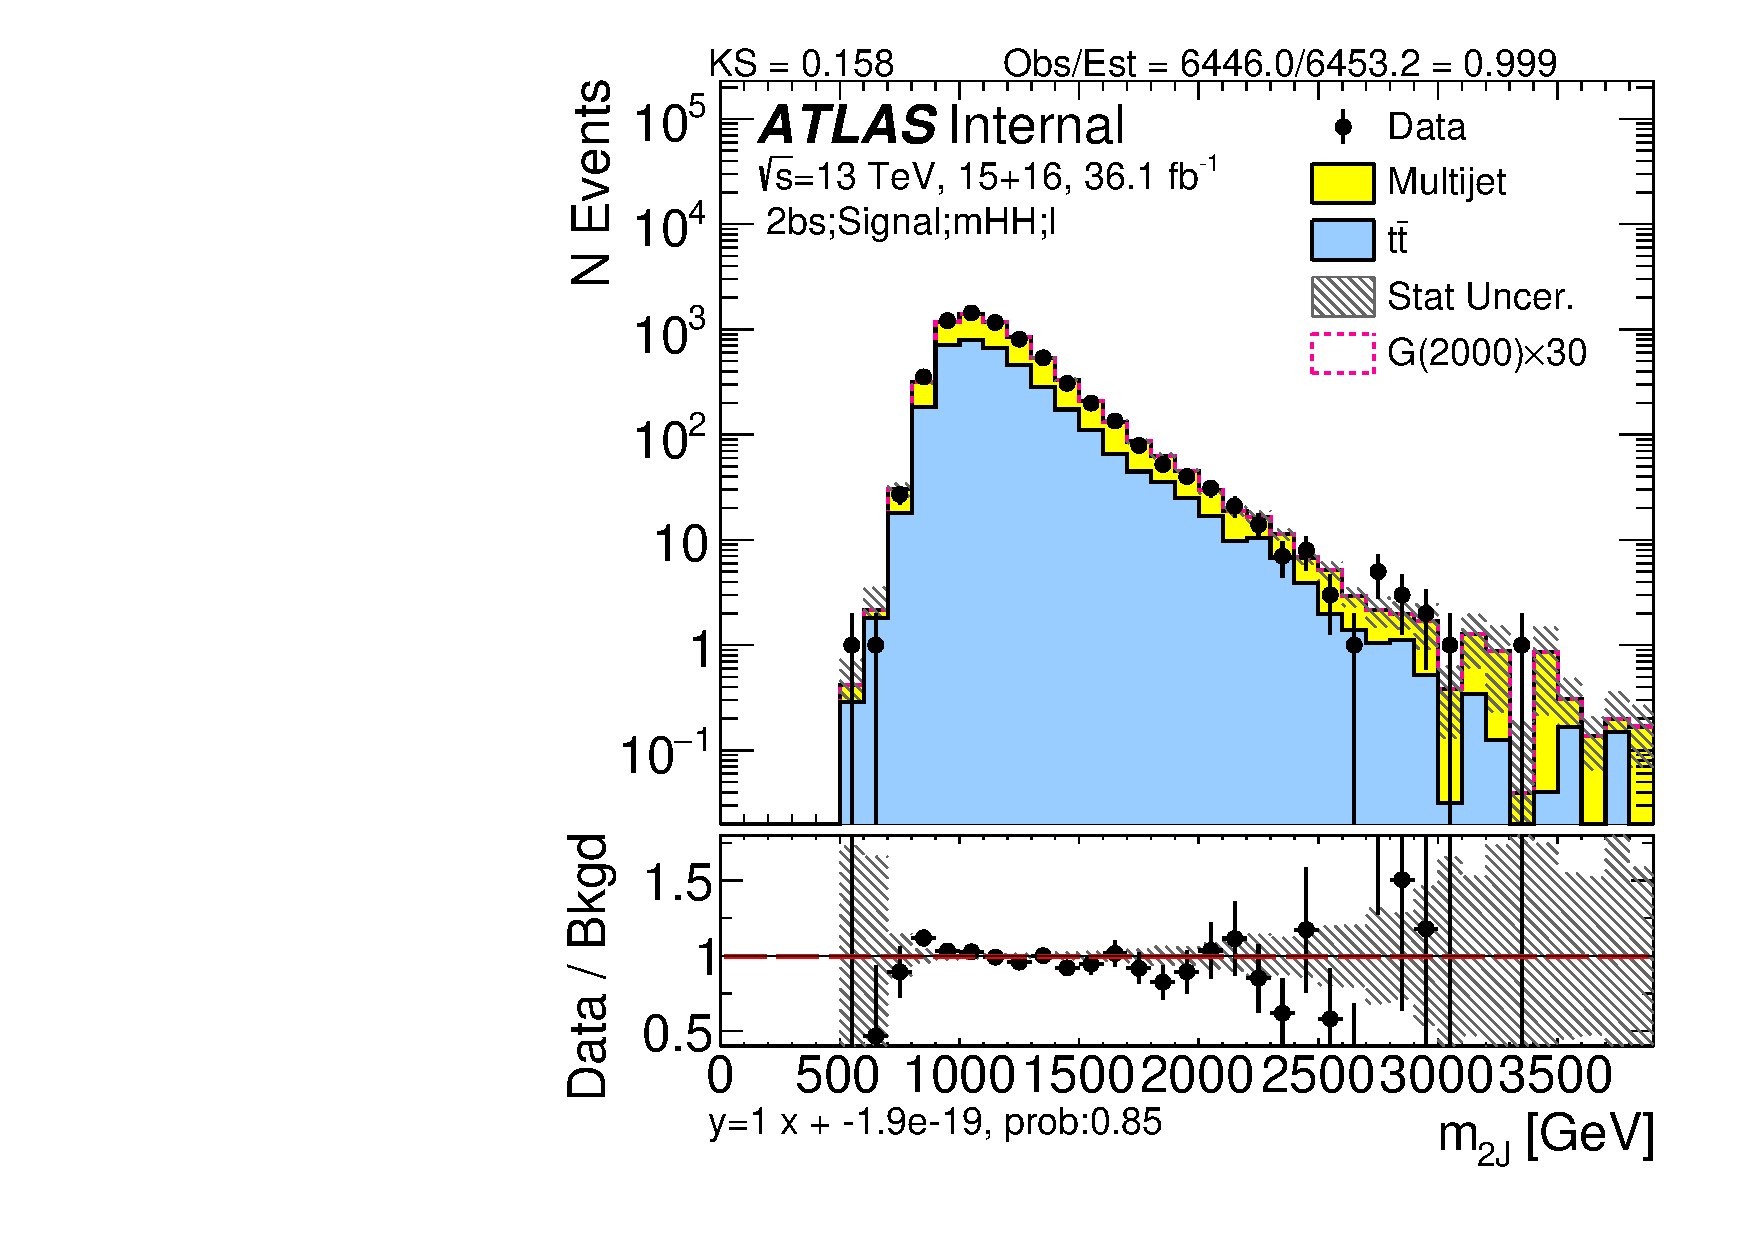
\includegraphics[width=0.45\textwidth,angle=-90]{figures/boosted/TT/Moriond_TT_TwoTag_split_Signal_mHH_l_1.pdf}
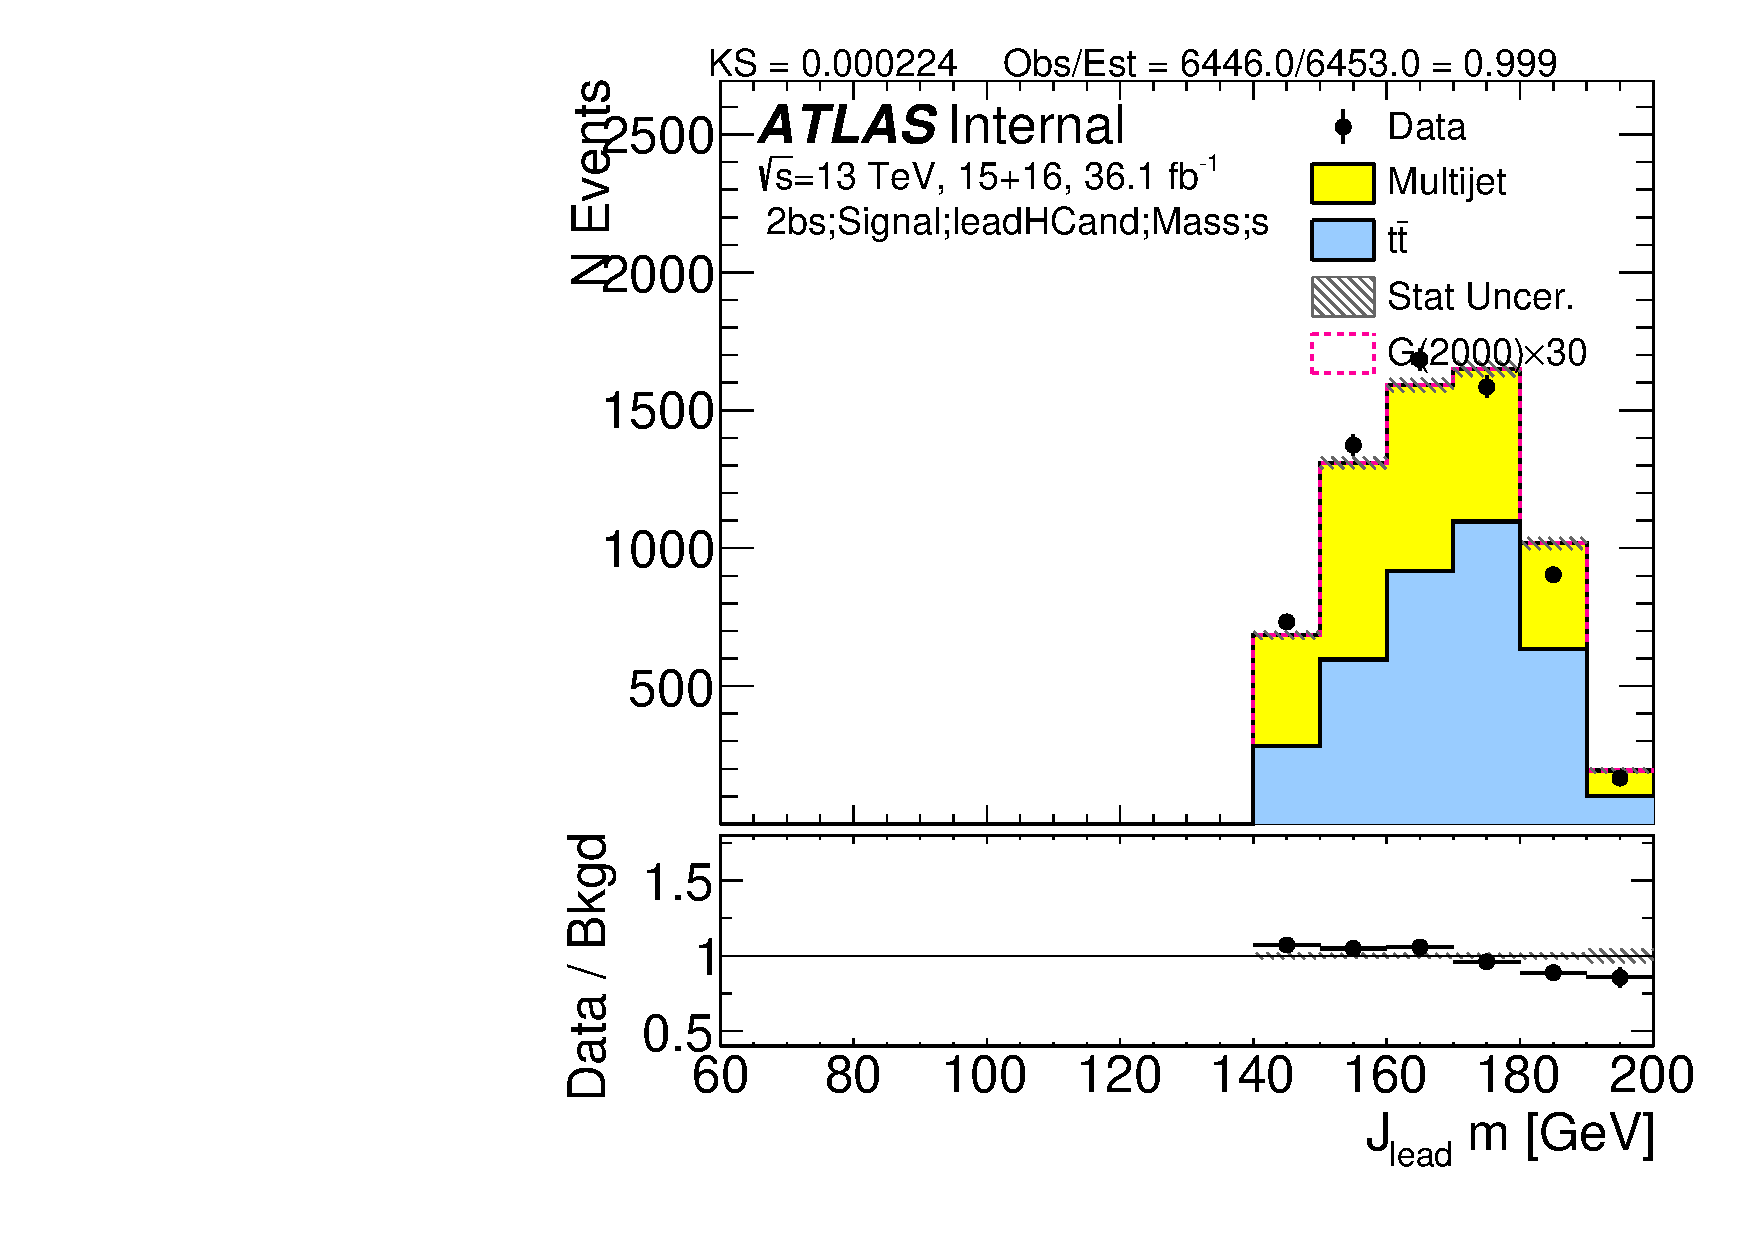
\includegraphics[width=0.45\textwidth,angle=-90]{figures/boosted/TT/Moriond_TT_TwoTag_split_Signal_leadHCand_Mass_s.pdf}\\
\end{center}
\caption{TT signal region distribution of di-jet mass (left column) and leading large-R jet mass (right column) in low mass signal, for $4b$ (top row), $3b$(middle row) and $2b$ split (bottom row). The plots are with only statistical uncertainty.}
\label{CRSB:TTSR_Distribution}
\end{figure}



\clearpage
\subsubsection{Uncertainty on the shape of the \ttbar\ jet mass in the $4/3b$ signal region}
\label{sec:unc-shape-ttbar-in-sr}

%In a similar method as stated in the previous section, the shape uncertainty of the signal region dijet mass in \ttbar\ events due to b-tagging or c-rejection is conservatively estimated by comparing the 0b, 1b, 2b, 3b, 4b distributions to the nominal 3b/4b shapes. Figure~\ref{ttbar-shapes-signal} shows the \ttbar\ leading jet and dijet mass distributions in the signal region, all normalized to the predicted number of events in the signal region from the simultaneous fit for \alphatt\ in the sideband.  
%All shapes are comparable within statistical uncertainties.  The difference in shape between the 2b and 3b distributions is taken as the \ttbar\ shape systematic in the signal region.  These shapes are further validated in data in a \ttbar-enriched region, as discussed in Section~\ref{sec:boosted-ttbar}.

%%\paragraph{}
Because the 4/$3b$ \ttbar\ MJJ distribution is extremely statistically limited, the 4/$3b$ shape is used to predict the final \ttbar\ background shape in the $2bs$ signal region. In order to estimate the possible shape uncertainty, the $2bs$ and $3b$ sideband shapes are compared in Figure~\ref{fig:ttbar-shapes-signal} (after being normalized to the same area).  The $2bs$ is used as there are not sufficient $4b$ statistics to asses the comparison quality. In order to avoid large statistical uncertainties, the distributions of the $3b$ and $2b$ are smoothed. The ratio of the two smoothed distributions is taken as the shape systematic. We then use this function to apply a bin-by-bin scaling of the \ttbar\ background prediction in the signal region, maintaining the same normalization given by nominal $t\bar{t}$ normalization prediction.

\begin{figure}[htbp!]
\begin{center} 
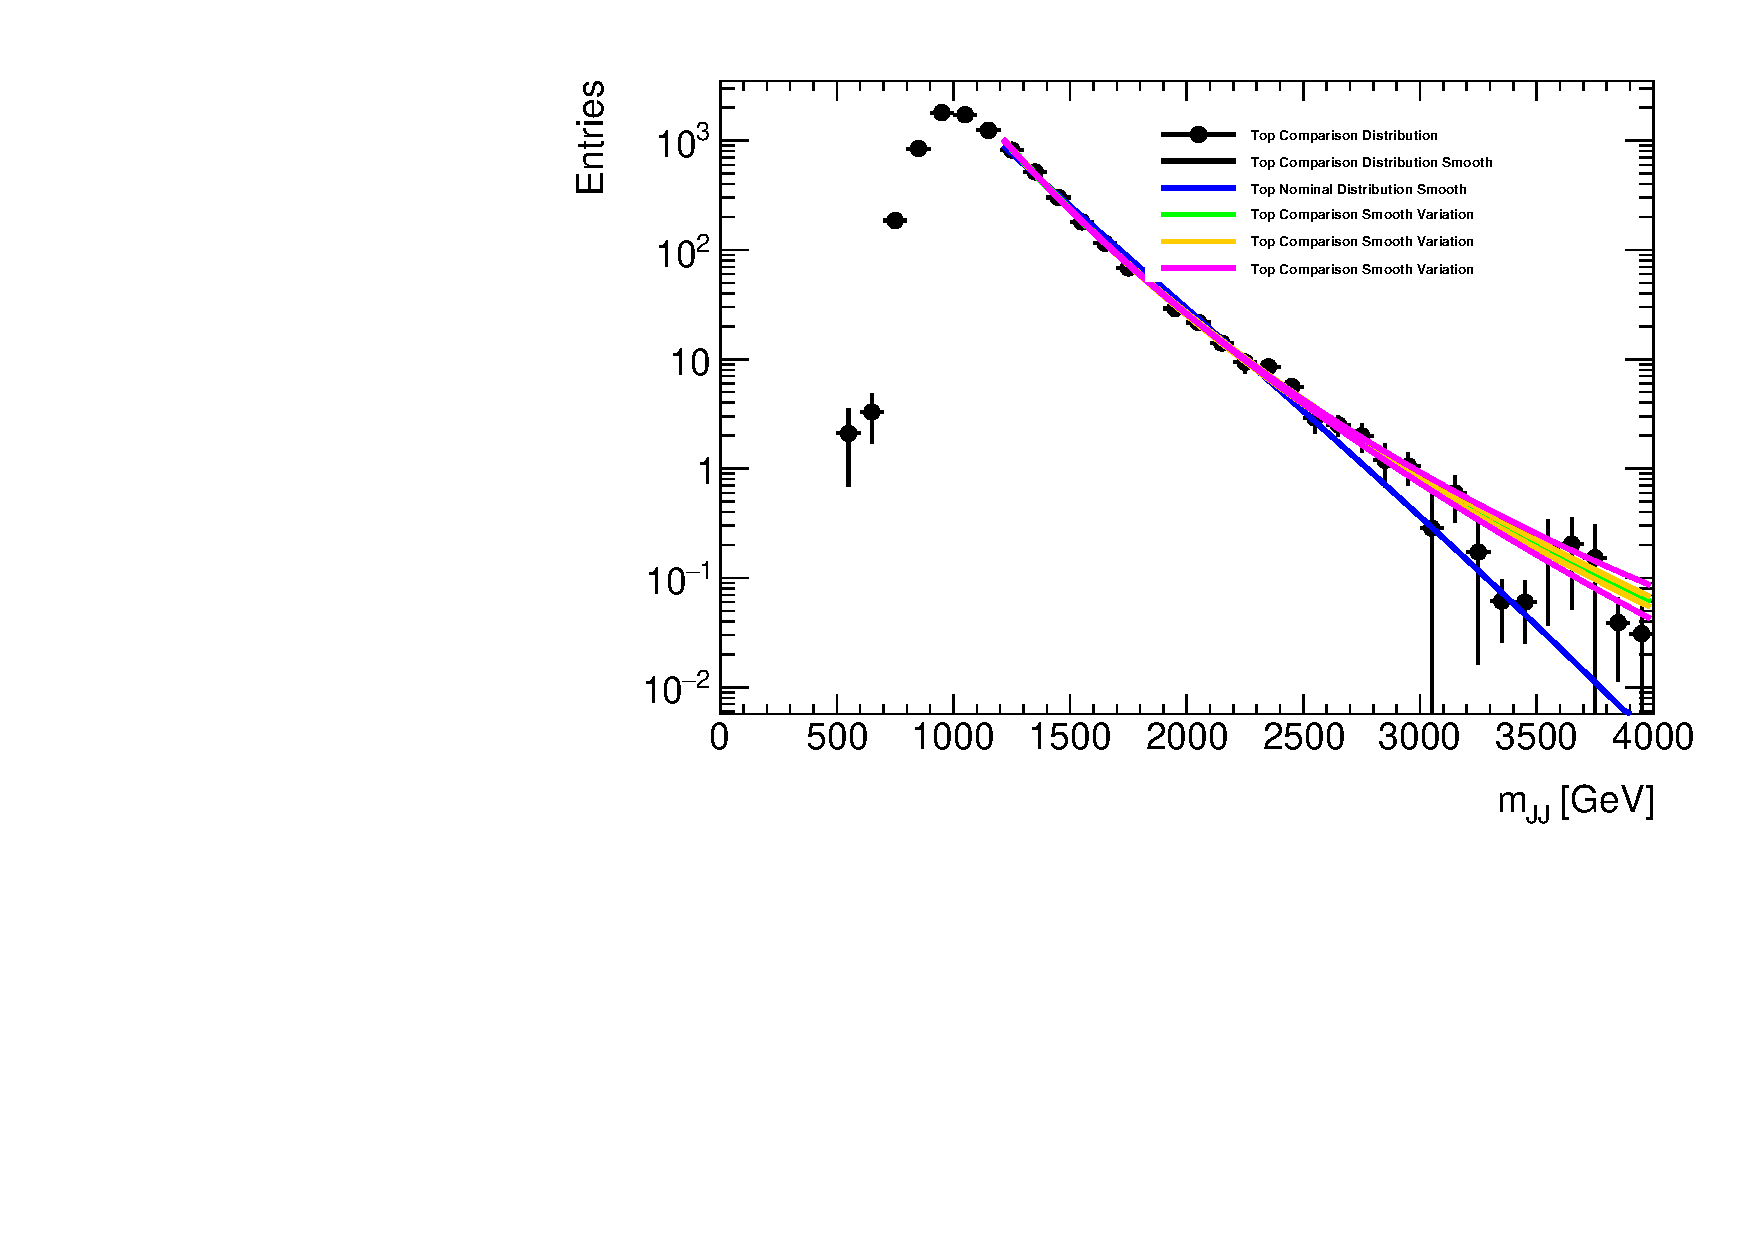
\includegraphics[width=0.48\textwidth,angle=-90]{figures/boosted/Syst_Smooth/TopShapeSRSysfitSmooth_sig33_comp22.pdf}
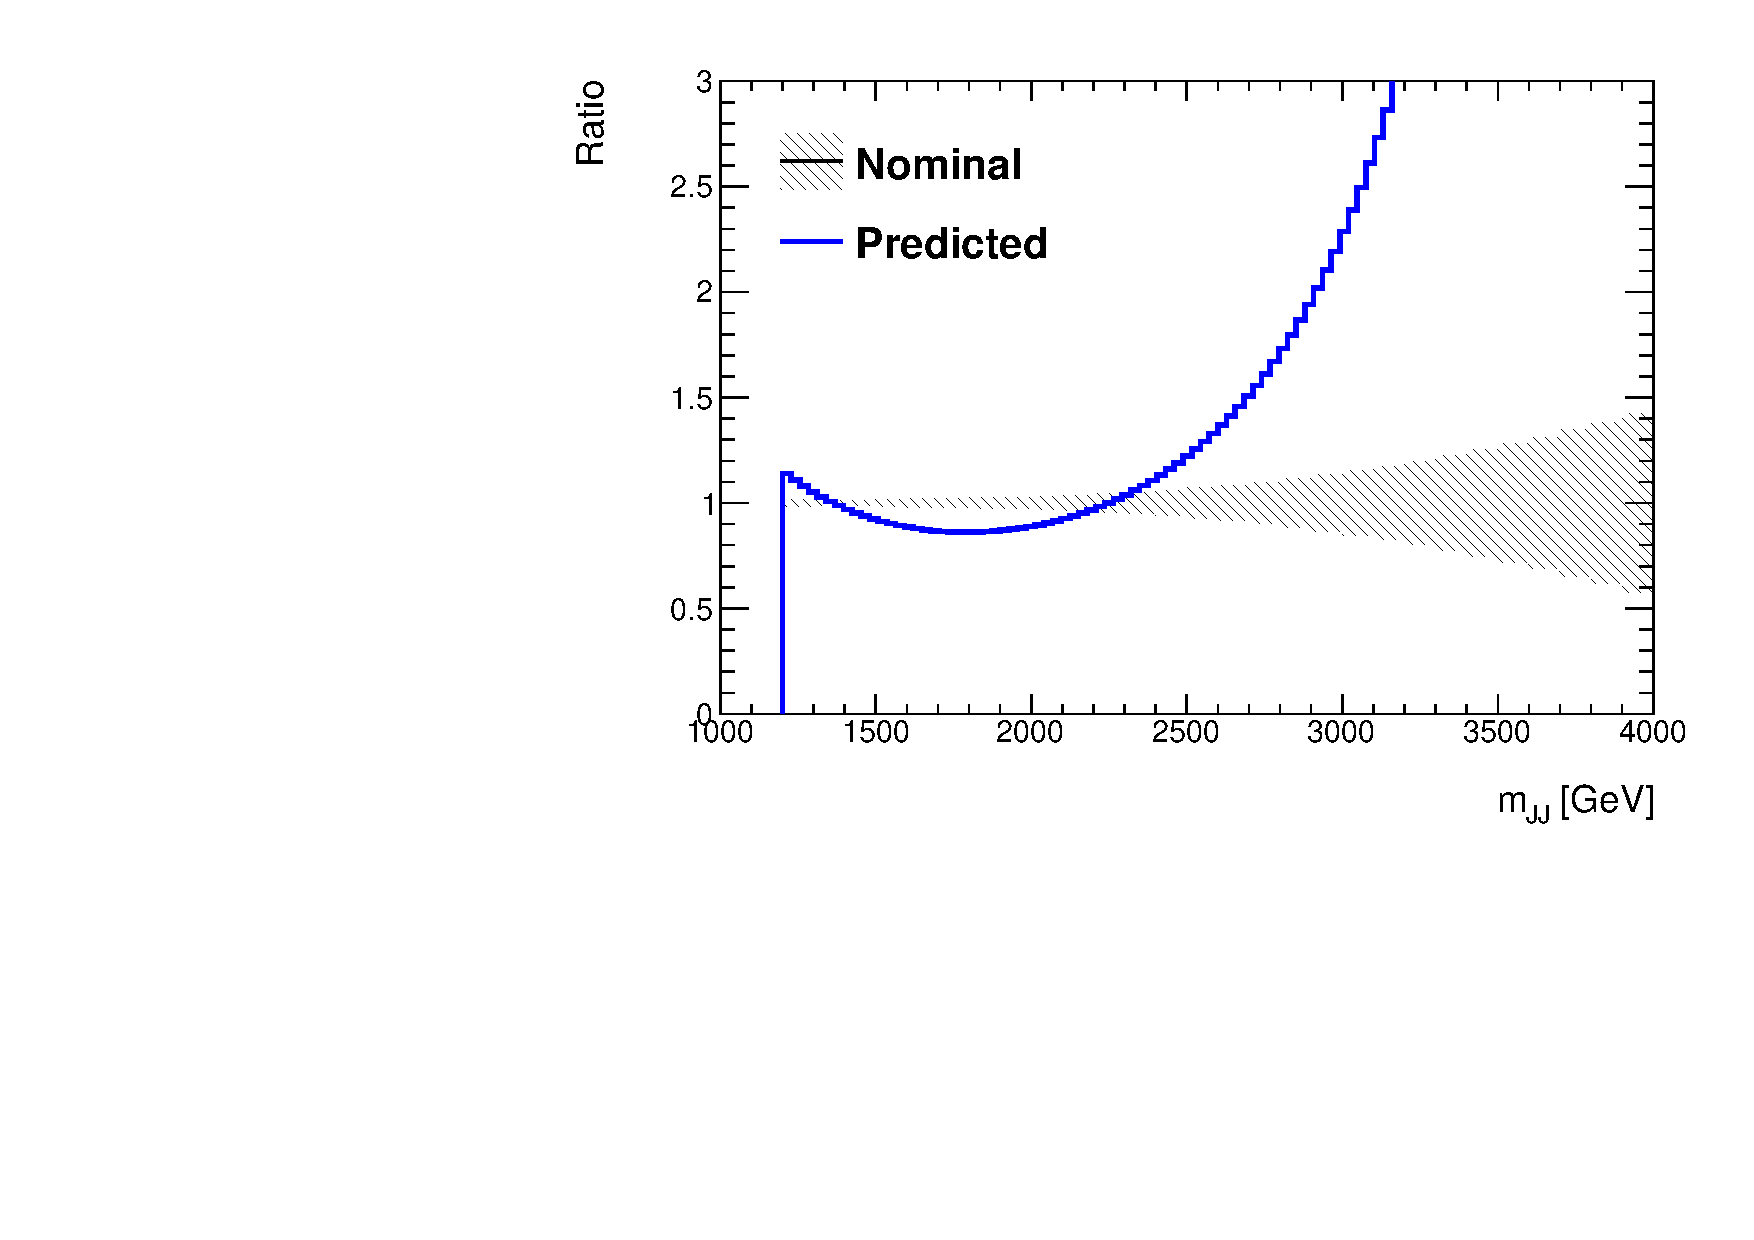
\includegraphics[width=0.48\textwidth,angle=-90]{figures/boosted/Syst_Smooth/TopShapeSRSysfitSmooth_sig33_comp22_ratio.pdf}
\caption{(left)  Shape of the \ttbar\ di-\largeR-jet mass in the sideband region,
comparing the $3b$ shape with that of the $2b$, in order to asses the systematic effect of additional $b$-tags changing the dijet mass distribution.  The $m_{JJ}$ distributions is shown on the left, and the ratio of $3b$ to $2b$ distributions on the right.}
\label{fig:ttbar-shapes-signal}
\end{center}
\end{figure}

%The same method is applied to for the \ttbar\ shape uncertainty for the scaled dijet mass distribution.  The ratio of the $4b$ to $3b$ shape, as well as the linear fits and variations used to determine the shape uncertainty can be found in Figure~\ref{fig:ttbar-shapes-signal-scaled}.
%
%\begin{figure}[htbp!]
%\begin{center} 
%%%\includegraphics[width=0.48\textwidth,angle=-90]{figures/boosted/background/DiJetMassPrime/topshape_44.pdf}
%\caption{The ratio of $4b$ to $3b$ shapes of the \ttbar\ scaled di-\largeR-jet mass in the signal region, with a linear fit to the ratio.  The same fit with negative slope is also shown on the figure.  \textbf{TO BE UPDATED} }
%\label{fig:ttbar-shapes-signal-scaled}
%\end{center}
%\end{figure}

\clearpage
\subsubsection{Uncertainty on the shape of the $1/2b$ QCD distribution in the signal region}
\label{unc-shape-qcd-in-sr}

%%\paragraph{}
As shown in Figures~\ref{fig:boosted-4b-control-ak10-system} and~\ref{fig:boosted-3b-control-ak10-system}, the shape distribution of the total predicted background using the scaled $1/2b$ QCD sample was found to be in good agreement with the $4b$, $3b$, and $2bs$ data in the control region.  However due to the low statistics in the data in the control region, the comparison is performed by first smoothing the $1/2b$, and the $4/3/2bs$ distributions. The ratio of the smoothed $1/2b$ distributions to that of the smoothed $4/3/2bs$ distributions is taken as the shape systematic. This function is then used to apply a bin-by-bin scaling of the QCD background prediction in the signal region, maintaining the same normalization given by \muqcd.  The CR distributions and the smoothing fit ratios can be found in Figure~\ref{fig:qcd_shape_fit}. This systematics is further split into two parts: one below 2000 \GeV and the other above 2000 \GeV, to ensure the low and high mass shape variation post-fit pulls can vary independently. It should be noted, that this uncertainty is used for both the dijet mass, and the scaled dijet mass distribution, and the correction to to scaling is expected to be small relative to the dijet mass. 

\begin{figure}[htbp!]
\begin{center}
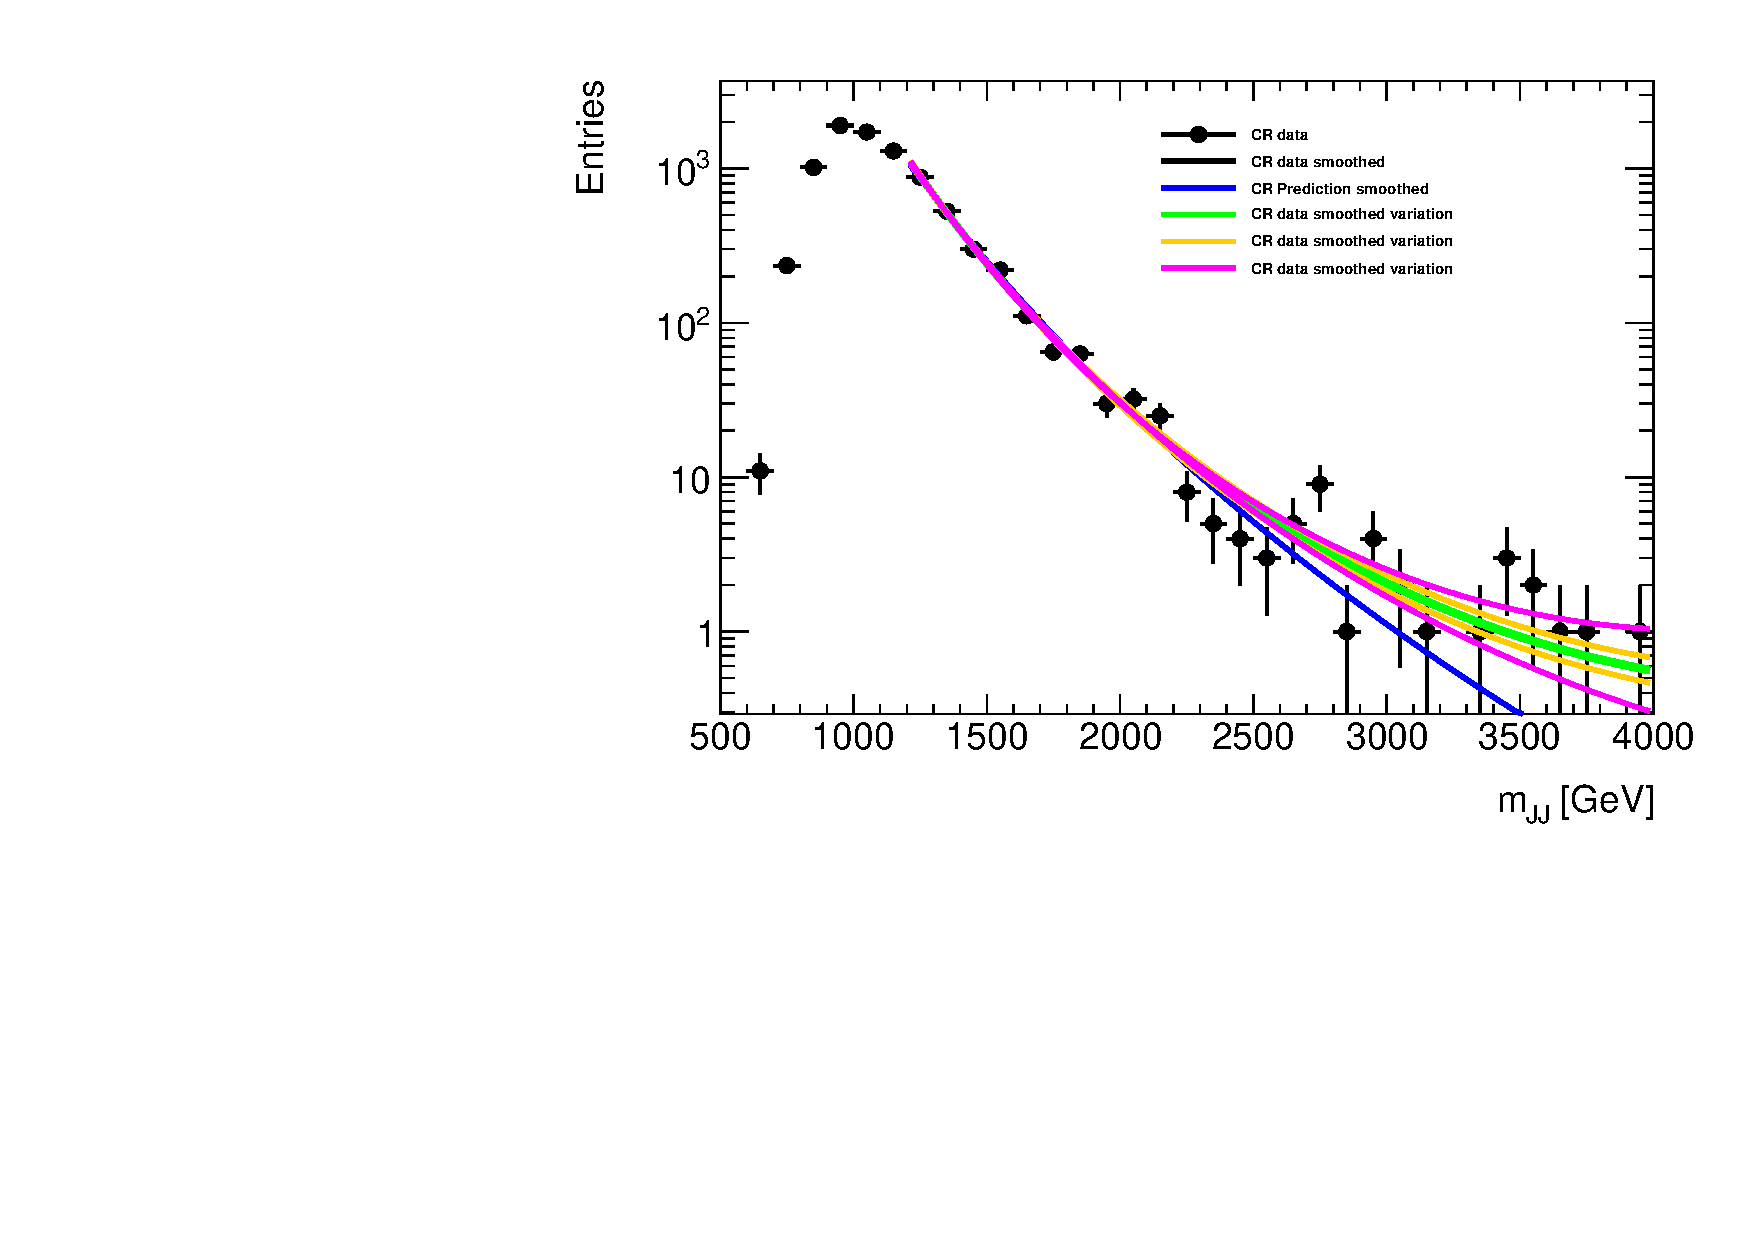
\includegraphics[width=0.4\textwidth,angle=-90]{figures/boosted/Syst_Shape/QCDSysfitSmooth_22.pdf}
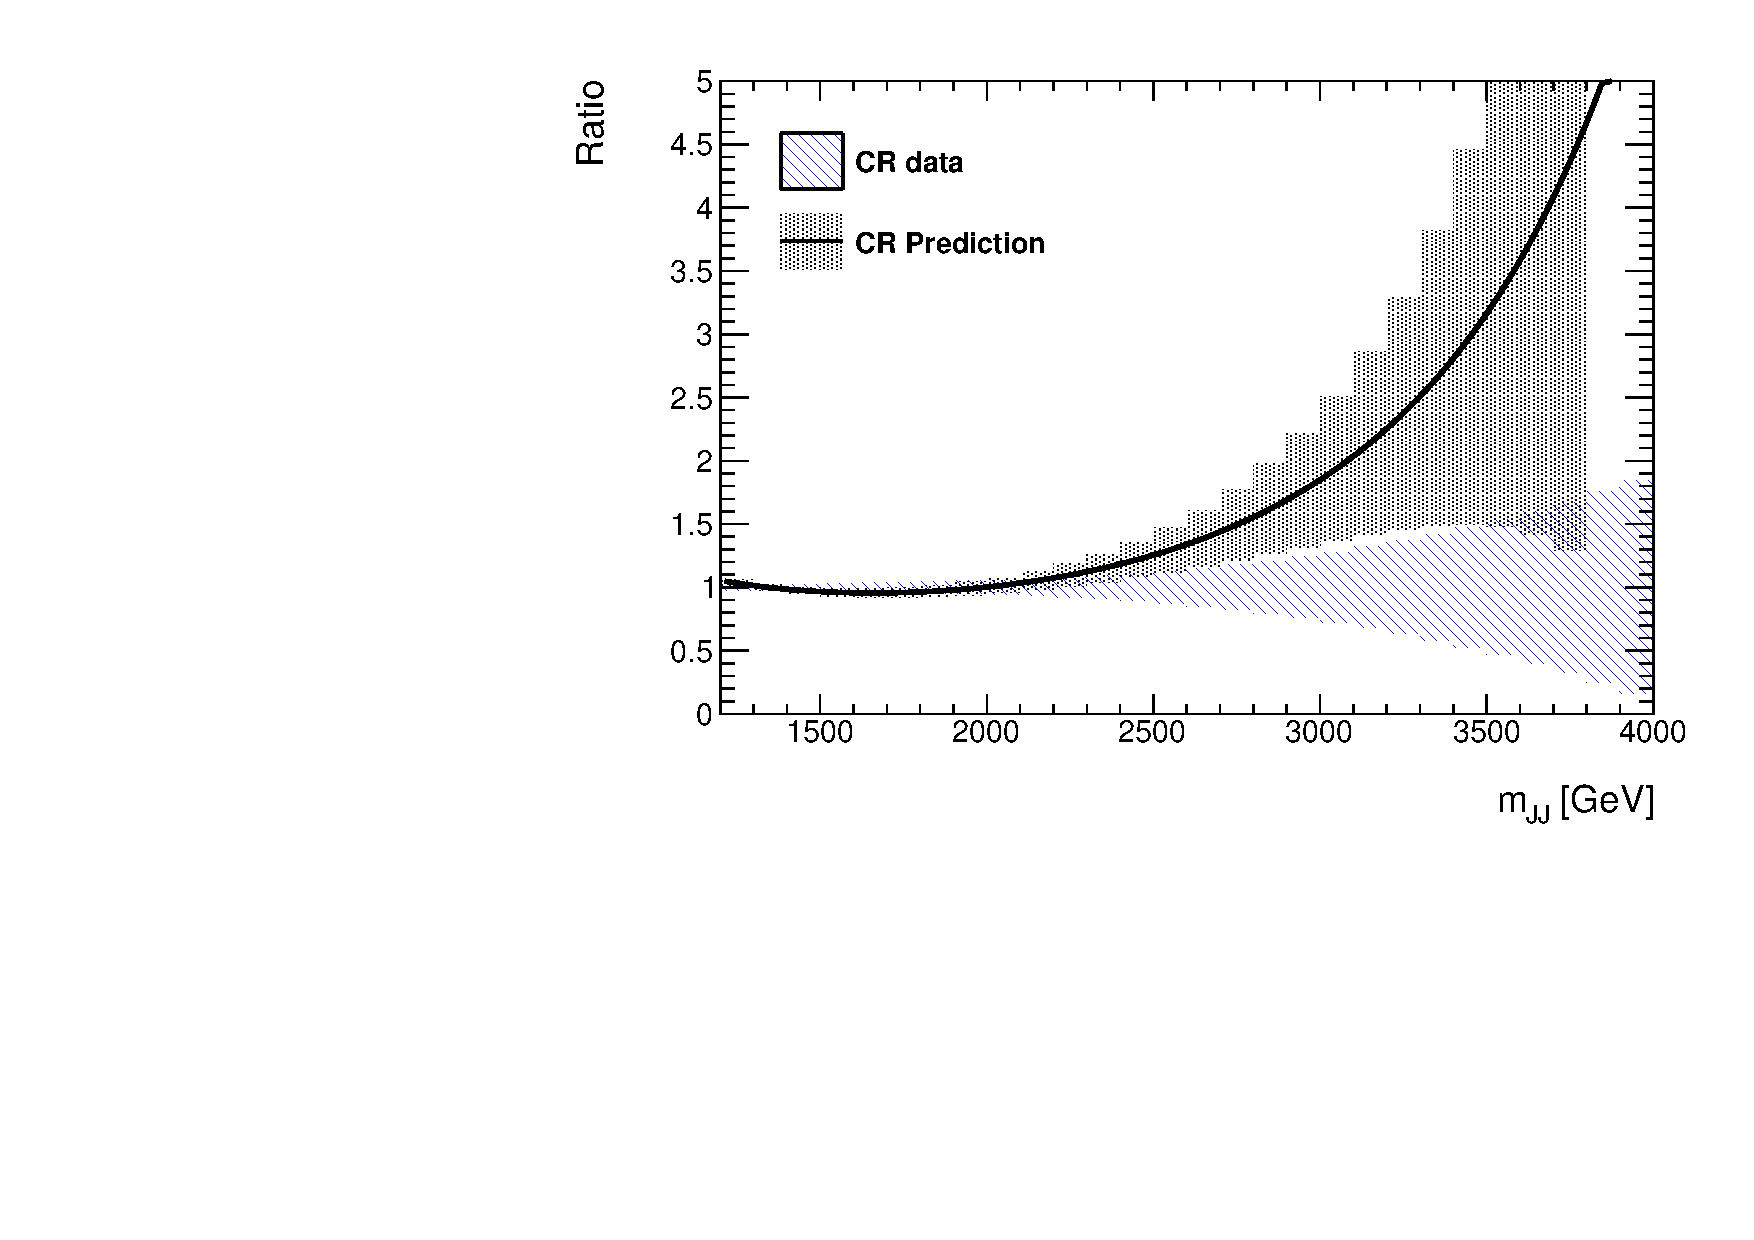
\includegraphics[width=0.4\textwidth,angle=-90]{figures/boosted/Syst_Shape/QCDSysfitSmooth_ratio_22.pdf} \\
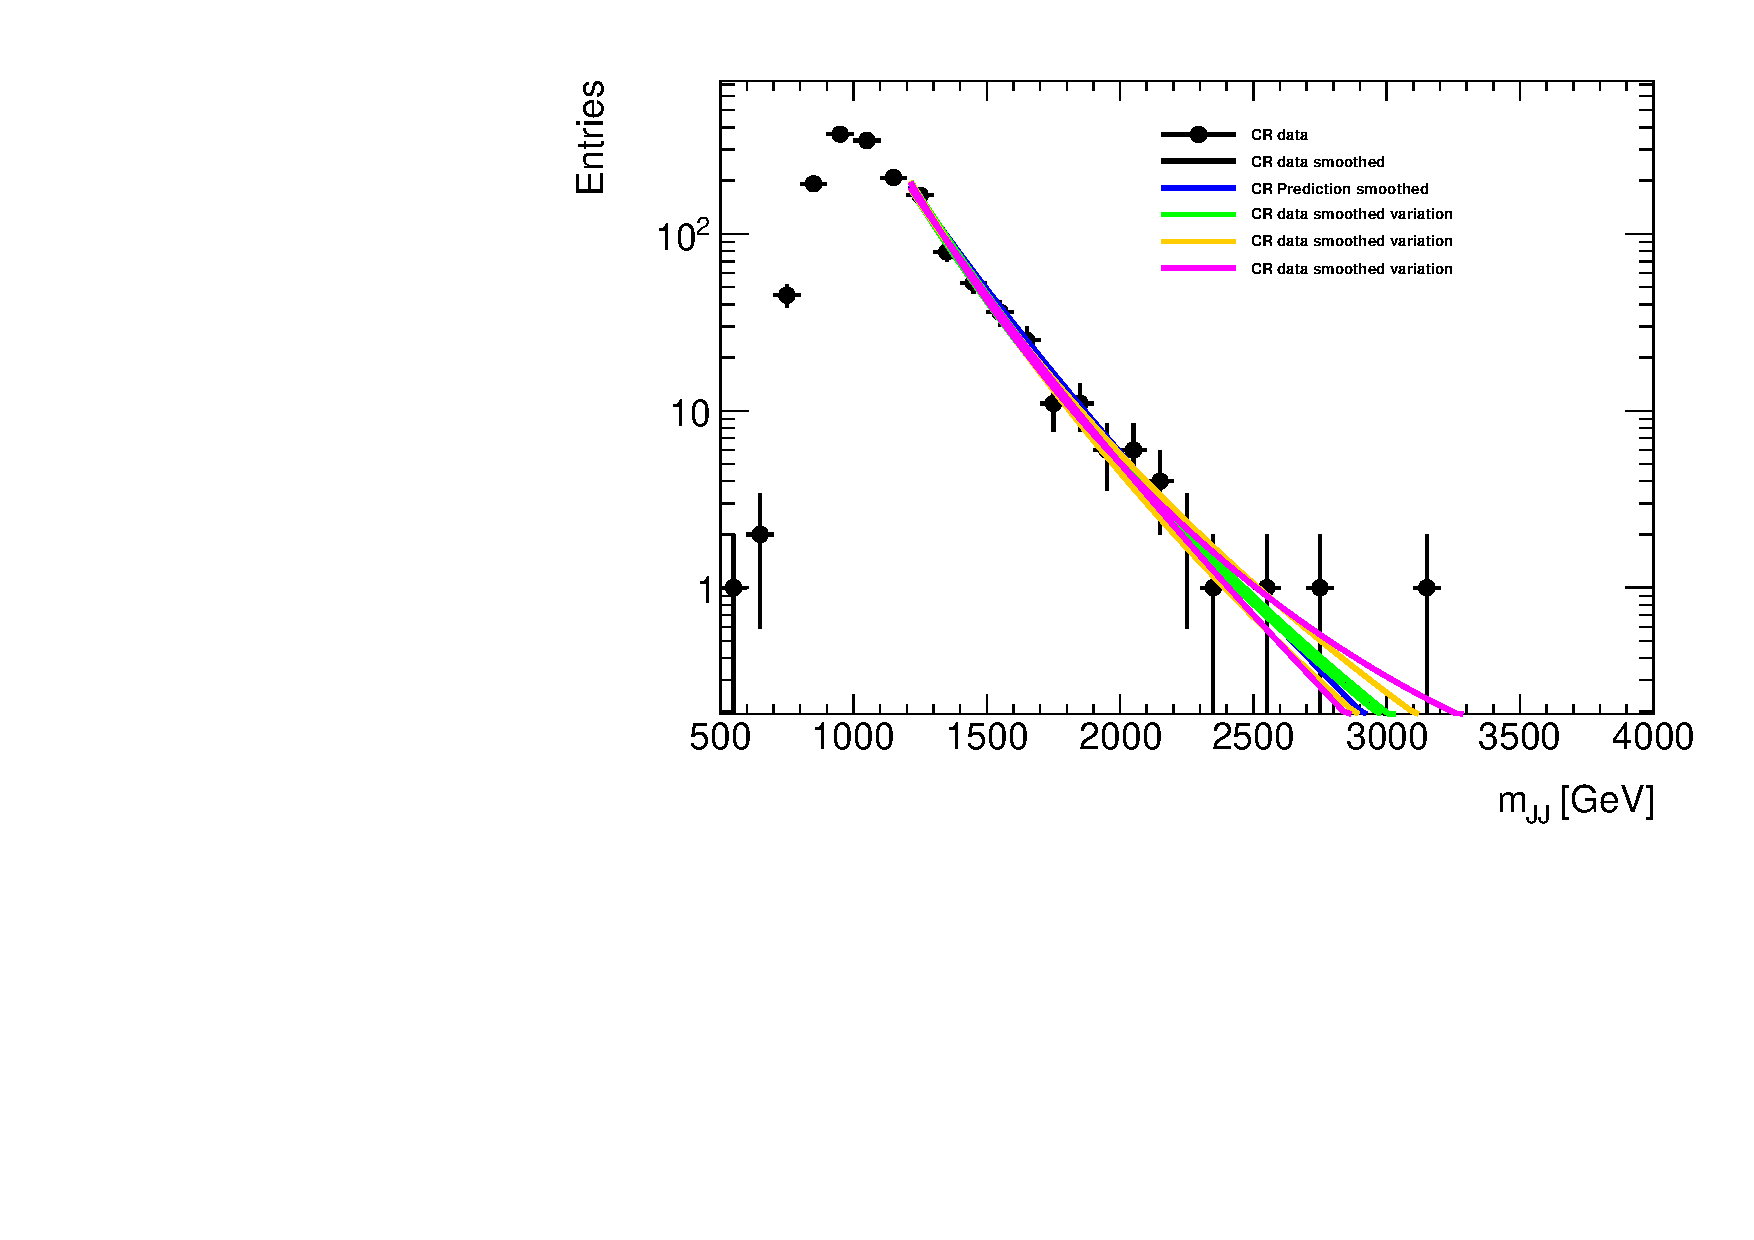
\includegraphics[width=0.4\textwidth,angle=-90]{figures/boosted/Syst_Shape/QCDSysfitSmooth_33.pdf}
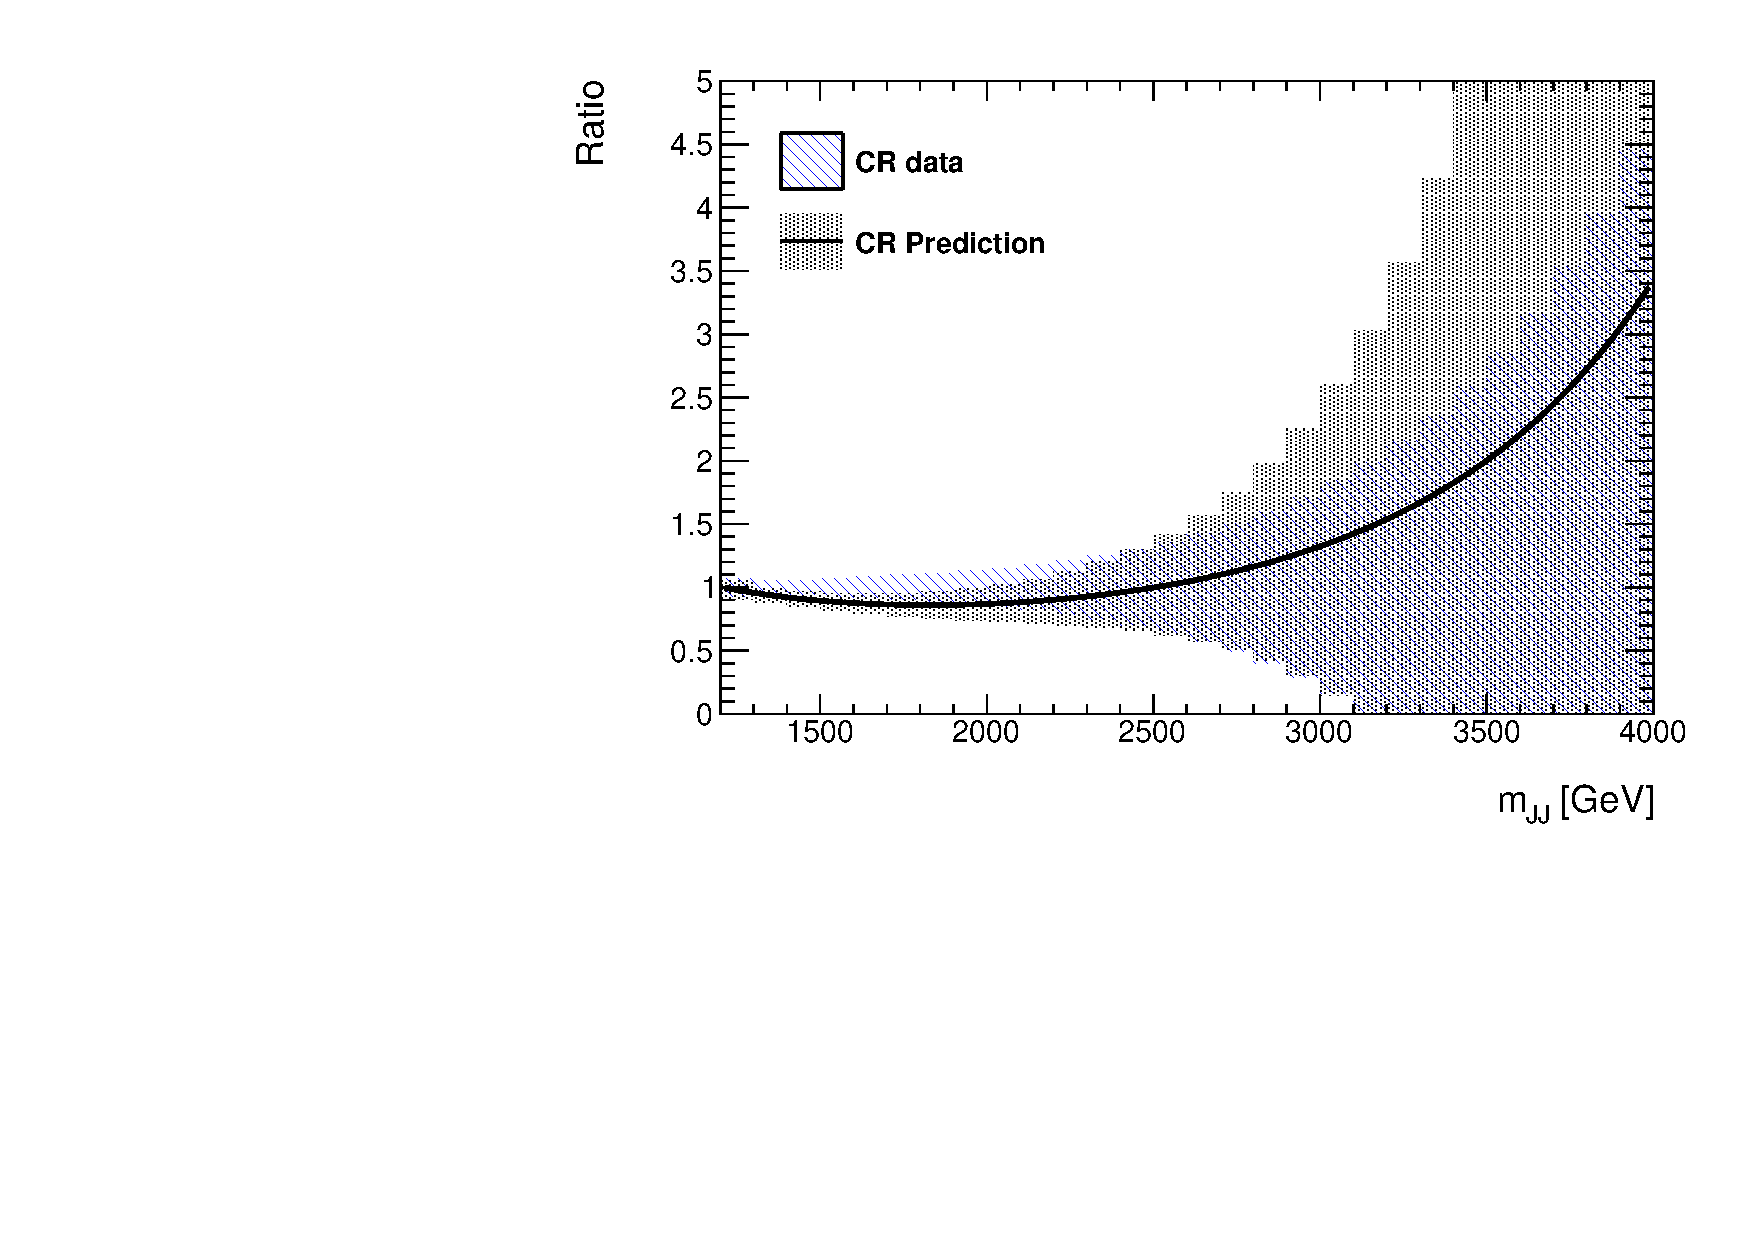
\includegraphics[width=0.4\textwidth,angle=-90]{figures/boosted/Syst_Shape/QCDSysfitSmooth_ratio_33.pdf} \\
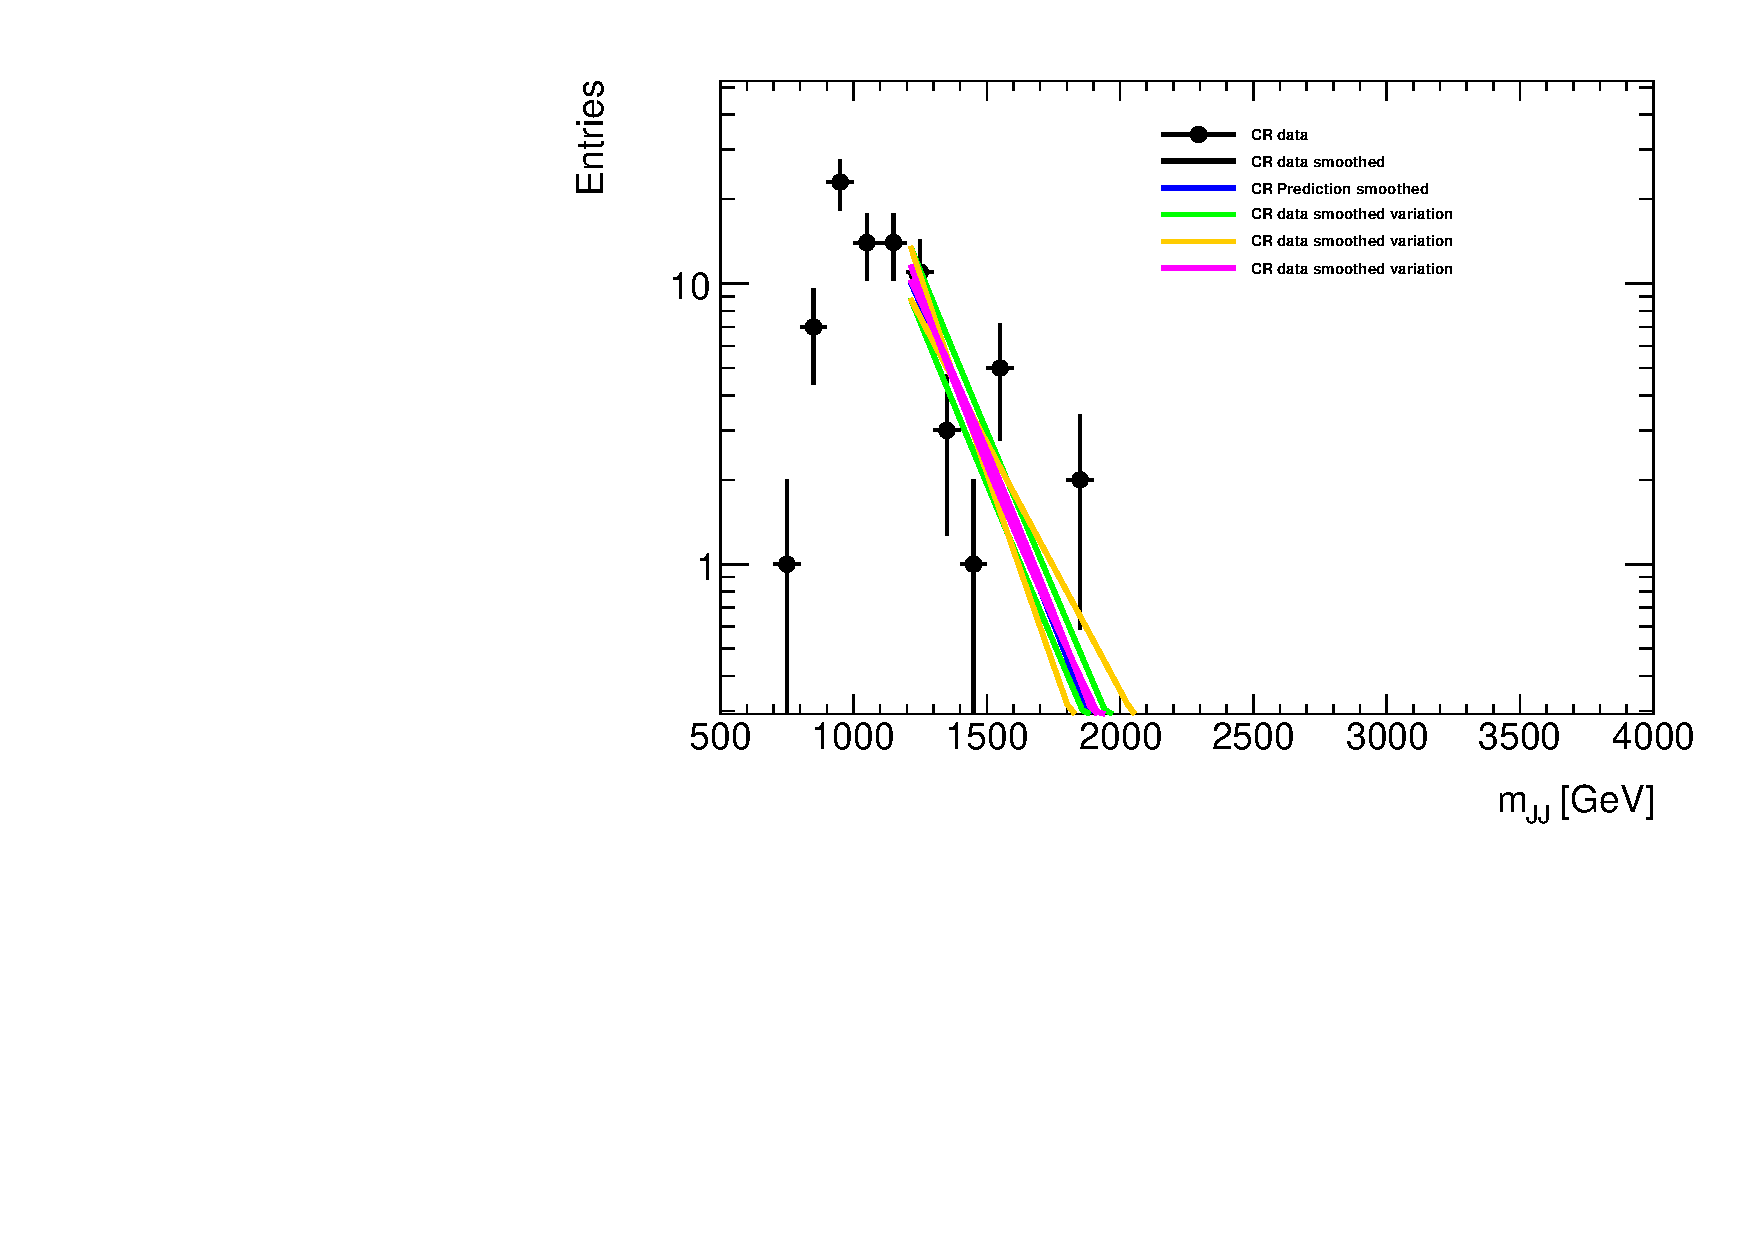
\includegraphics[width=0.4\textwidth,angle=-90]{figures/boosted/Syst_Shape/QCDSysfitSmooth_44.pdf}
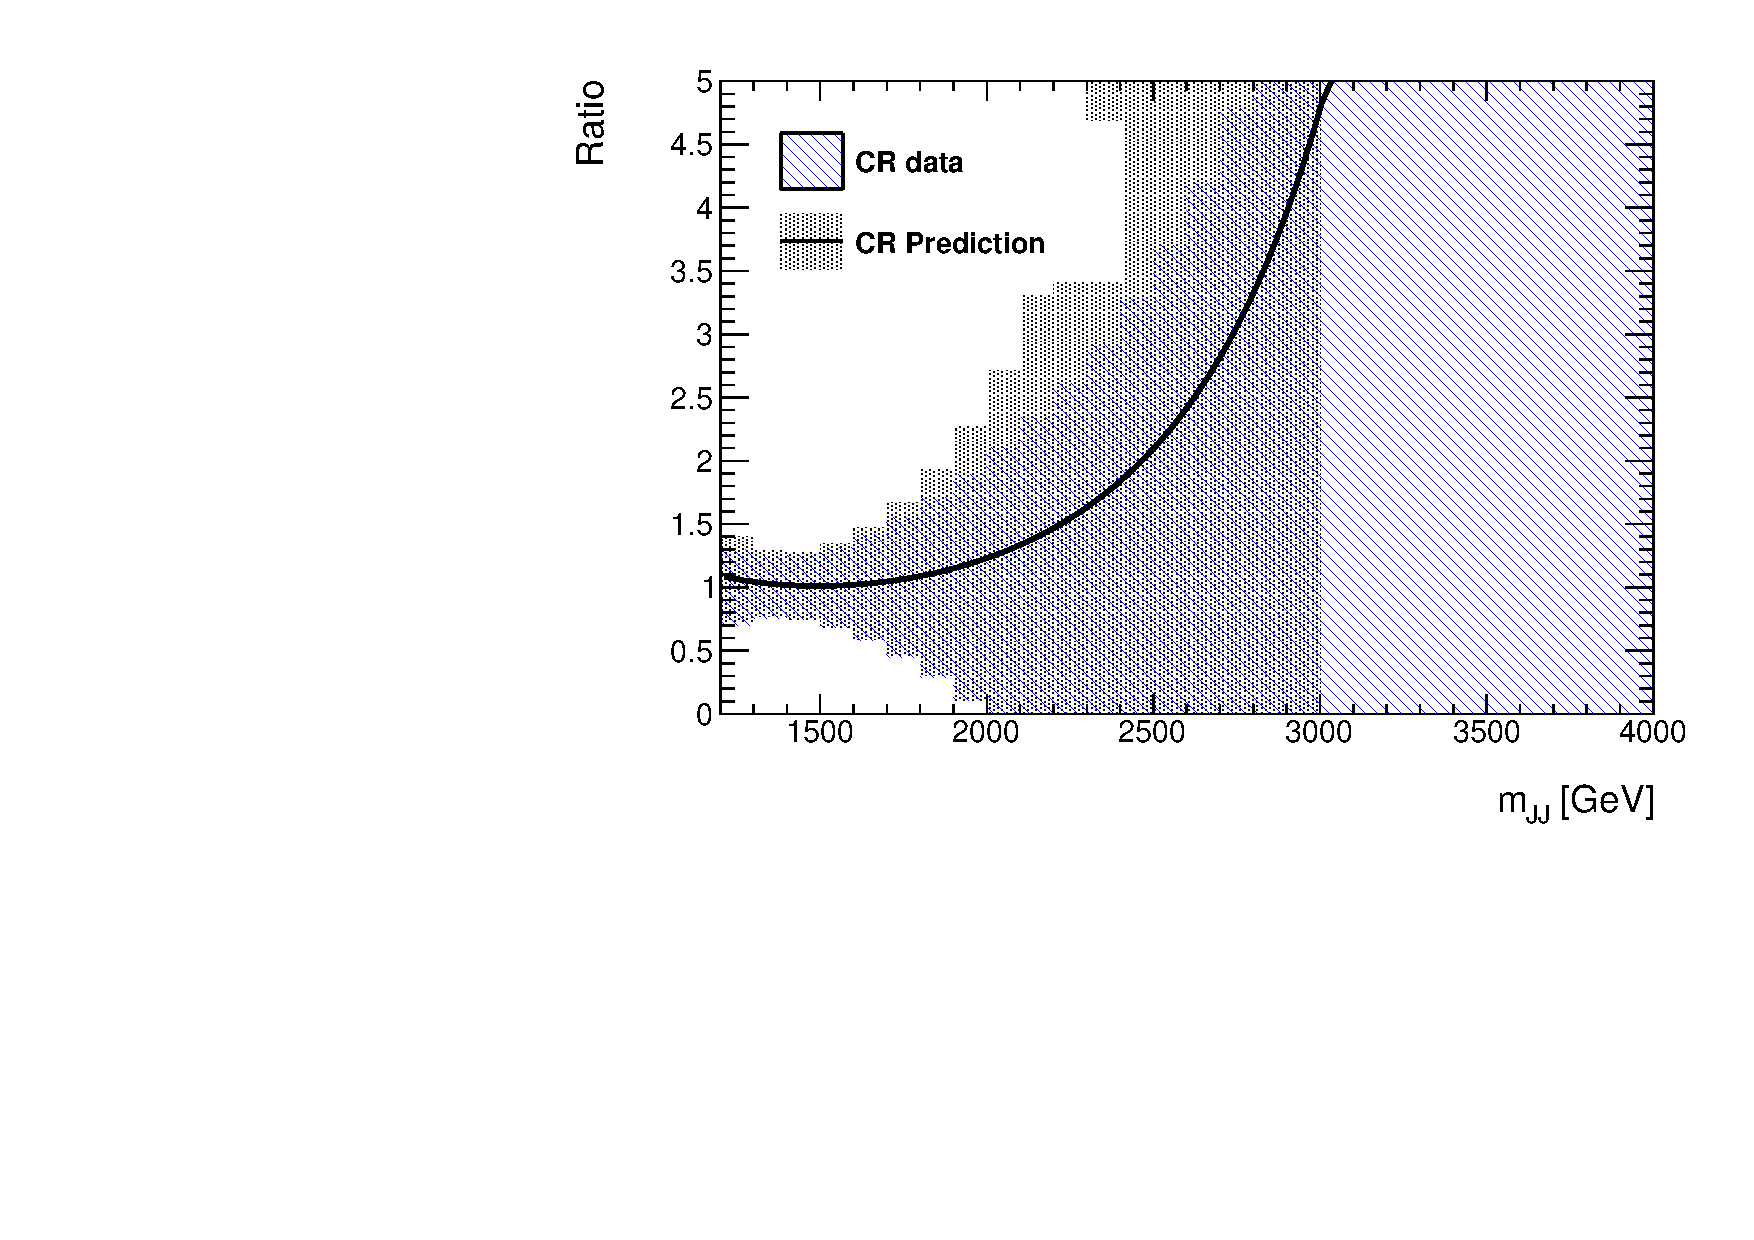
\includegraphics[width=0.4\textwidth,angle=-90]{figures/boosted/Syst_Shape/QCDSysfitSmooth_ratio_44.pdf} \\
\caption{Dijet mass distribution in the CR along with the prediction (left) and the ratio of the prediction to the CR distribution (right)  for the $2bs$ (top) $3b$ (middle) and $4b$ (bottom) samples.  Ratios are from the smoothed distributions, the data uncertainty band contains the smoothing parameter variations, and the prediction uncertainty band also contains smoothing parameter variations.}
\label{fig:qcd_shape_fit}
\end{center}
\end{figure}

%\begin{figure}[htbp!]
%\begin{center}
%%%\includegraphics[width=0.48\textwidth,angle=-90]{figures/boosted/systematics/QCDShapeSR/QCDShapeSR_44.pdf}
%%  %\includegraphics[width=0.48\textwidth,angle=-90]{figures/boosted/systematics/QCDShapeSR/QCDShapeSR_43.pdf}
%\caption{Effect of the up/down variation of the 2b QCD shape in the $4b$ (left) and $3b$ (right) signal regions. Gray lines show the upwards and downwards variations.  \textbf{TO BE UPDATED} }
%\label{fig:qcd_shape_signal}
%\end{center}
%\end{figure}

%%\begin{figure}[ht!]
%%\begin{center}
%%  %%\includegraphics[width=0.40\textwidth]{\figdir/systematics/QCD_shape/QCD_shape_scaled_signal.pdf}
%%  %%\includegraphics[width=0.40\textwidth]{\figdir/systematics/QCD_shape/QCD_shape_scaled_signal_log.pdf}
%%\caption{Effect of the up/down variation of the 2b+3b QCD shape in the signal region with a linear y-axis scale (left) and a log scale (right).}
%%\label{fig:qcd_shape_control}
%%\end{center}
%%\end{figure}

\clearpage
\subsubsection{Uncertainty on QCD smoothing function in the signal region}
\label{unc-smooth-qcd-in-sr}

%%\paragraph{}
The MJ8 function has been used to fit the QCD background prediction in order to smooth the distribution and provide non-zero background estimates up to dijet masses beyond which we have $1/2b$ statistics.  While this distribution is  observed to fit the $1/2b$ data well, it does not have a concrete physical motivation, and in principle the high mass tail of the distribution could be larger than predicted by an exponential.  Two checks are performed, changing the boundaries where the fit is performed, and changing the fit function.

%%\paragraph{}
To test the impact of the region in which the fit is performed, we varied the upper bound on the dijet fit region to be each of the values $\{2800,\ 3000,\ 3200\}$ GeV and the starting value between $\{1200,\ 1300,\ 1400\}$ GeV.  The ratio of the fits for each upper bound, to that of the nominal (1200-3000 GeV) can be found in Figure~\ref{fig:qcd_fit_range_sys_ratio-scaled}, along with a hash band showing the statistical uncertainty of the nominal fit.  The maximum deviation from the nominal fit, per bin, is taken as the shape systematic uncertainy.  This is estimated separately for $2bs$, $3b$, and $4b$ samples.

%%\paragraph{}
It should be noted that fits in which the fit $\chi^2$ probability was less than 0.001\%, or in which the fit integrals between 1500-2000 GeV, 2000-2500 GeV, or $>$2500 GeV were not in agreement with the original $1/2b$ distribution within a factor of 2 or 0.5, were not used to estimate the uncertainty.  The aforementioned checks ensure that we do not use poor fits of the $1/2b$ distribution to estimate the uncertainty.

%As we can see, changing the fit upper bound does not change the high mass tail prediction by large amounts, and is well within the statistical uncertainty of the nominal fit.  As a result, no additional systematic uncertainty is assigned for this fit range variation.

%\begin{figure}[htbp!]
%\begin{center}
%%%\includegraphics[width=0.48\textwidth,angle=-90]{figures/boosted/systematics/QCDFitFunc/QCDFitFuncSys_range_ratio_44.pdf}
%% %\includegraphics[width=0.48\textwidth,angle=-90]{figures/boosted/systematics/QCDFitFunc/QCDFitFuncSys_range_ratio_43.pdf}
%\caption{The ratio of the nominal exponential QCD prediction of the dijet mass distribution(with hashed band statistical uncertainties) to the predictions when fit with different upper bounds, in the $4b$ (left) and $3b$ (right) signal regions.  \textbf{TO BE UPDATED} }
%\label{fig:qcd_fit_range_sys_ratio}
%\end{center}
%\end{figure}

%The same test of changing the fit range for the scaled dijet mass distribution in the $4b$ and $3b$ signal regions has been performed, and the ratio of the different fit functions can be found in Figure~\ref{fig:qcd_fit_range_sys_ratio-scaled}.

\begin{figure}[htbp!]
\begin{center}
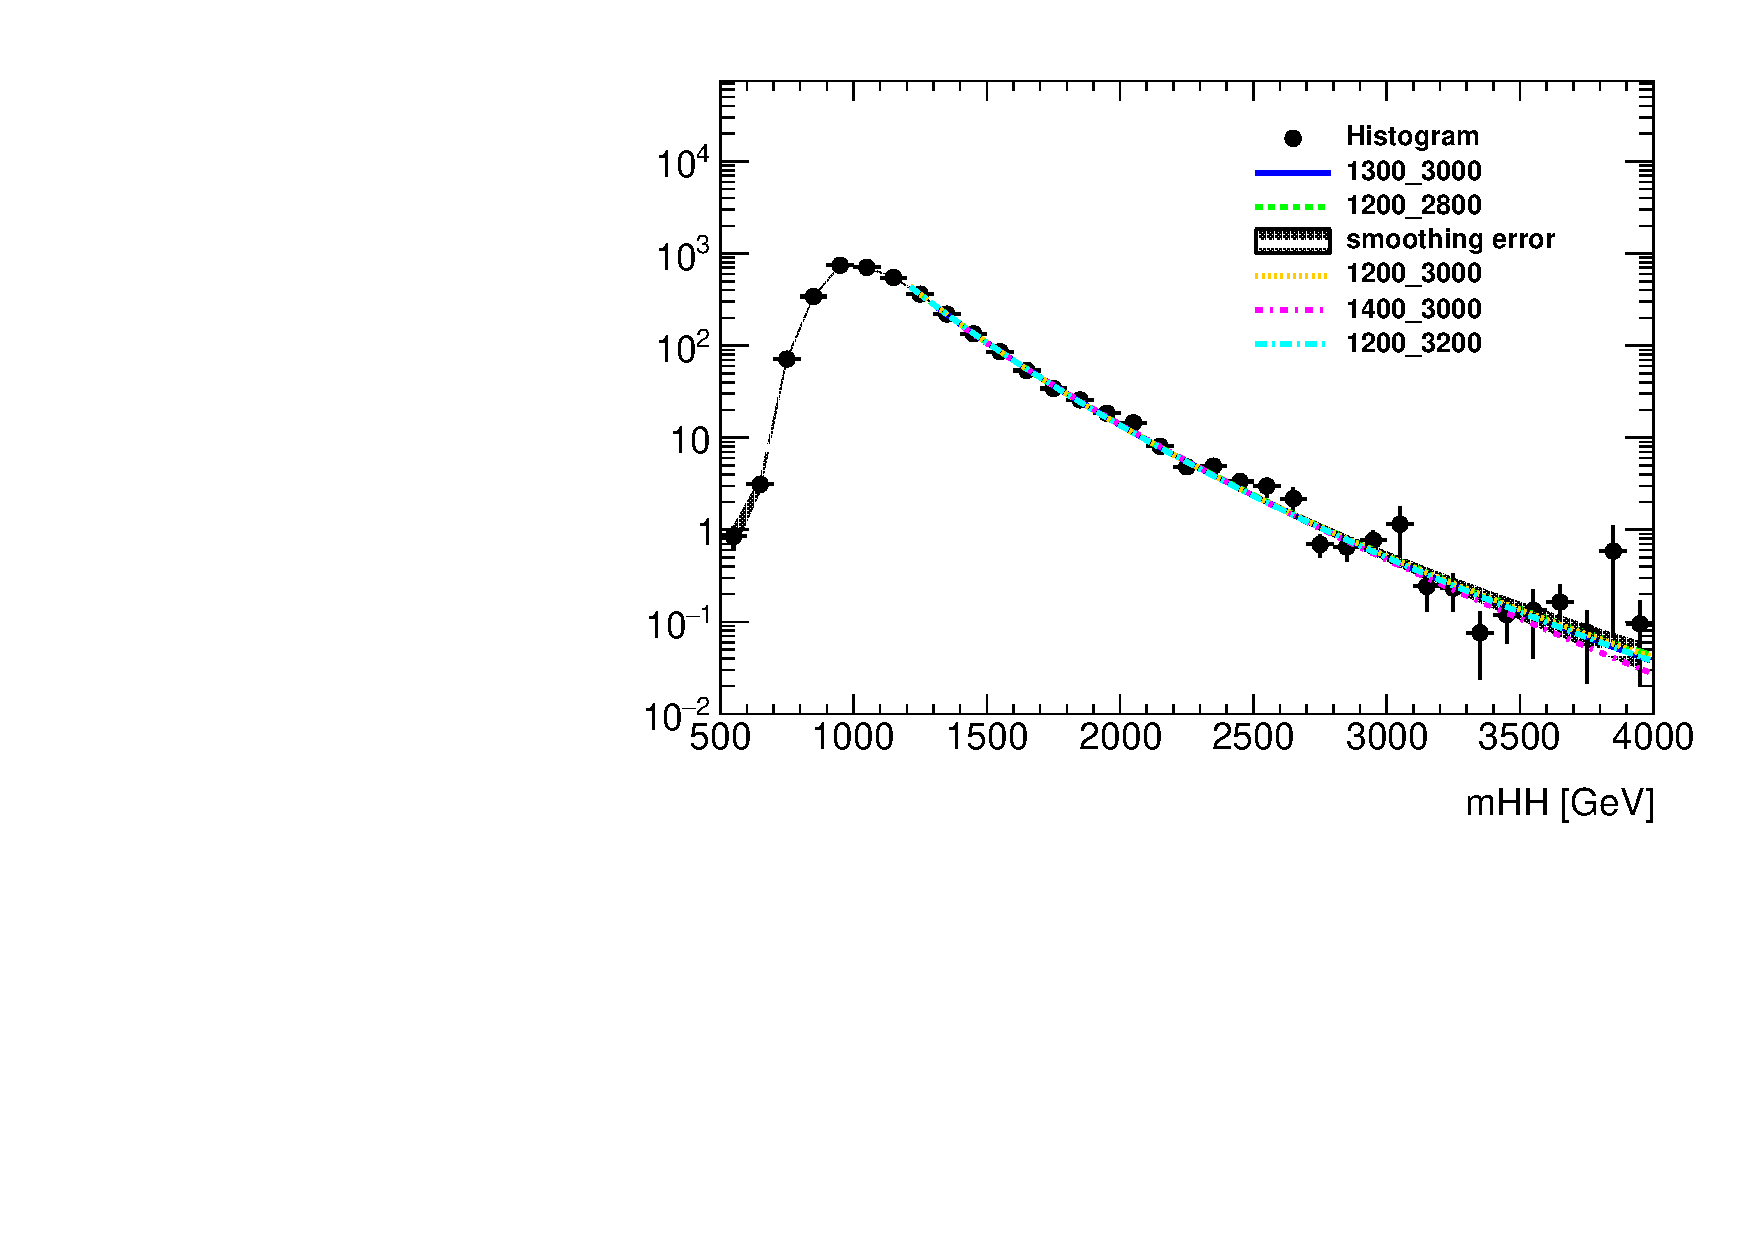
\includegraphics[width=0.48\textwidth,angle=-90]{figures/boosted/Syst_Smooth/smoothFuncRangeCompare_22_comp.pdf}
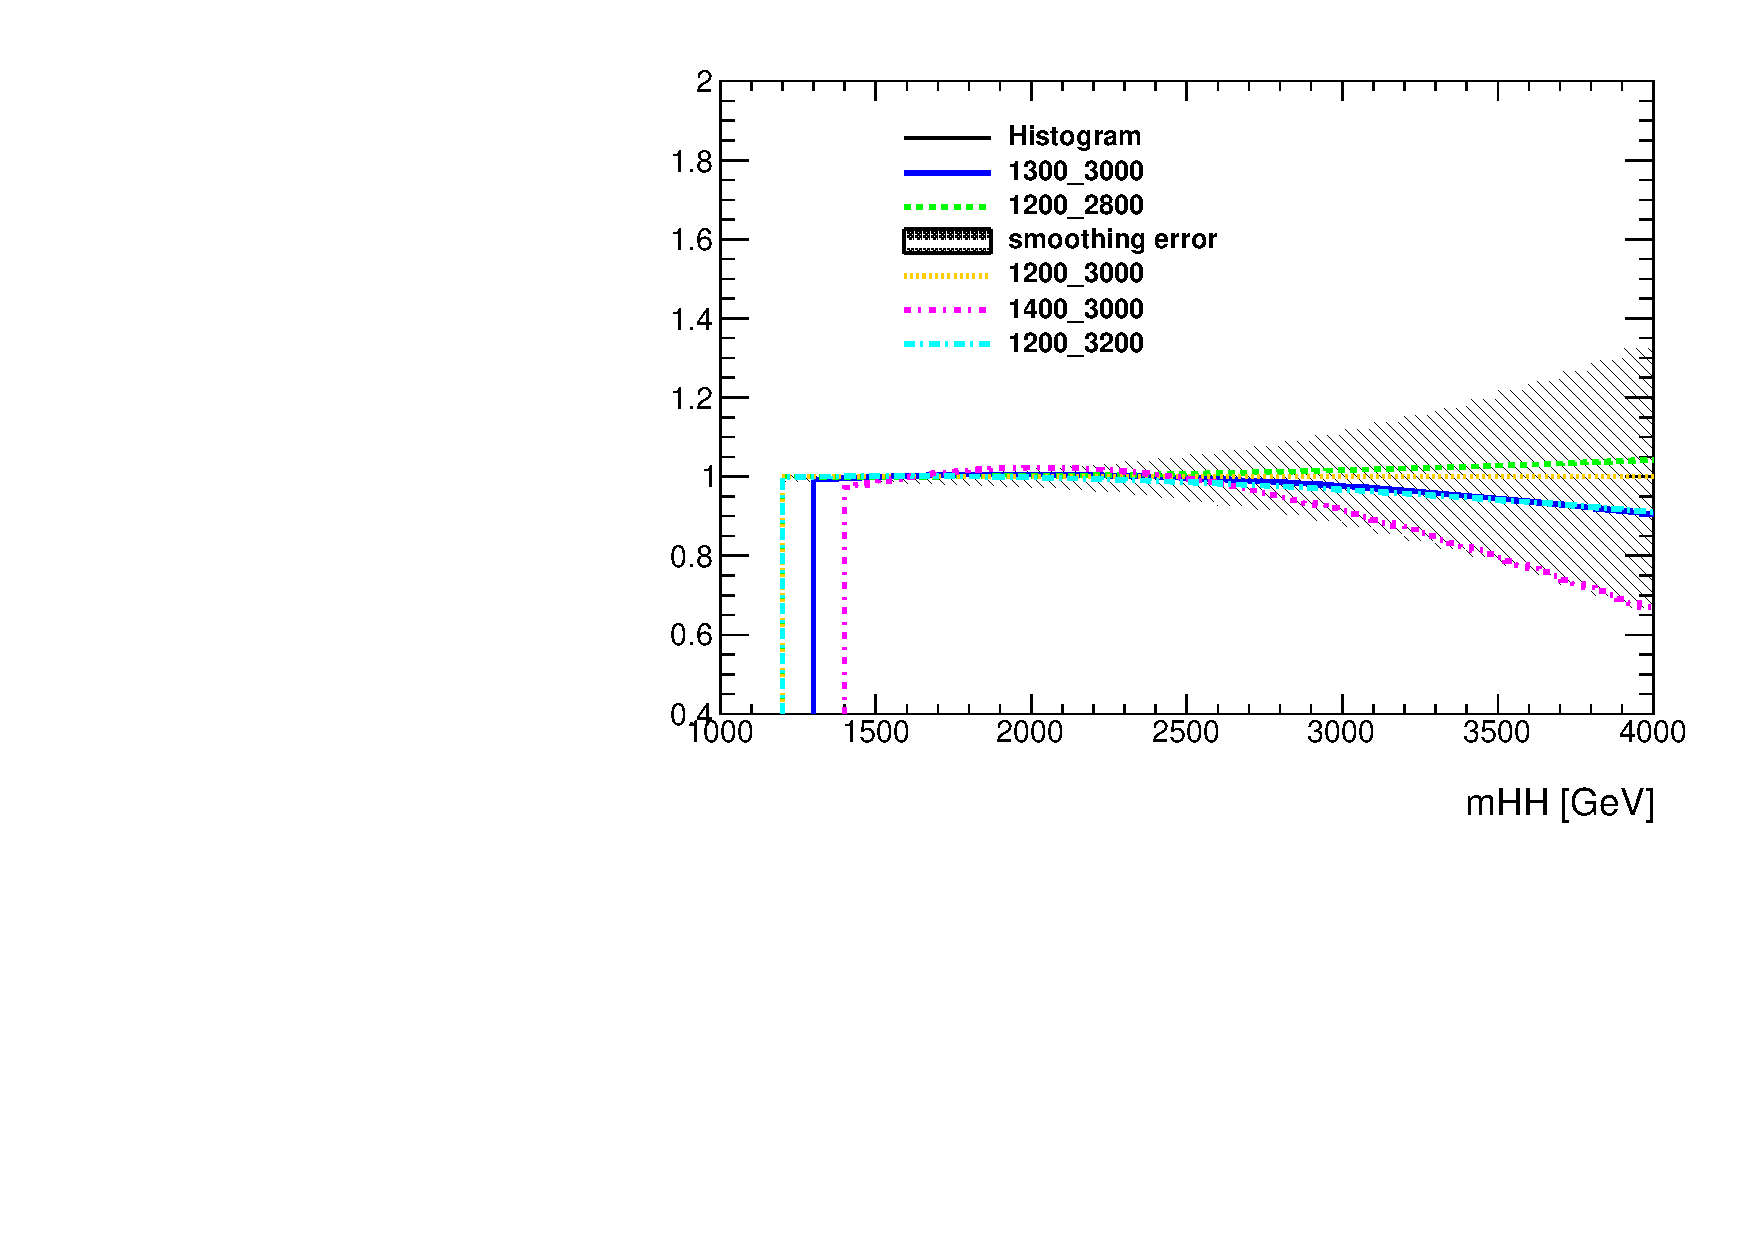
\includegraphics[width=0.48\textwidth,angle=-90]{figures/boosted/Syst_Smooth/smoothFuncRangeCompare_22_comp_ratio.pdf} \\
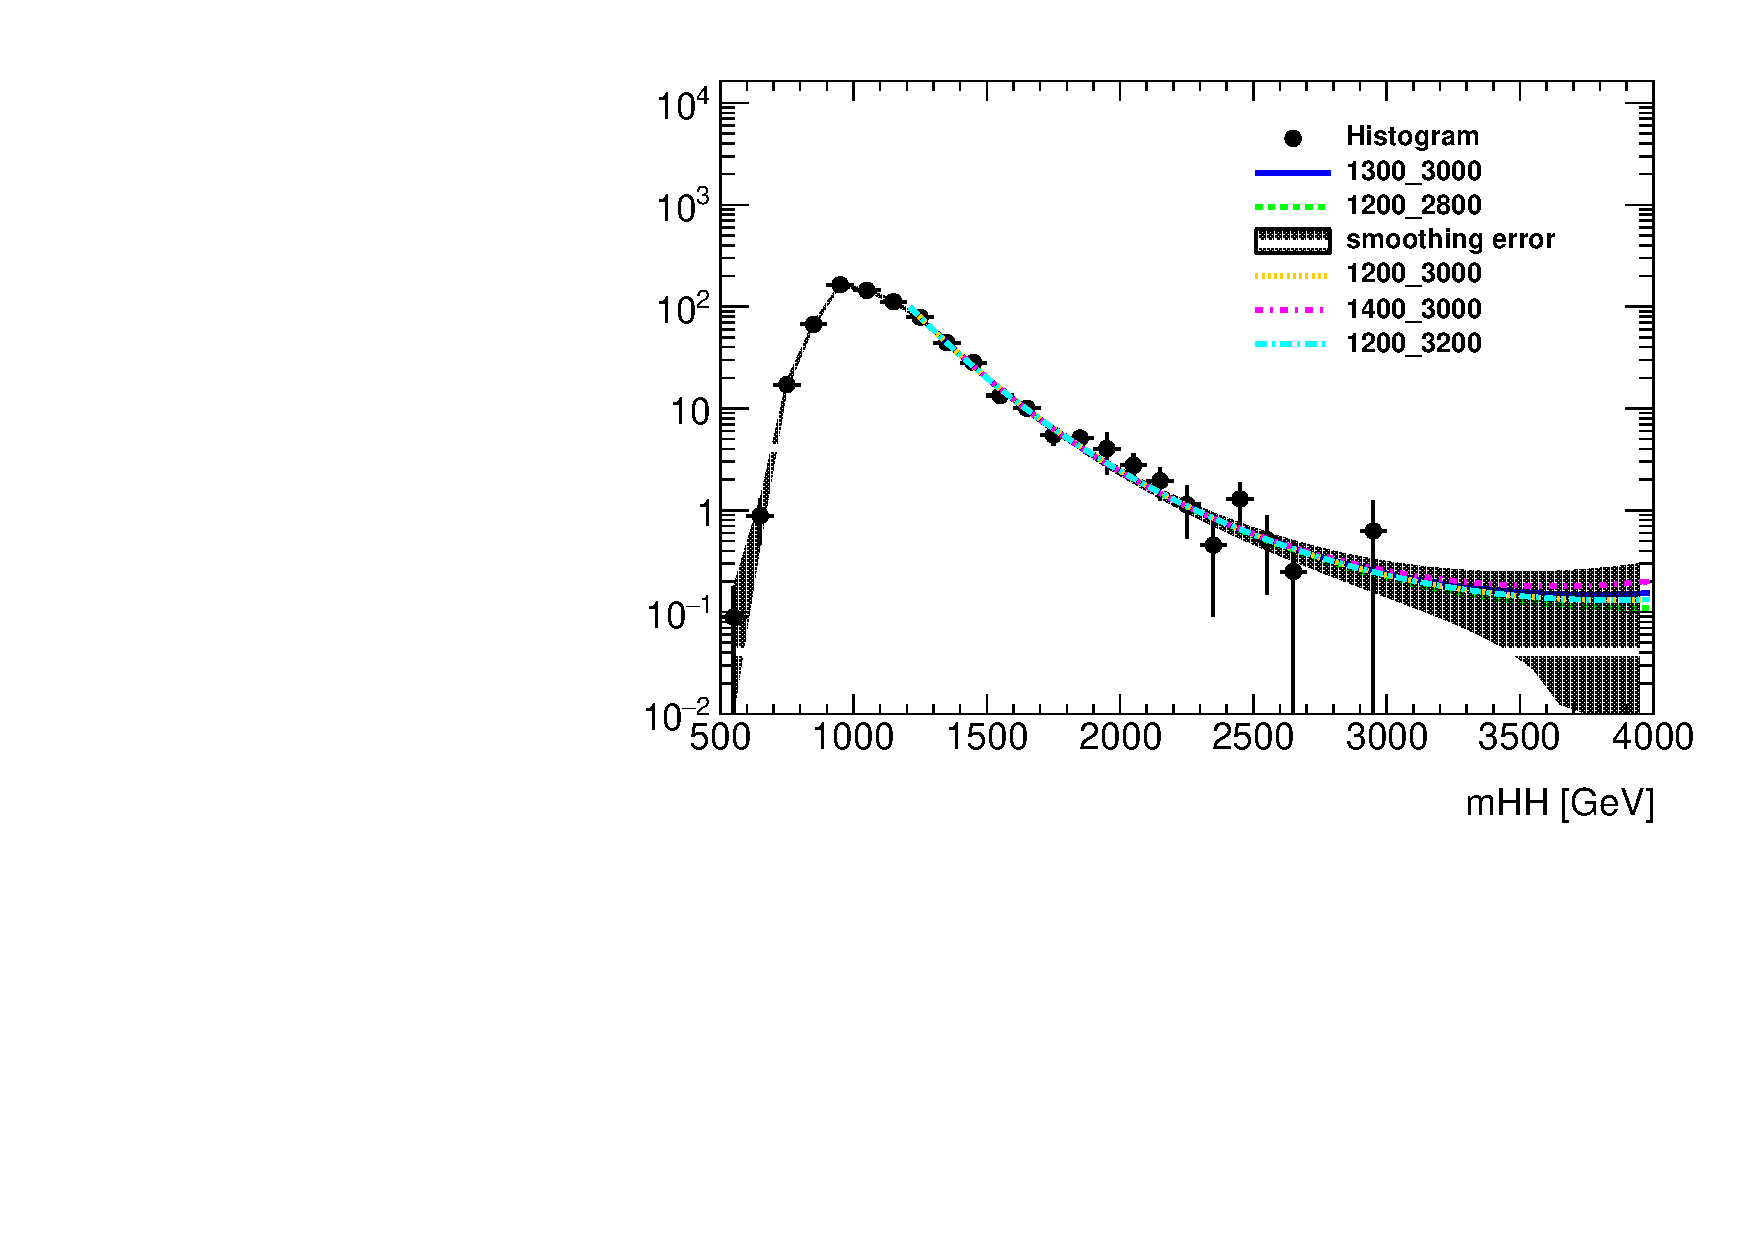
\includegraphics[width=0.48\textwidth,angle=-90]{figures/boosted/Syst_Smooth/smoothFuncRangeCompare_33_comp.pdf}
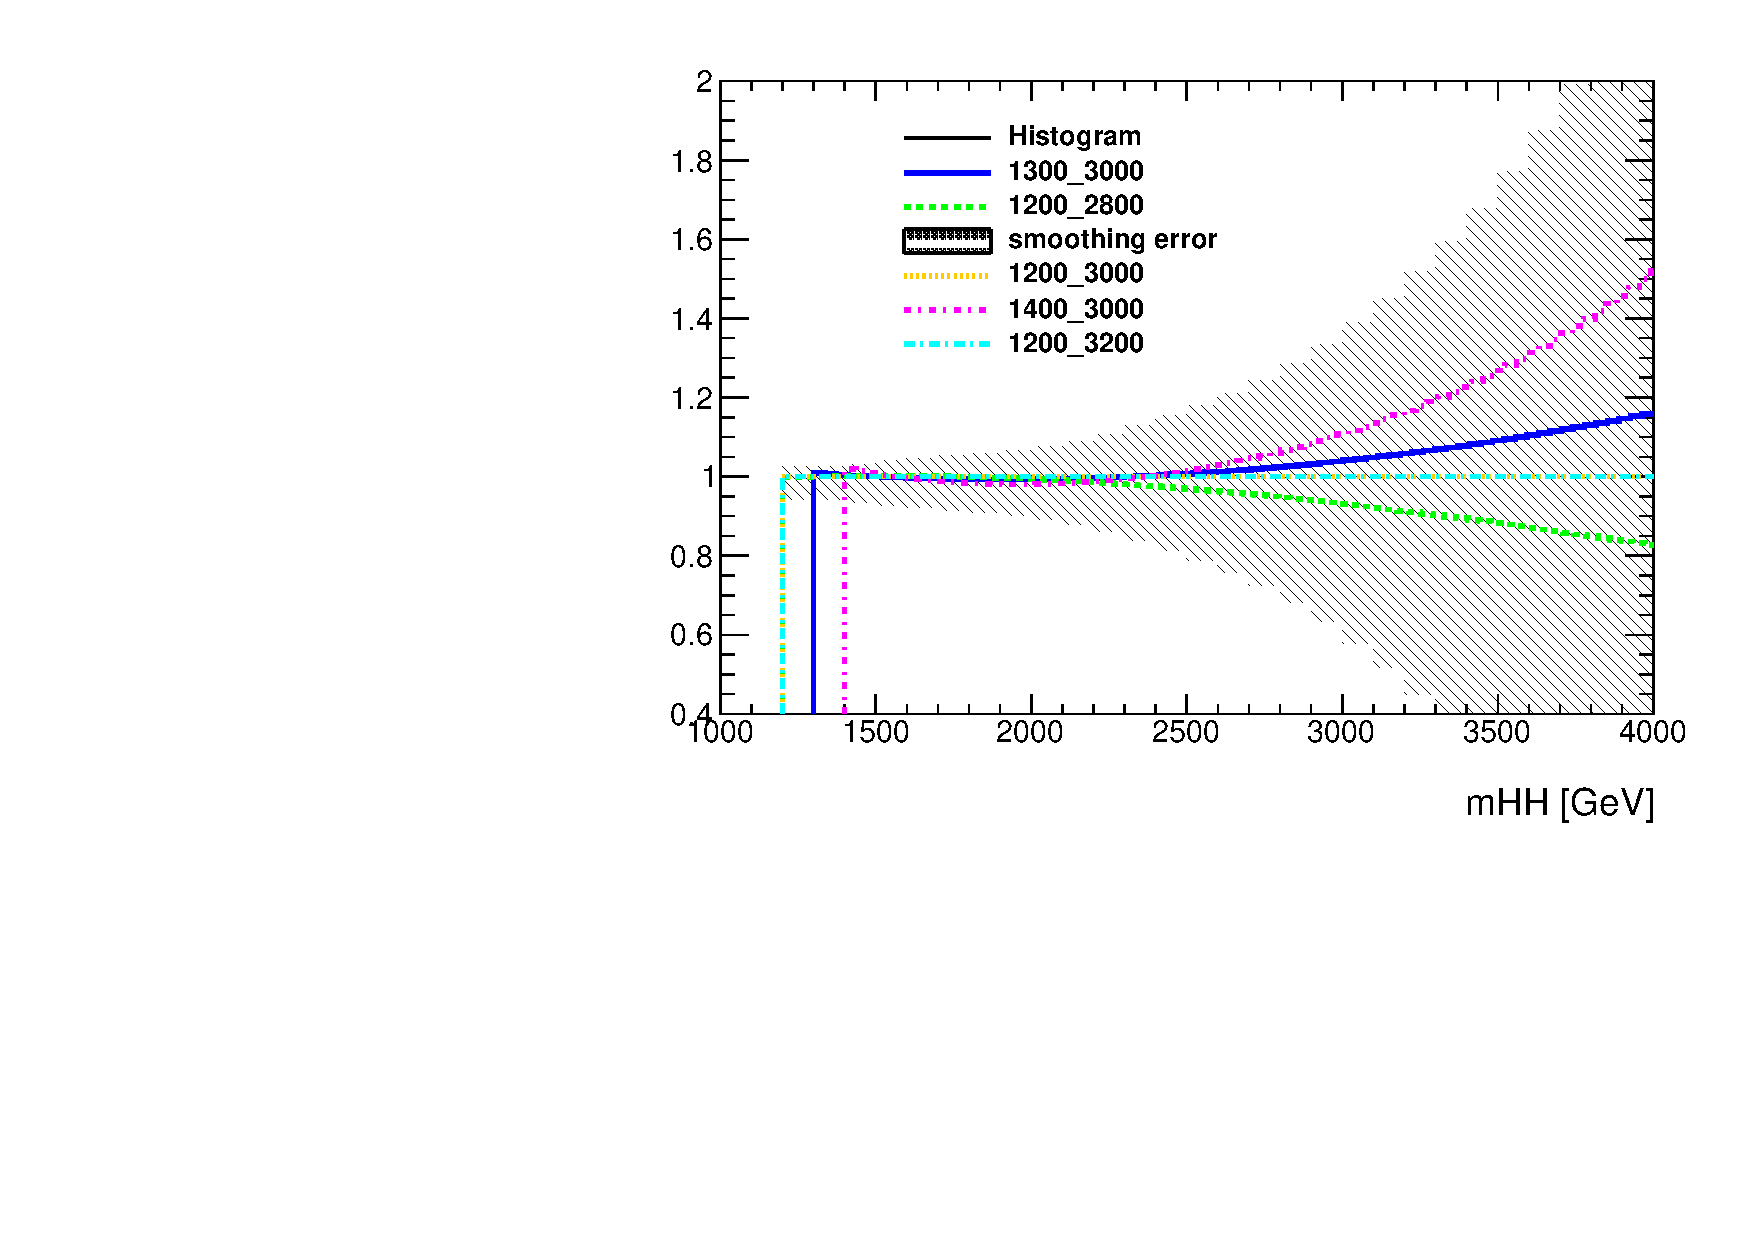
\includegraphics[width=0.48\textwidth,angle=-90]{figures/boosted/Syst_Smooth/smoothFuncRangeCompare_33_comp_ratio.pdf} \\
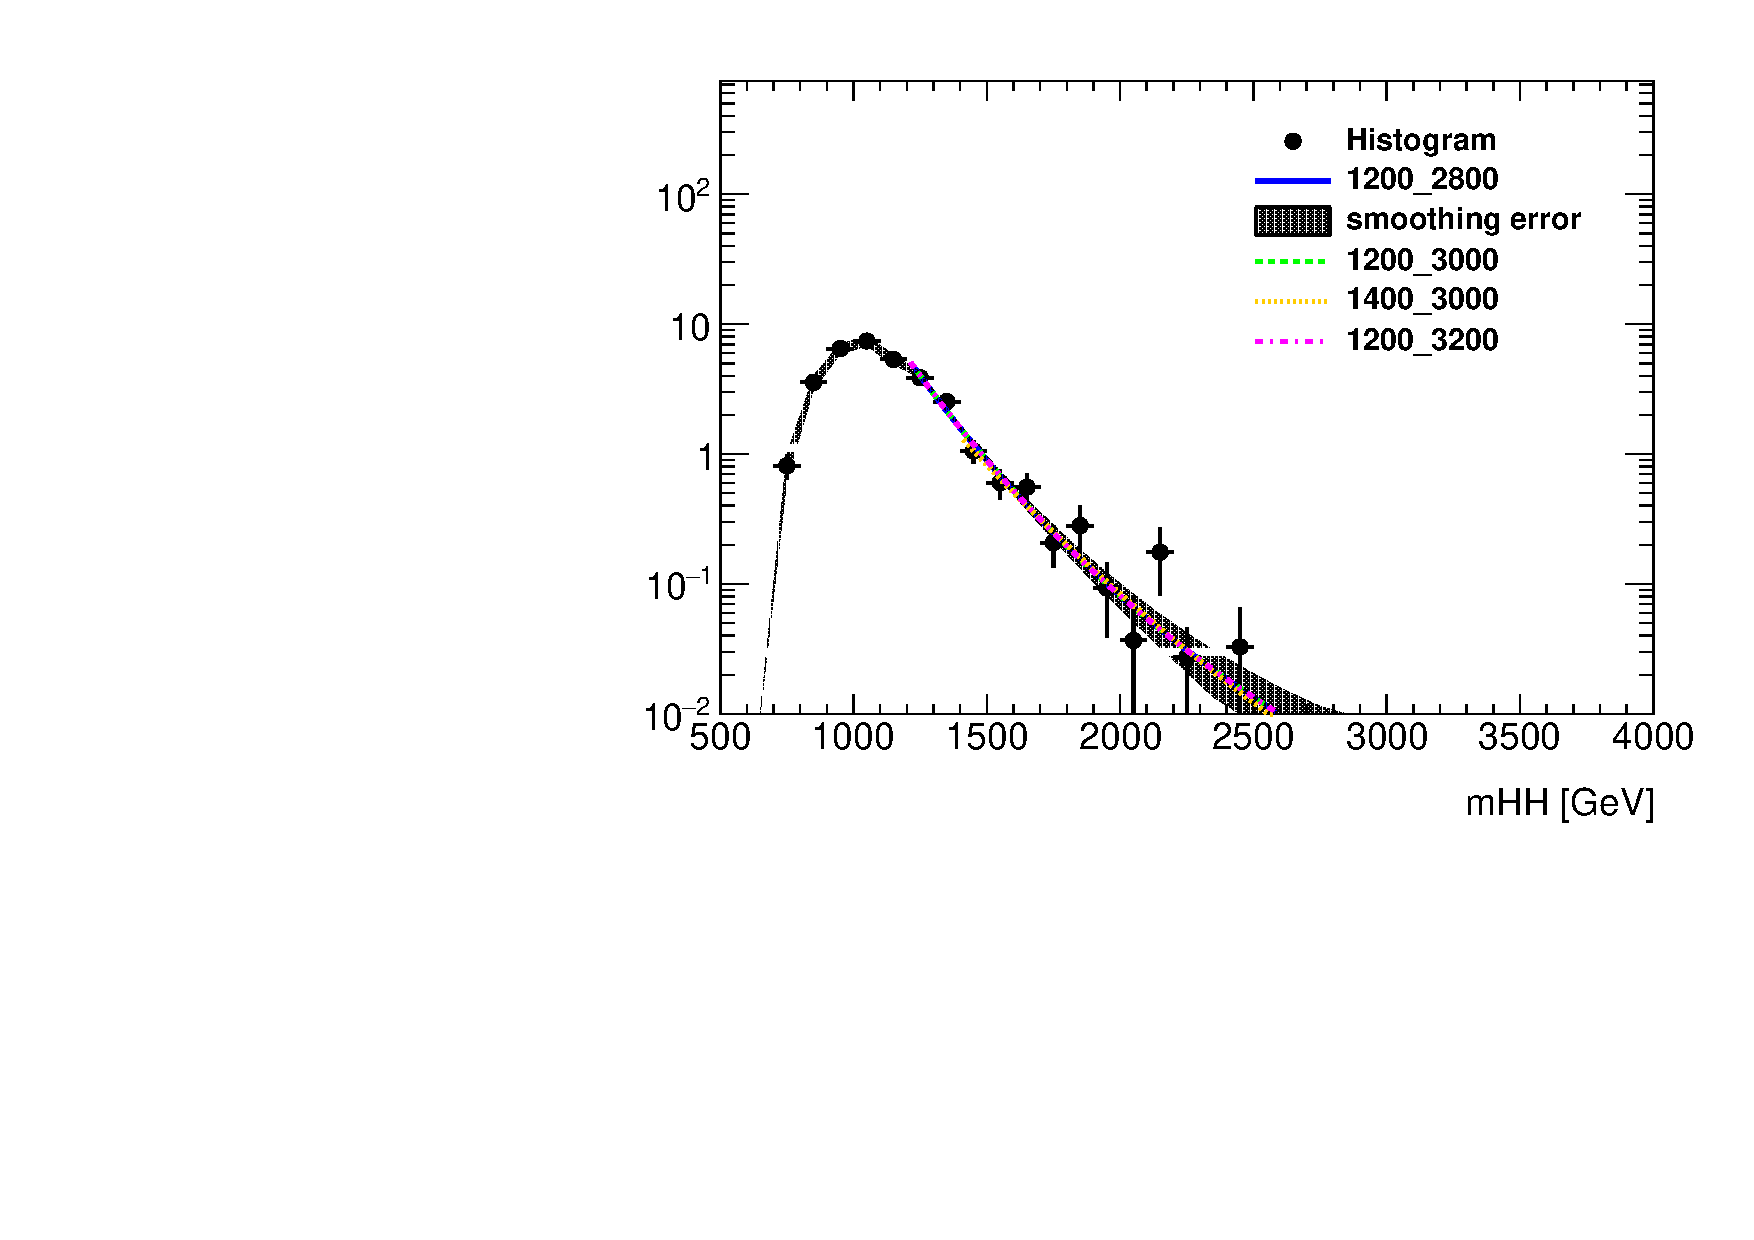
\includegraphics[width=0.48\textwidth,angle=-90]{figures/boosted/Syst_Smooth/smoothFuncRangeCompare_44_comp.pdf}
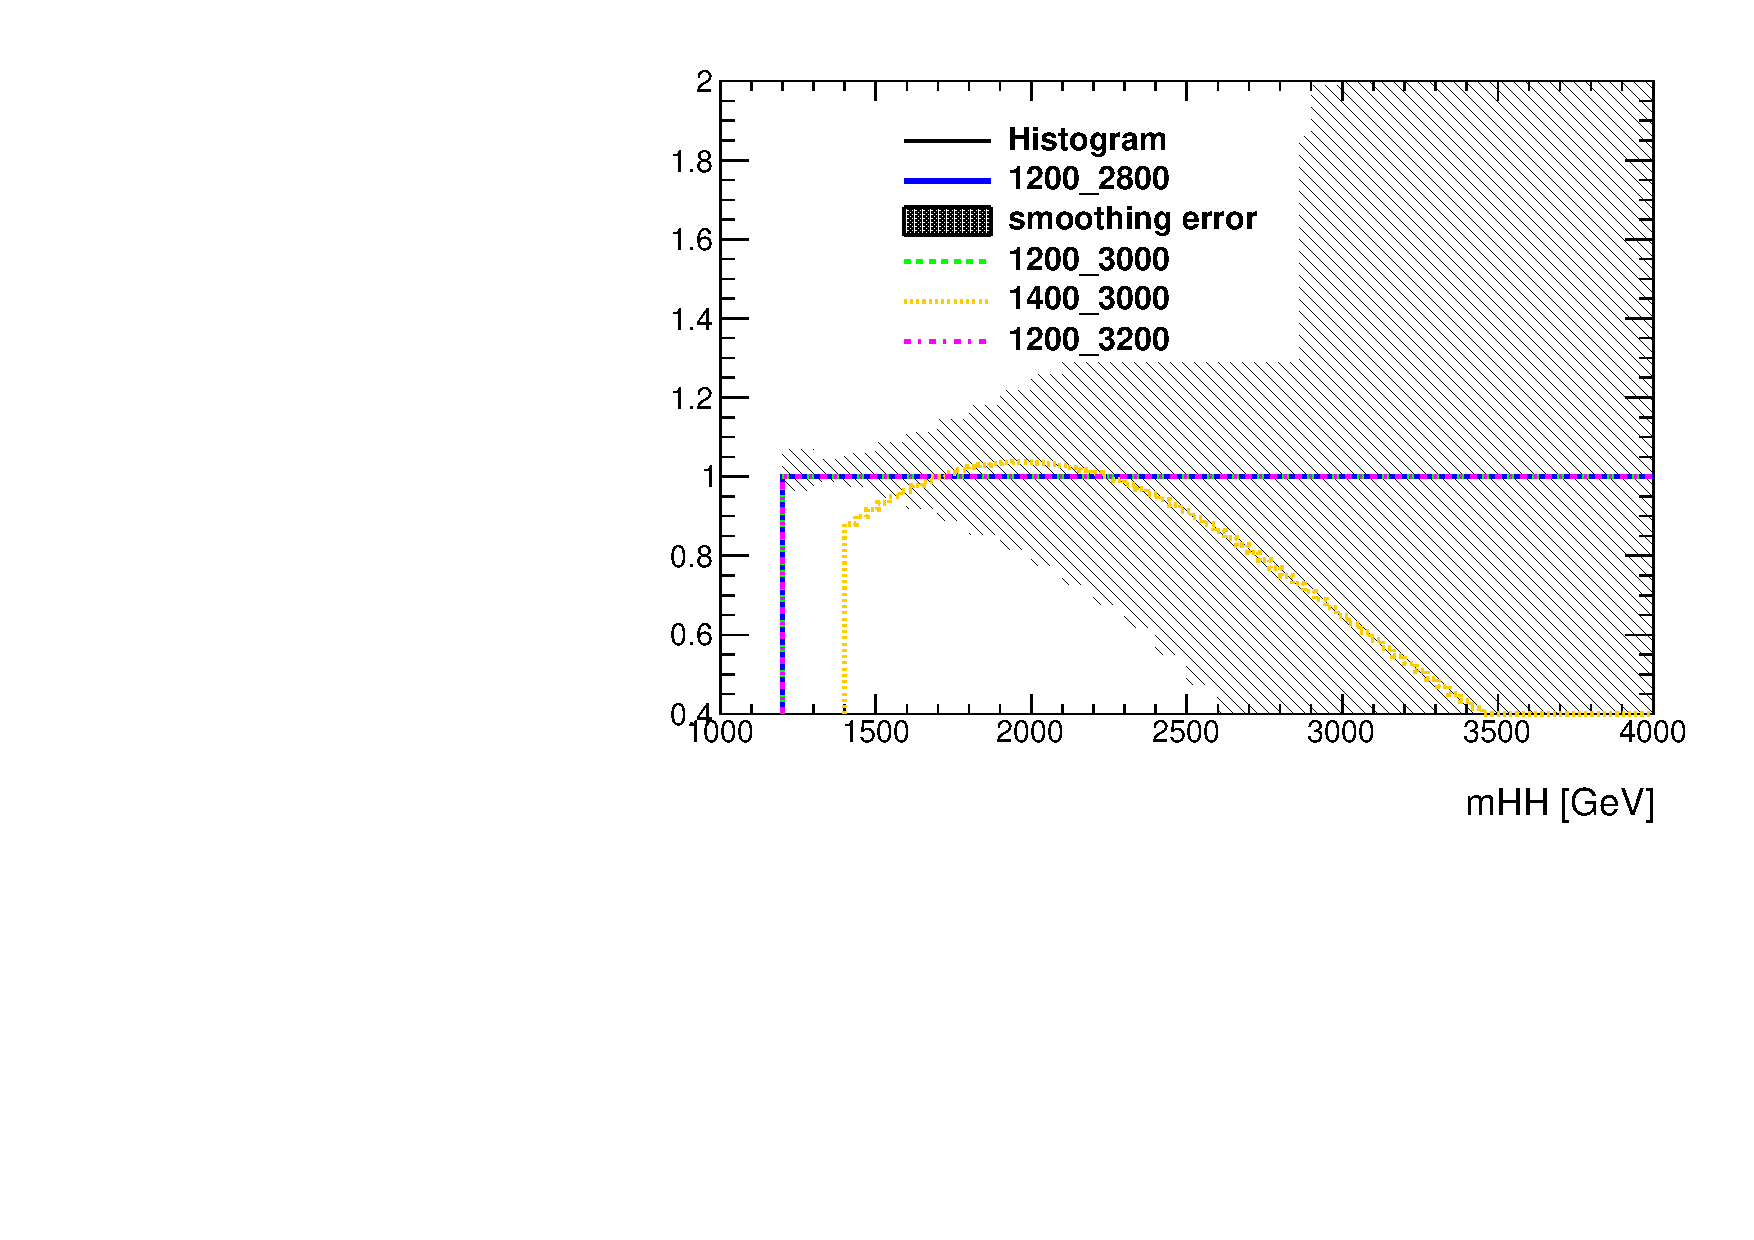
\includegraphics[width=0.48\textwidth,angle=-90]{figures/boosted/Syst_Smooth/smoothFuncRangeCompare_44_comp_ratio.pdf} \\
\caption{Dijet mass distribution SR prediction fit with several fit ranges (left) and the ratio of nominal to fits with different fit ranges (right)  for the 2b (top) 3b (middle) and 4b (bottom) samples. }
\label{fig:qcd_fit_range_sys_ratio-scaled}
\end{center}
\end{figure}

%%\paragraph{}
As a second test, we fit the $1/2b$ QCD prediction with a variety of other distributions which can show both power law behavior in the bulk of the distribution as well as longer tails.  The set of additional functions examined (labelled MJ1-MJ7) can be found in Table~\ref{tab:fit_funcs}, where $x = m_{JJ} / \sqrt{s}$.

\begin{table}[htbp!]
\begin{center} 
\begin{tabular}{  l | c}
%\footnotesize
Name & Functional Form \\
\hline
MJ1 (Dijet) & $f_{1}(x) = p_0 (1-x)^{p_1} x^{p_2}$ \\
MJ2 & $f_{2}(x) = p_0 (1-x)^{p_1} e^{p_2\ x^2}$ \\
MJ3 & $f_{3}(x) = p_0 (1-x)^{p_1} x^{p_2\ x}$ \\
MJ4 & $f_{4}(x) = p_0 (1-x)^{p_1} x^{p_2\ ln\ x}$ \\
MJ5 & $f_{5}(x) = p_0 (1-x)^{p_1} (1+x)^{p_2\ x}$ \\
MJ6 & $f_{6}(x) = p_0 (1-x)^{p_1} (1+x)^{p_2\ ln\ x}$ \\
MJ7 & $f_{7}(x) = \frac{p_0}{x} (1-x)^{p_1 - p_2\ ln\ x}$ \\
MJ8 & $f_{8}(x) = \frac{p_0}{x^2} (1-x)^{p_1 - p_2\ ln\ x}$ \\
\hline
\end{tabular}
\caption{Functions used to fit the QCD dijet mass distributions, where $x = m_{JJ} / \sqrt{s}$.}
\label{tab:fit_funcs}
\end{center}
\end{table}

%%\paragraph{}
Figure~\ref{fig:qcd_fit_funcs_sys} shows the fits to the QCD prediction in the 4/3/2b  signal regions, and the nominal dijet fit, as well as the ratios of the nominal fit to that of the additional functions.  The maximum per bin deviation is taken as the shape systematic, separately for the 4/3/2b SRs.

%%\paragraph{}
As before, fits in which the fit $\chi^2$ probability was less than 0.1\%,  or in which the fit integrals between 1500-2000 GeV, 2000-2500 GeV, or $>$2500 GeV were not in agreement with the original 0b distribution within a factor of 2 or 0.5, were not used to estimate the uncertainty.  The aforementioned checks ensure that we do not use poor fits of the 0b distribution to estimate the uncertainty.

\begin{figure}[htbp!]
\begin{center}
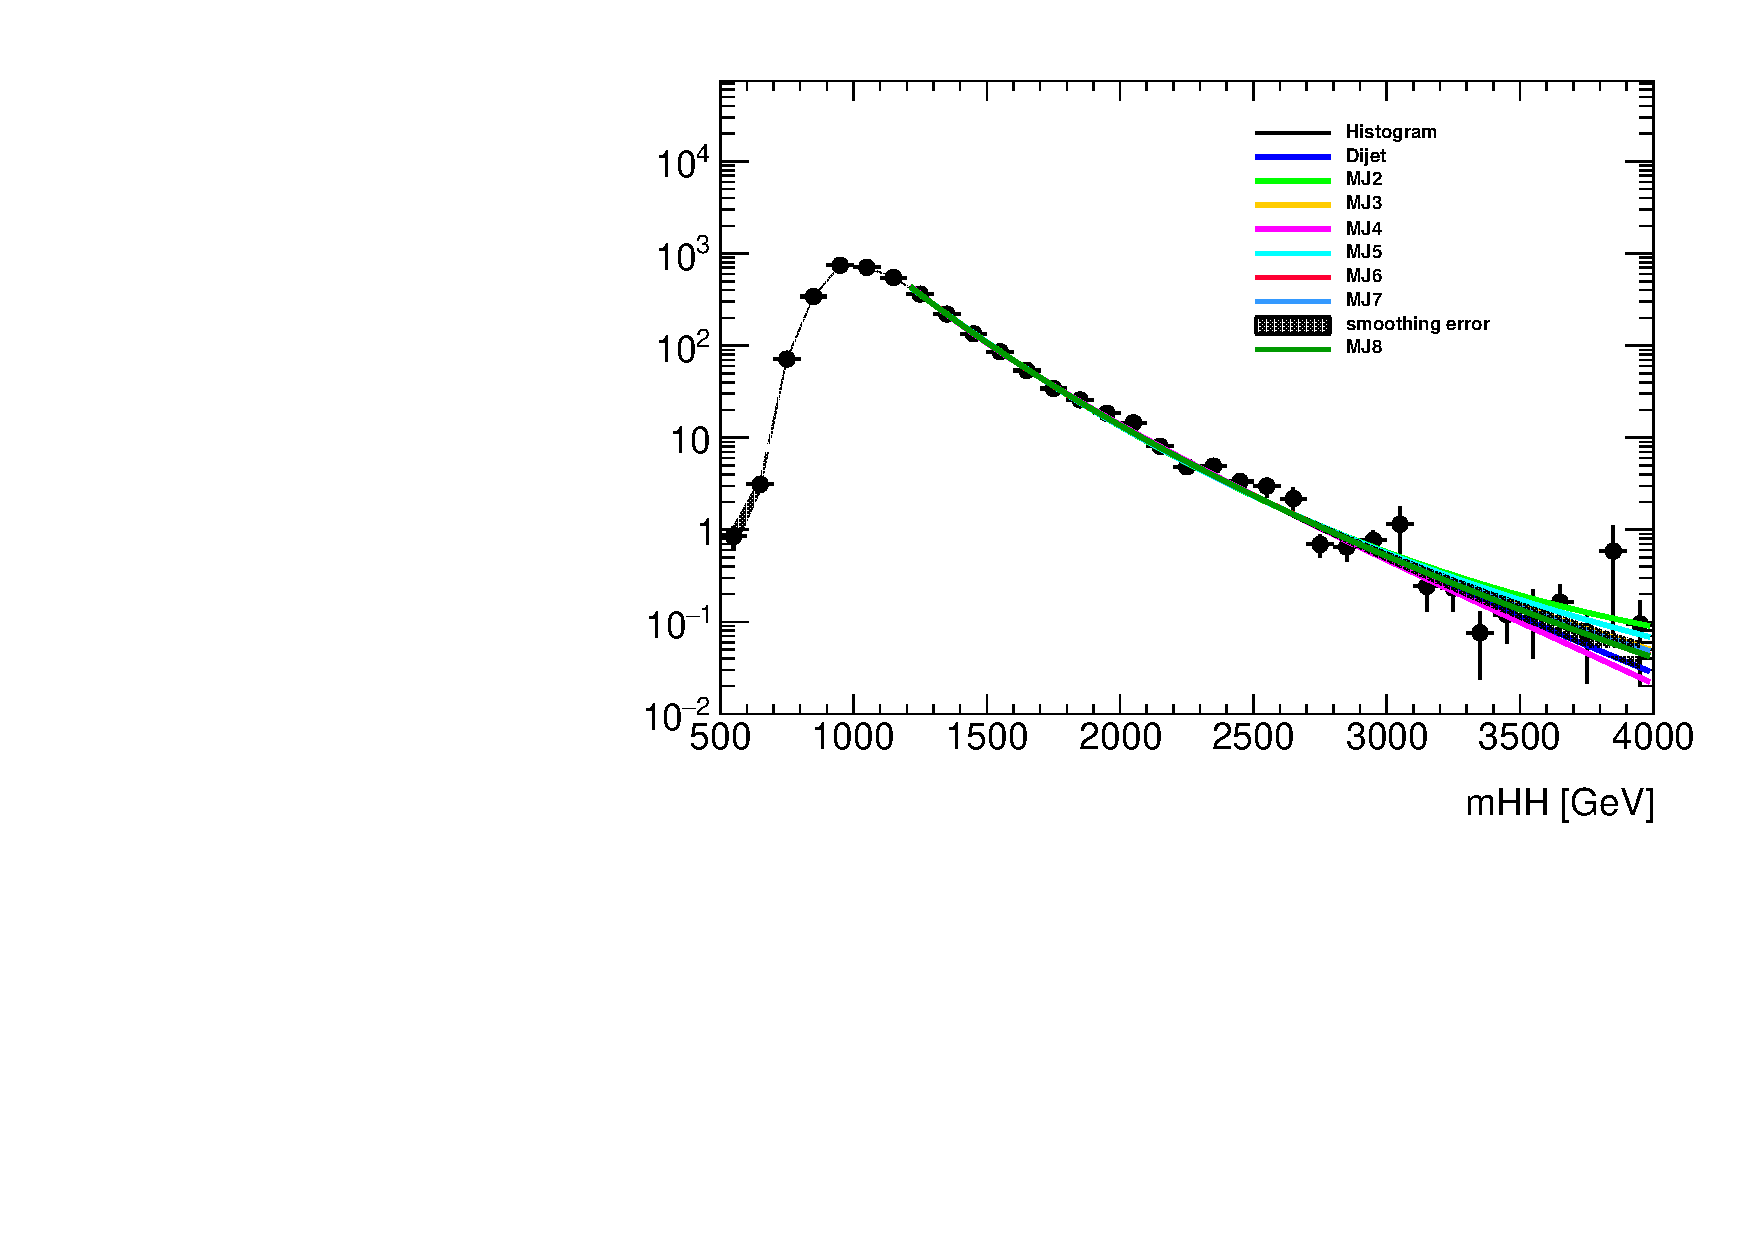
\includegraphics[width=0.48\textwidth,angle=-90]{figures/boosted/Syst_Smooth/smoothFuncCompare_22_comp.pdf}
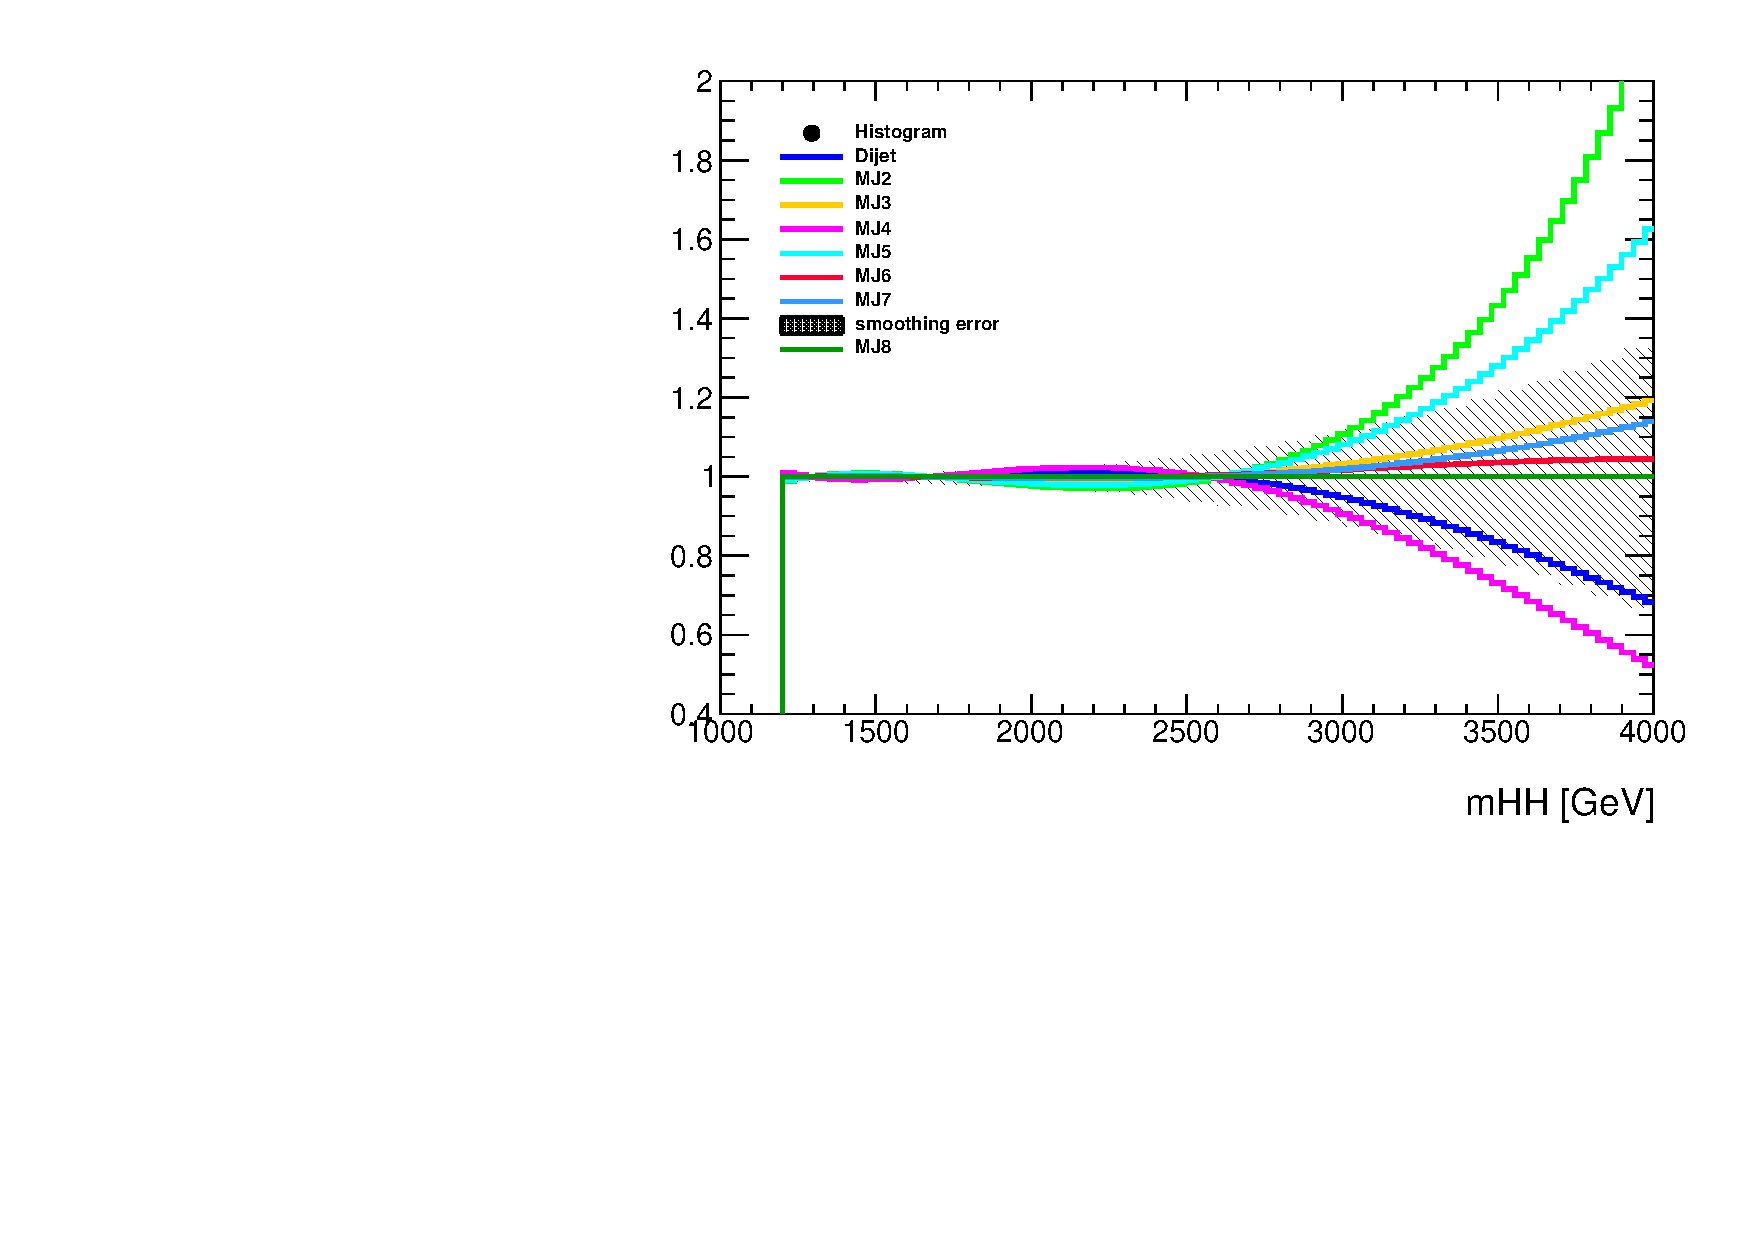
\includegraphics[width=0.48\textwidth,angle=-90]{figures/boosted/Syst_Smooth/smoothFuncCompare_22_comp_ratio.pdf} \\
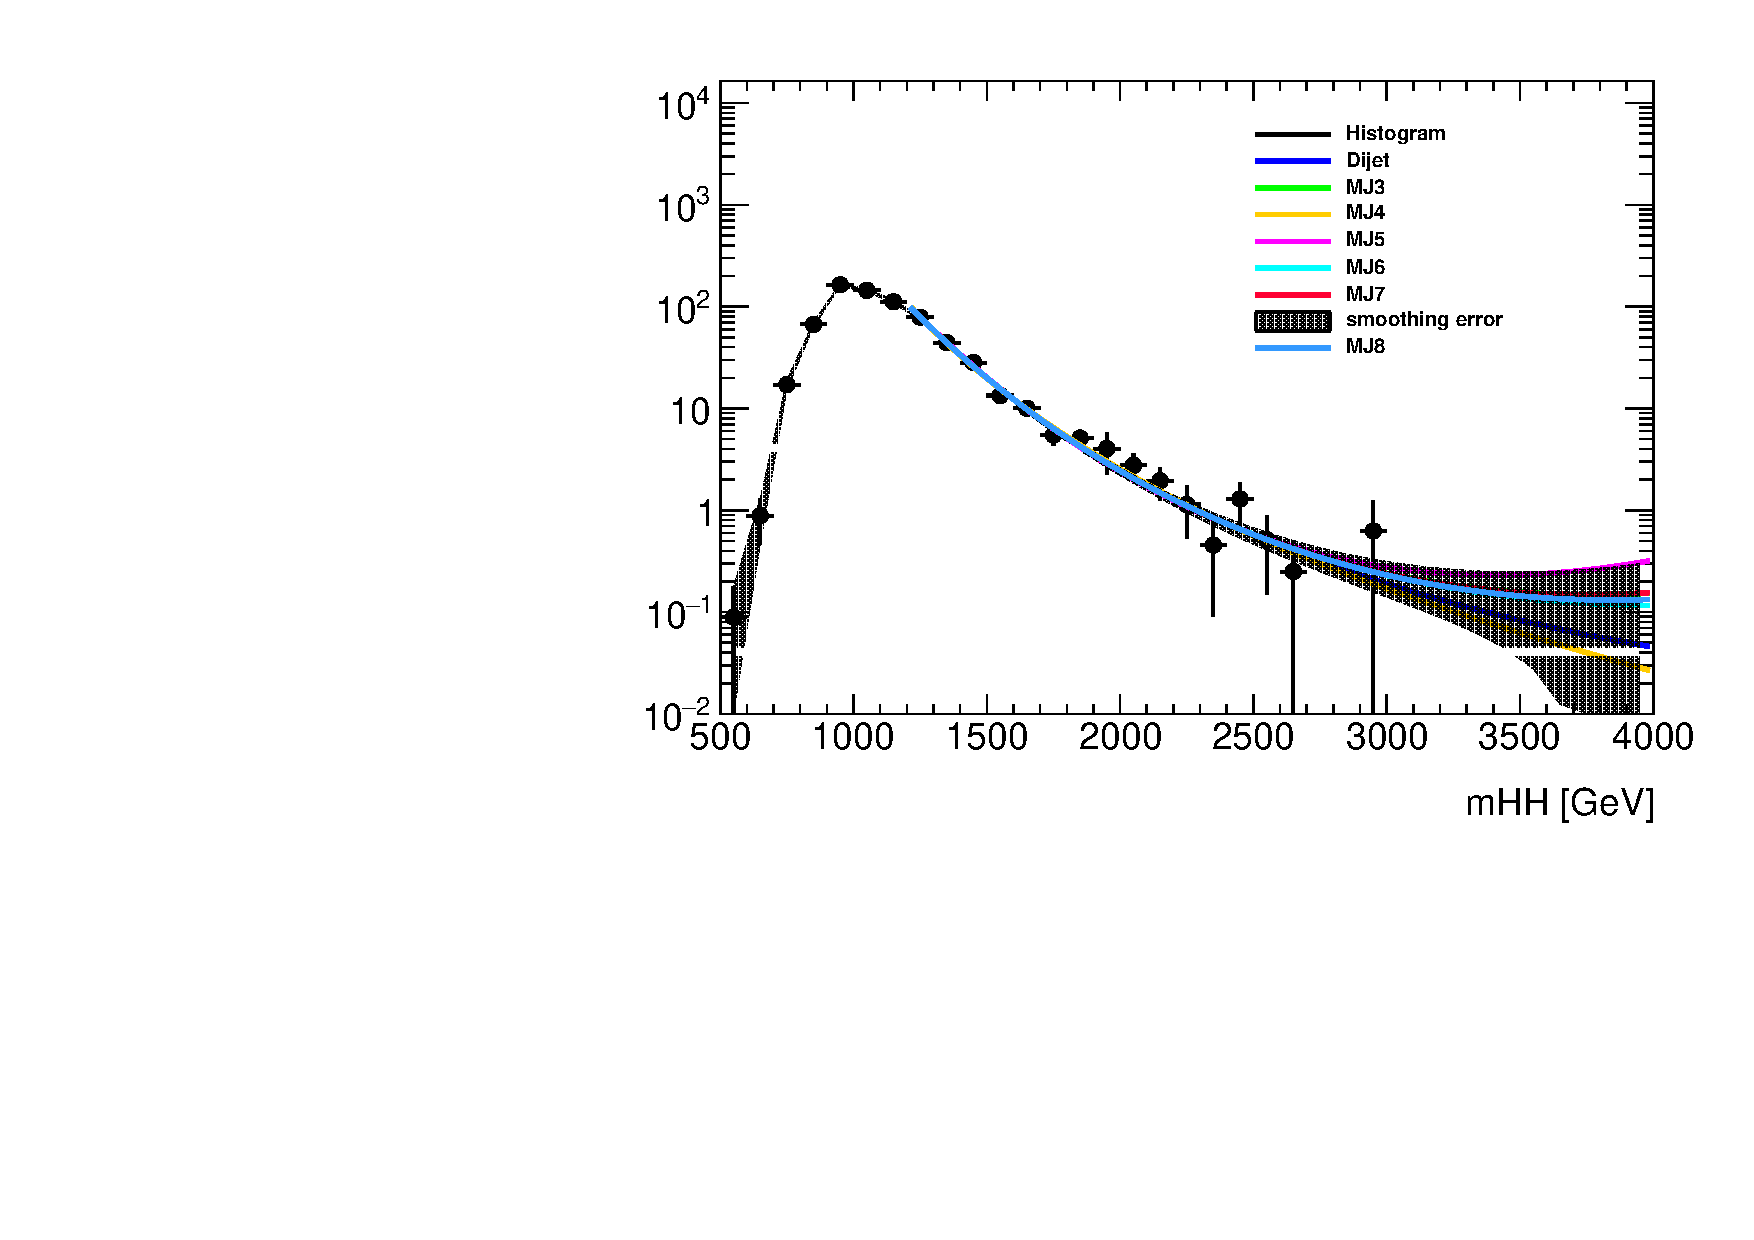
\includegraphics[width=0.48\textwidth,angle=-90]{figures/boosted/Syst_Smooth/smoothFuncCompare_33_comp.pdf}
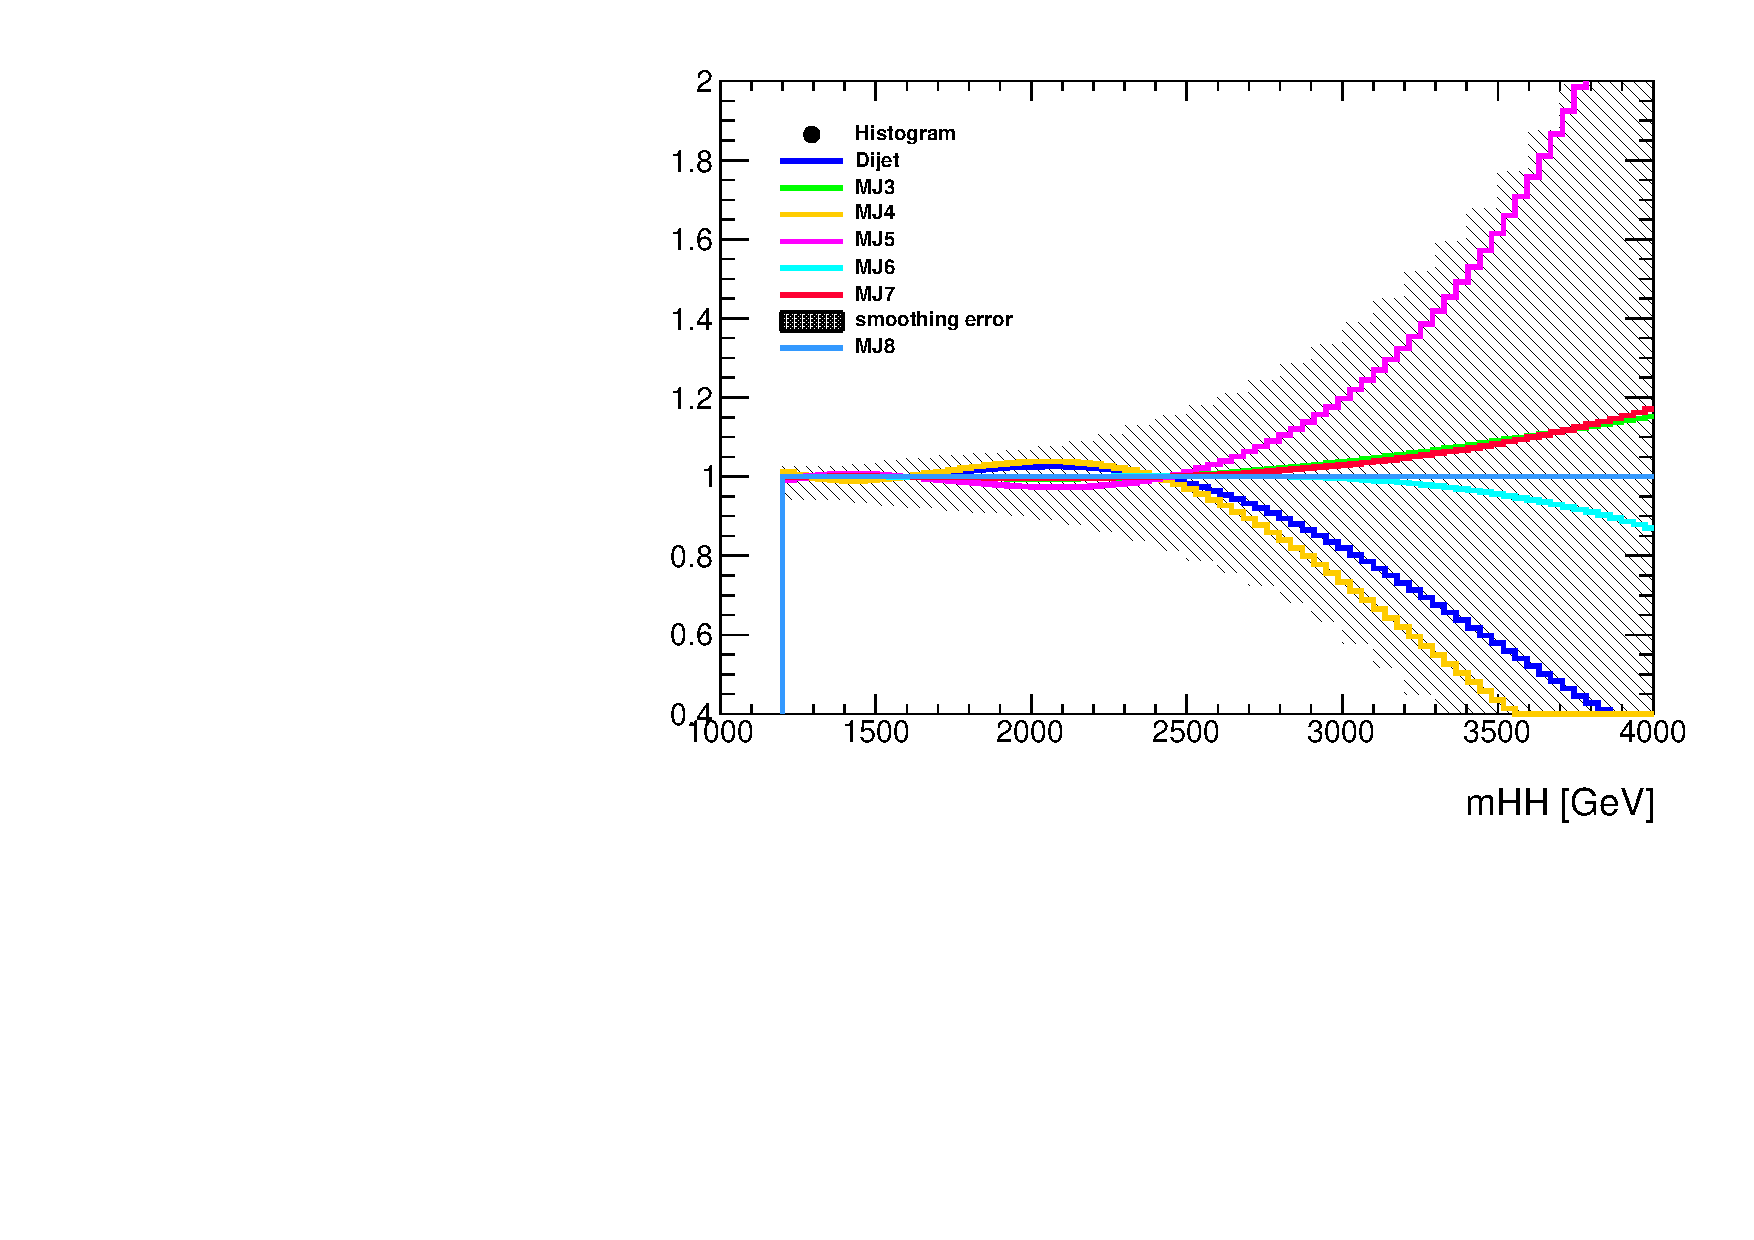
\includegraphics[width=0.48\textwidth,angle=-90]{figures/boosted/Syst_Smooth/smoothFuncCompare_33_comp_ratio.pdf} \\
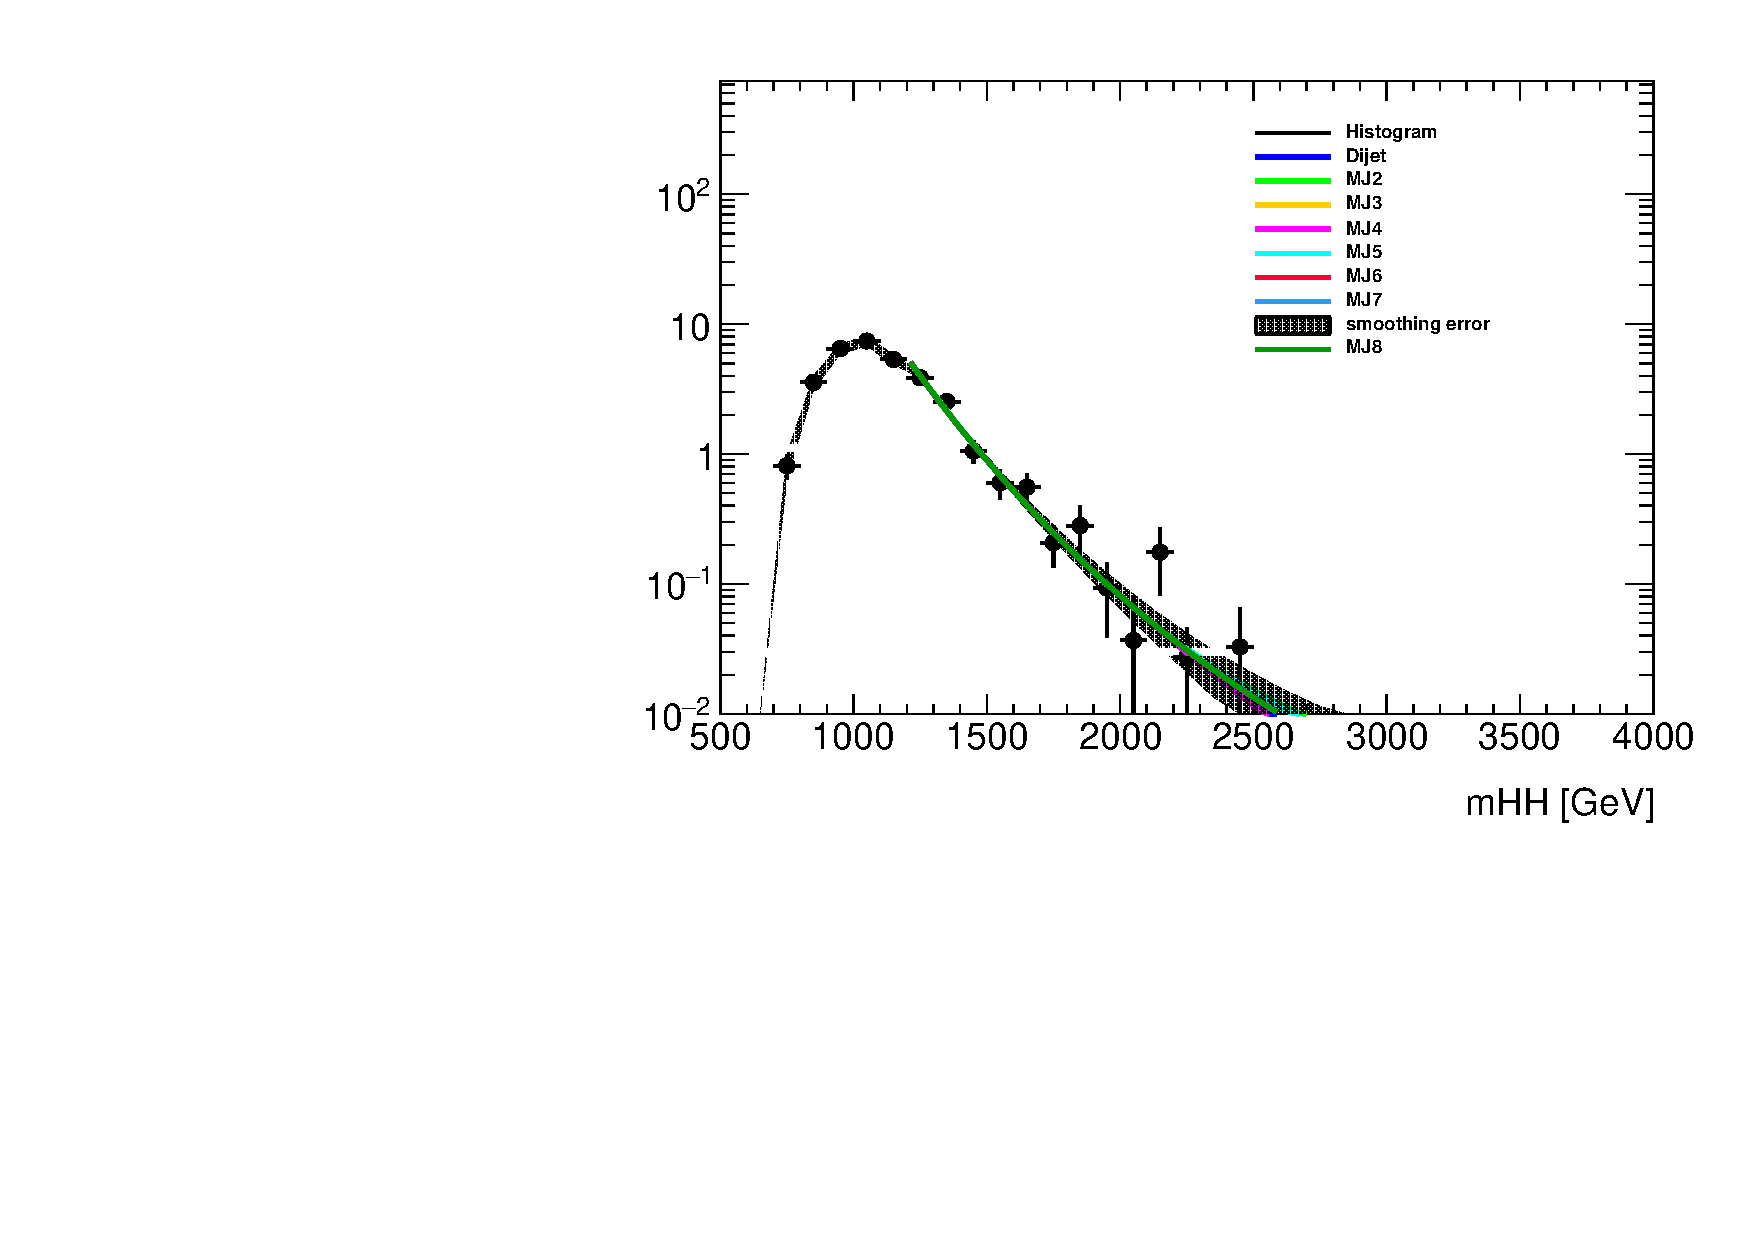
\includegraphics[width=0.48\textwidth,angle=-90]{figures/boosted/Syst_Smooth/smoothFuncCompare_44_comp.pdf}
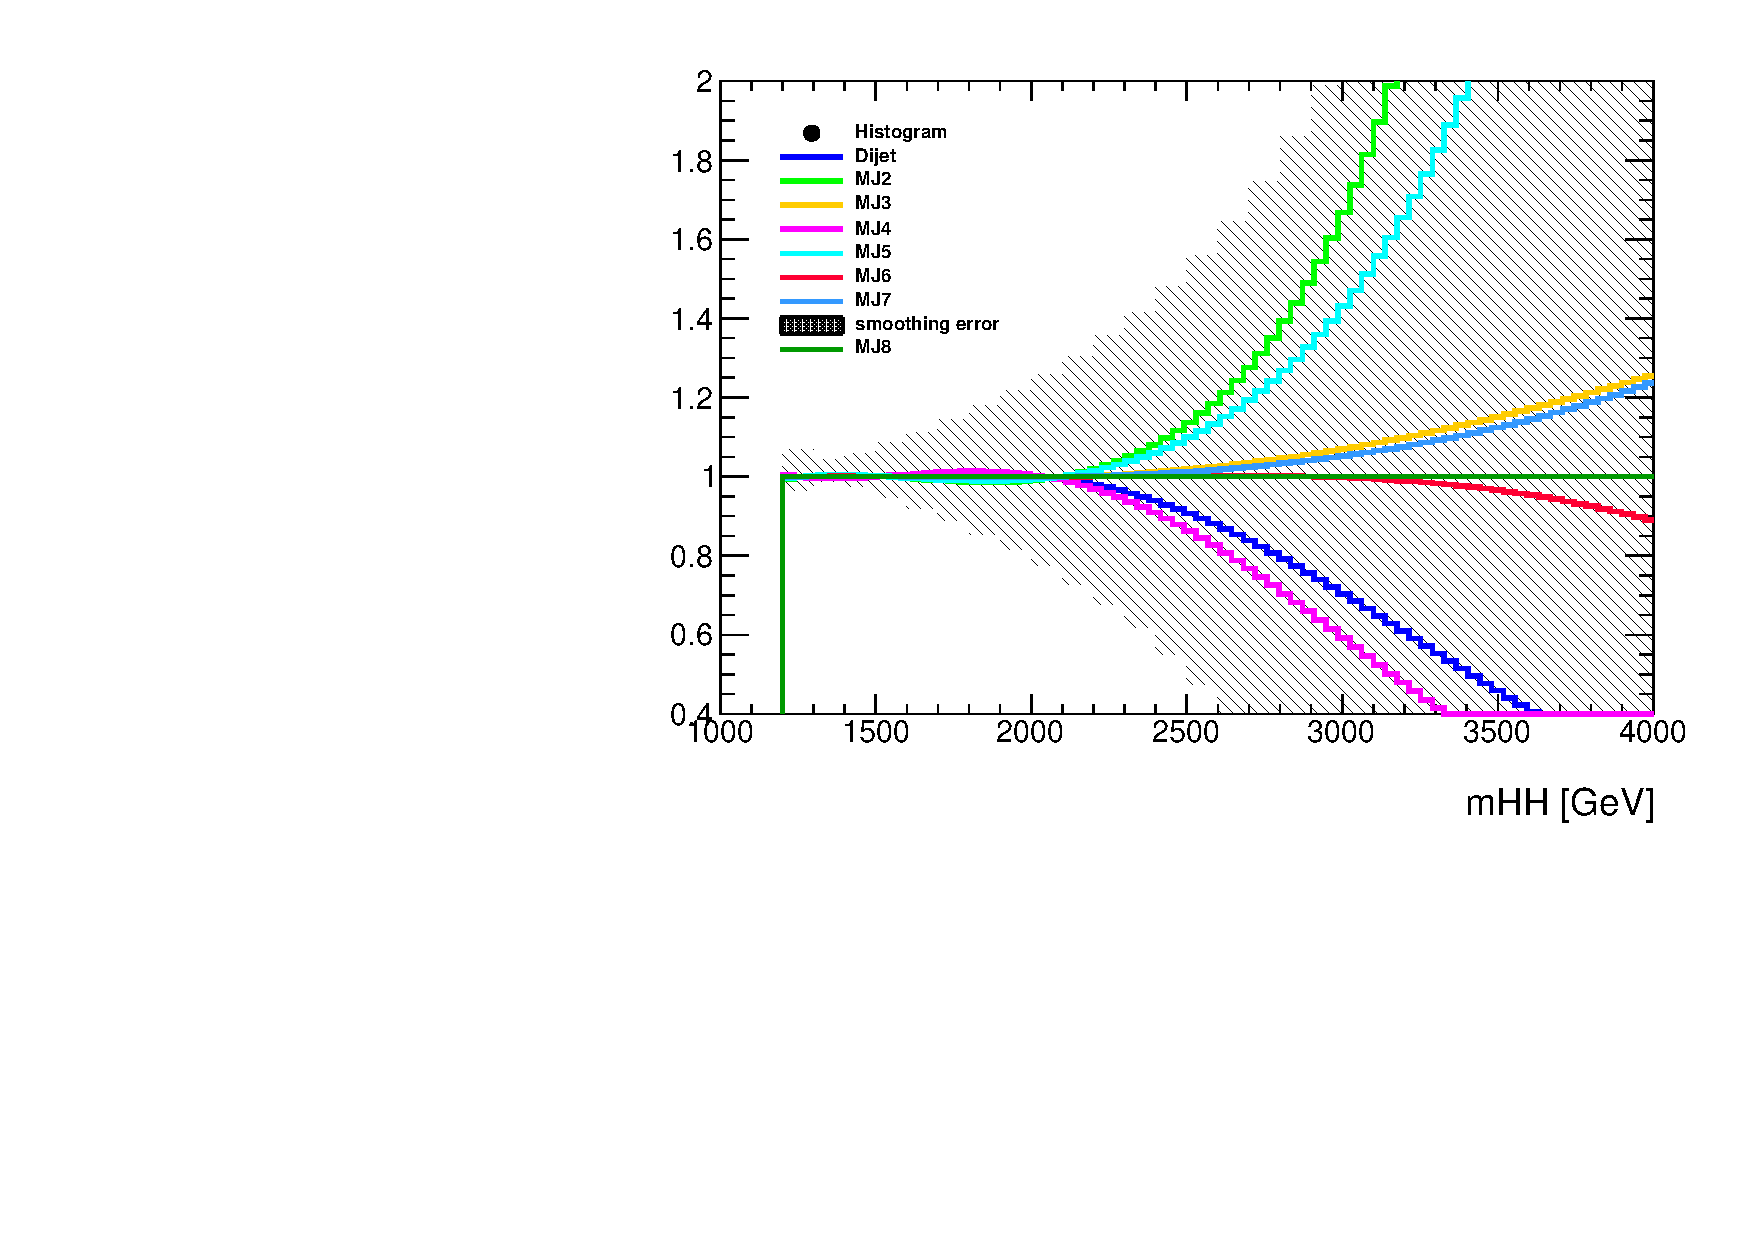
\includegraphics[width=0.48\textwidth,angle=-90]{figures/boosted/Syst_Smooth/smoothFuncCompare_44_comp_ratio.pdf} \\
\caption{ Dijet mass distribution SR prediction fit with several fit functions (left) and the ratio of nominal to fits with different fit functions (right)  for the 2b (top) 3b (middle) and 4b (bottom) samples. The additional fit functions are from Table~\ref{tab:fit_funcs}.}
\label{fig:qcd_fit_funcs_sys}
\end{center}
\end{figure}

%%%
%%%In addition, we examined the consistency between all the variations of the fit parameters from all of the additional function, with the nominal exponential.  The ratio of predictions can be found in Figure~\ref{fig:qcd_fit_funcs_sys_super_ratio}, where the gray lines are the parameter variations from all the additional functions.  Most of these variations are contained in the hashed band, representing the statistical uncertainty of the nominal exponential fit.
%%%
%%%\begin{figure}[htbp!]
%%%\begin{center}
%%%%%\includegraphics[width=0.48\textwidth,angle=-90]{figures/boosted/systematics/QCDFitFunc/QCDFitFuncSys_ratio_super_44.pdf}
%%%% %\includegraphics[width=0.48\textwidth,angle=-90]{figures/boosted/systematics/QCDFitFunc/QCDFitFuncSys_ratio_super_43.pdf}
%%%\caption{The ratio of the nominal exponential QCD prediction of the dijet mass distribution (with hashed band statistical uncertainties) to the predictions of the additional fit functions of Table~\ref{tab:fit_funcs} in the $4b$ (left) and $3b$ (right) signal regions.  \textbf{TO BE UPDATED} }
%%%\label{fig:qcd_fit_funcs_sys_super_ratio}
%%%\end{center}
%%%\end{figure}
%%%
%%%
%%%
%%%As a conservative systematic, the bin-by-bin largest difference between the exponential prediction and the set of additional fit functions or any of the additional function parameter variations is taken as the fit function uncertainty.
%%%
%%%To validate this uncertainty, we perform smoothing on the dijet mass distributions in the CR, and compute the smoothing uncertainties as described above.  The comparison with the CR data can be seen in Figure~\ref{fig:qcd_fit_funcs_sys_check_CR}, where the prediction includes all uncertainties (including the smoothing uncertainty) except the CR shape and normalization uncertainty which was derived from this distribution.  We can see that within uncertainties, the predictions is in good agreement with the CR data.
%%%
%%%\begin{figure}[htbp!]
%%%\begin{center}
%%%%%\includegraphics[width=0.48\textwidth,angle=-90]{figures/boosted/background/DrawCompleteBkgEst_DiJetMass_Pass4GoodTrackJetPass4b77PassCRMass_smoothed.pdf}
%%%% %\includegraphics[width=0.48\textwidth,angle=-90]{figures/boosted/background/DrawCompleteBkgEst_DiJetMass_Pass4GoodTrackJetPass3b77PassCRMass_smoothed.pdf}
%%%\caption{Smoothing prediction applied in the CR compared with data in the $4b$ (left) and $3b$ (right) signal regions. Hashed band show all uncertainties, including the smoothing uncertainties,  except the CR shape and normalization uncertainty which was derived from this distribution.  \textbf{TO BE UPDATED} }
%%%\label{fig:qcd_fit_funcs_sys_check_CR}
%%%\end{center}
%%%\end{figure}
%%%
%%%
%%%
%%%
%%%
%%%The additional smoothing functions are also tested in the case of using the scaled dijet mass distribution, as seen in Figure~\ref{fig:qcd_fit_funcs_sys-scaled}, and the ratio to the nominal fit can be found in Figure~\ref{fig:qcd_fit_funcs_sys_ratio-scaled}, for the $4b$ and $3b$ signal regions.  The same distributions, including also all variations of the parameters of the additional functions within statistical uncertainty, is shown in Figure~\ref{fig:qcd_fit_funcs_sys_super-scaled} and Figure~\ref{fig:qcd_fit_funcs_sys_super_ratio-scaled}.  To be conservative, the maximum bin-by-bin difference between the nominal exponential fit, and any of the variations of the additional functions, is taken as the extrapolation uncertainty.
%%%
%%%
%%%\begin{figure}[htbp!]
%%%\begin{center}
%%%%%\includegraphics[width=0.48\textwidth,angle=-90]{figures/boosted/background/DiJetMassPrime/qcd_smoothfit_FuncComp_44.pdf}
%%%% %\includegraphics[width=0.48\textwidth,angle=-90]{figures/boosted/background/DiJetMassPrime/qcd_smoothfit_FuncComp_43.pdf}
%%%\caption{The QCD prediction of the scaled dijet mass distribution in the $4b$ (left) and $3b$ (right) signal regions, showing the nominal exponential fit (with has band statistical uncertainties) and the additional fits from Table~\ref{tab:fit_funcs}. \textbf{TO BE UPDATED} }
%%%\label{fig:qcd_fit_funcs_sys-scaled}
%%%\end{center}
%%%\end{figure}
%%%
%%%\begin{figure}[htbp!]
%%%\begin{center}
%%%%%\includegraphics[width=0.48\textwidth,angle=-90]{figures/boosted/background/DiJetMassPrime/smoothfunc_ratio_44.pdf}
%%%% %\includegraphics[width=0.48\textwidth,angle=-90]{figures/boosted/background/DiJetMassPrime/smoothfunc_ratio_43.pdf}
%%%\caption{The ratio of the nominal exponential QCD prediction of the scaled dijet mass distribution (with hashed band statistical uncertainties) to the predictions of the additional fit functions of Table~\ref{tab:fit_funcs} in the $4b$ (left) and $3b$ (right) signal regions.  \textbf{TO BE UPDATED} }
%%%\label{fig:qcd_fit_funcs_sys_ratio-scaled}
%%%\end{center}
%%%\end{figure}
%%%
%%%\begin{figure}[htbp!]
%%%\begin{center}
%%%%%\includegraphics[width=0.48\textwidth,angle=-90]{figures/boosted/background/DiJetMassPrime/qcd_smoothfit_FuncCompSuper_44.pdf}
%%%% %\includegraphics[width=0.48\textwidth,angle=-90]{figures/boosted/background/DiJetMassPrime/qcd_smoothfit_FuncCompSuper_43.pdf}
%%%\caption{The QCD prediction of the scaled dijet mass distribution in the $4b$ (left) and $3b$ (right) signal regions, showing the nominal exponential fit (with has band statistical uncertainties) and the additional fits from Table~\ref{tab:fit_funcs}.  \textbf{TO BE UPDATED} }
%%%\label{fig:qcd_fit_funcs_sys_super-scaled}
%%%\end{center}
%%%\end{figure}
%%%
%%%\begin{figure}[htbp!]
%%%\begin{center}
%%%%%\includegraphics[width=0.48\textwidth,angle=-90]{figures/boosted/background/DiJetMassPrime/smoothfunc_ratio_44_extrap.pdf}
%%%% %\includegraphics[width=0.48\textwidth,angle=-90]{figures/boosted/background/DiJetMassPrime/smoothfunc_ratio_43_extrap.pdf}
%%%\caption{The ratio of the nominal exponential QCD prediction of the scaled dijet mass distribution (with hashed band statistical uncertainties) to the predictions of the additional fit functions of Table~\ref{tab:fit_funcs} in the $4b$ (left) and $3b$ (right) signal regions, including all parameter variations of the additional functions.  \textbf{TO BE UPDATED} }
%%%\label{fig:qcd_fit_funcs_sys_super_ratio-scaled}
%%%\end{center}
%%%\end{figure}

\clearpage
%\paragraph{Tests of $\mu_{QCD}$ extrapolation}
%\label{sec:boosted-extrapolation}
%\hspace{0.1mm}\newline
%%\input{Sections/sec-boosted-extrapolations}

